\documentclass[11pt]{article}

\usepackage[square,numbers]{natbib}%for citet

\usepackage{mathptmx,amssymb,amsmath}
\usepackage{fullpage}
\usepackage{enumerate}
\usepackage{fancyvrb}
\usepackage{comment}
\usepackage{listings}
\usepackage{hyperref}
\usepackage[usenames, dvipsnames]{color}
\usepackage{amsthm}
\usepackage{graphicx}
\usepackage{stmaryrd}
\usepackage{mathtools}
\usepackage{float}

\usepackage{ebproof} %for derivation trees
\usepackage{lscape} %to force a page to be in landscape mode
\usepackage{graphicx}
\usepackage{balance}  % for  \balance command ON LAST PAGE  (only there!)
\usepackage{comment}
\usepackage{accents}
\usepackage{lambda,cc}
\usepackage{mathtools} 
\usepackage{array,multirow}
%\usepackage{hhline}
\usepackage{arydshln}
%\usepackage{color}
%\usepackage[usenames, dvipsnames]{xcolor}
\usepackage{xcolor}
%\usepackage{colortbl}
\usepackage{tabularx,booktabs}
\usepackage{mathpartir}
\usepackage{hyperref}
\usepackage[normalem]{ulem}
% commuting diagram packages
\usepackage{tikz}
\usepackage{tikz-cd}
\usetikzlibrary{decorations.pathmorphing}
\usepackage{wrapfig}
%\usepackage{blindtext}% for example text here only
\usepackage{enumitem,kantlipsum} %remove enumerate indent
\usepackage{amssymb}%for arrow labels

\usepackage{listings} % for v-sql example code


%\newcounter{Definition}
%\newcounter{theorem}

\newtheorem{theorem}{Theorem}
\newtheorem{lemma}[theorem]{Lemma}
\newtheorem{proposition}[theorem]{Proposition}
\newtheorem{corollary}[theorem]{Corollary}
\newtheorem{example}[theorem]{Example}
\newtheorem{remark}[theorem]{Remark}
\newtheorem{definition}[theorem]{Definition}


% references
\newcommand{\tabref}[1]{\hyperref[tab:#1]{Table~\ref*{tab:#1}}}
\newcommand{\figref}[1]{\hyperref[fig:#1]{Figure~\ref*{fig:#1}}}
\newcommand{\secref}[1]{\hyperref[sec:#1]{Section~\ref*{sec:#1}}}
\newcommand{\defref}[1]{\hyperref[def:#1]{Definition~\ref*{def:#1}}}
\newcommand{\appref}[1]{\hyperref[app:#1]{Appendix~\ref*{app:#1}}}
\newcommand{\chref}[1]{\hyperref[ch:#1]{Chapter~\ref*{ch:#1}}}
\newcommand{\thmref}[1]{\hyperref[thm:#1]{Theorem~\ref*{thm:#1}}}
\newcommand{\lemref}[1]{\hyperref[lem:#1]{Lemma~\ref*{lem:#1}}}
\newcommand{\exref}[1]{\hyperref[ex:#1]{Example~\ref*{eg:#1}}}

%colors
%\definecolor{deepcarminepink}{rgb}{0.94, 0.19, 0.22}%all shared
%\definecolor{mediumelectricblue}{rgb}{0.01, 0.31, 0.59}%middlename
%\definecolor{frenchblue}{rgb}{0.0, 0.45, 0.73}%lastname
%\definecolor{green(munsell)}{rgb}{0.0, 0.66, 0.47}%iceland
%\definecolor{violet(ryb)}{rgb}{0.53, 0.0, 0.69}%us,invest
%\definecolor{navyblue}{rgb}{0.0, 0.0, 0.5}%v-table
%\definecolor{persimmon}{rgb}{0.93, 0.35, 0.0}%iran
%\definecolor{Plum}{rgb}{0.78, 0.08, 0.52}%us,bank
%\definecolor{ruby}{rgb}{0.88, 0.07, 0.37}%us,bank
%
%\definecolor{light-gray}{gray}{0.95}
%\newcommand{\code}[1]{\colorbox{light-gray}{\texttt{#1}}}

\newcommand{\vamos}{VaMoS'21}
\newcommand{\poly}{Poly'18}
\newcommand{\dbpl}{DBPL'17}
\newcommand{\vldb}{VLDB'21}
\newcommand{\toplas}{TOPLAS'21}

%names
%approaches
\newcommand{\nbf}{NBF}
\newcommand{\ubf}{UBF}
\newcommand{\uav}{UAV}

%shorthands
\newcommand{\ChcExpTxt}{Choice expression}
\newcommand{\DimTxt}{Choice dimension}
\newcommand{\ConfigTxt}{Configuration}
\newcommand{\vdbTxt}{variational database}
\newcommand{\VdbTxt}{Variational database}
\newcommand{\vdbInstTxt}{variational database instance}
\newcommand{\VdbInstTxt}{Variational database instance}
\newcommand{\vqTxt}{variational query}
\newcommand{\VqTxt}{Variational query}
\newcommand{\vqsTxt}{variational queries}
\newcommand{\VqsTxt}{Variational queries}
\newcommand{\vschTxt}{variational schema}
\newcommand{\VschTxt}{Variational schema}
\newcommand{\tenvTxt}{type}
\newcommand{\TenvTxt}{Type}
\newcommand{\vctxTxt}{variation context}
\newcommand{\VctxTxt}{Variation context}
\newcommand{\vRelSchTxt}{variational relation schema}
\newcommand{\VrelSchTxt}{Variational relation schema}
\newcommand{\vrelTxt}{variational relation}
\newcommand{\VrelTxt}{Variational relation}
\newcommand{\presCondTxt}{presence condition}
\newcommand{\PresCondTxt}{Presence condition}
\newcommand{\fexpTxt}{feature expression}
\newcommand{\FexpTxt}{Feature expression}
\newcommand{\vCondTxt}{variational condition}
\newcommand{\VcondTxt}{Variational condition}
\newcommand{\vAttListTxt}{variational attribute list}
\newcommand{\VattListTxt}{Variational attribute list}
\newcommand{\optAttTxt}{optional attribute}
\newcommand{\OptAttTxt}{Optional attribute}
\newcommand{\VlistTxt}{Variational list}
\newcommand{\VsetTxt}{Variational set}
\newcommand{\AnnotVsetTxt}{Annotated variational set}
\newcommand{\AnnotVlistTxt}{Annotated variational list}
\newcommand{\VobjTxt}{Variational object}
\newcommand{\AttTxt}{Attribute}
\newcommand{\RelSchTxt}{Relation schema}
\newcommand{\SchTxt}{Schema}
\newcommand{\RelTxt}{Relation}
\newcommand{\DbInstTxt}{Database instance}
\newcommand{\DbTxt}{Database}
\newcommand{\CondTxt}{Condition}
\newcommand{\vrelAlgTxt}{variational relational algebra}
\newcommand{\VrelAlgTxt}{variational relational algebra}
\newcommand{\typeSys}{type system}
\newcommand{\varPres}{variation preserving}
\newcommand{\VarPres}{Variation preserving}
\newcommand{\FTxt}{Feature}
\newcommand{\QTxt}{Query}
%\newcommand{\VcondTxt}{Variational condition}
\newcommand{\fctTxt}{true feature set}
\newcommand{\osemTxt}{selection semantics /selection /semantics /configuration semantics/ configuring}

%needs names
\newcommand{\nZero}{\textbf{N0}}
\newcommand{\nOne}{\textbf{N1}}
\newcommand{\nTwo}{\textbf{N2}}
\newcommand{\nThree}{\textbf{N3}}
\newcommand{\basic}{\OB{\mathsf{basic}}}
\newcommand{\educational}{\OB{\mathsf{educational}}}

%motivating ex names
\newcommand{\employee}{\OB{\mathit{emp}}}
\newcommand{\eng}{\OB{\mathit{eng}}}
\newcommand{\edu}{\OB{\mathit{edu}}}
\newcommand{\base}{\OB{\mathit{base}}}
\newcommand{\oncamp}{\OB{\mathit{onCamp}}}
\newcommand{\online}{\OB{\mathit{onLine}}}
\newcommand{\vOne}{\OB{V_1}}
\newcommand{\vTwo}{\OB{V_2}}
\newcommand{\vThree}{\OB{V_3}}
\newcommand{\vFour}{\OB{V_4}}
\newcommand{\vFive}{\OB{V_5}}
\newcommand{\tOne}{\OB{T_1}}
\newcommand{\tTwo}{\OB{T_2}}
\newcommand{\tThree}{\OB{T_3}}
\newcommand{\tFour}{\OB{T_4}}
\newcommand{\tFive}{\OB{T_5}}
\newcommand{\fOne}{\OB{f_1}}
\newcommand{\fTwo}{\OB{f_2}}
\newcommand{\engemp}{\OB{\mathit{engineerpersonnel}}}
\newcommand{\othemp}{\OB{\mathit{otherpersonnel}}}
\newcommand{\pers}{\OB{\mathit{personnel}}}
\newcommand{\empacct}{\OB{\mathit{empacct}}}
\newcommand{\empno}{\OB{\mathit{empno}}}
\newcommand{\name}{\OB{\mathit{name}}}
\newcommand{\hiredate}{\OB{\mathit{hiredate}}}
\newcommand{\titleatt}{\OB{\mathit{title}}}
\newcommand{\deptname}{\OB{\mathit{deptname}}}
\newcommand{\salary}{\OB{\mathit{salary}}}
\newcommand{\job}{\OB{\mathit{job}}}
\newcommand{\deptno}{\OB{\mathit{deptno}}}
\newcommand{\dept}{\OB{\mathit{dept}}}
\newcommand{\managerno}{\OB{\mathit{managerno}}}
\newcommand{\empbio}{\OB{\mathit{empbio}}}
\newcommand{\sex}{\OB{\mathit{sex}}}
\newcommand{\birthdate}{\OB{\mathit{birthdate}}}
\newcommand{\fname}{\OB{\mathit{firstname}}}
\newcommand{\lname}{\OB{\mathit{lastname}}}
\newcommand{\course}{\OB{\mathit{course}}}
\newcommand{\ecourse}{\OB{\mathit{ecourse}}}
\newcommand{\student}{\OB{\mathit{student}}}
\newcommand{\teacher}{\OB{\mathit{teacher}}}
\newcommand{\cname}{\OB{\mathit{coursename}}}
\newcommand{\tno}{\OB{\mathit{teacherno}}}
\newcommand{\sno}{\OB{\mathit{studentno}}}
\newcommand{\cno}{\OB{\mathit{courseno}}}
\newcommand{\class}{\OB{\mathit{class}}}
\newcommand{\timeatt}{\OB{\mathit{time}}}
\newcommand{\teach}{\OB{\mathit{teach}}}
\newcommand{\take}{\OB{\mathit{take}}}
\newcommand{\grade}{\OB{\mathit{grade}}}
\newcommand{\isstudent}{\OB{\mathit{std}}}
\newcommand{\isteacher}{\OB{\mathit{instr}}}
\newcommand{\studentnum}{\OB{\mathit{stdnum}}}
\newcommand{\teachernum}{\OB{\mathit{instrnum}}}


% enron email system example names
\newcommand{\enron}{\OB{\mathit{en}}}
\newcommand{\eid}{\OB{\mathit{eid}}}
\newcommand{\emailid}{\OB{\mathit{email\_id}}}
\newcommand{\folder}{\OB{\mathit{folder}}}
\newcommand{\status}{\OB{\mathit{status}}}
\newcommand{\verificationkey}{\OB{\mathit{verification\_key}}}
\newcommand{\publickey}{\OB{\mathit{public\_key}}}
\newcommand{\midatt}{\OB{\mathit{mid}}}
\newcommand{\sender}{\OB{\mathit{sender}}}
\newcommand{\dateatt}{\OB{\mathit{date}}}
\newcommand{\messageid}{\OB{\mathit{message\_id}}}
\newcommand{\subject}{\OB{\mathit{subject}}}
\newcommand{\body}{\OB{\mathit{body}}}
\newcommand{\issigned}{\OB{\mathit{is\_signed}}}
\newcommand{\isencrypted}{\OB{\mathit{is\_encrypted}}}
\newcommand{\isfromremailer}{\OB{\mathit{is\_from\_remaler}}}
\newcommand{\issystemnotification}{\OB{\mathit{is\_system\_notification}}}
\newcommand{\isautoresponse}{\OB{\mathit{is\_autoresponse}}}
\newcommand{\isforwardmsg}{\OB{\mathit{is\_forward\_msg}}}
\newcommand{\rid}{\OB{\mathit{rid}}}
\newcommand{\rtype}{\OB{\mathit{rtype}}}
\newcommand{\rvalue}{\OB{\mathit{rvalue}}}
\newcommand{\rfid}{\OB{\mathit{rfid}}}
\newcommand{\reference}{\OB{\mathit{reference}}}
\newcommand{\forwardaddr}{\OB{\mathit{forwardaddr}}}
\newcommand{\pseudonym}{\OB{\mathit{pseudonym}}}
\newcommand{\suffix}{\OB{\mathit{suffix}}}
\newcommand{\username}{\OB{\mathit{username}}}
\newcommand{\mailhost}{\OB{\mathit{mailhost}}}
\newcommand{\nickname}{\OB{\mathit{nickname}}}
\newcommand{\emailAtt}{\OB{\mathit{email}}}
\newcommand{\employees}{\OB{\mathit{employeelist}}}
\newcommand{\messages}{\OB{\mathit{messages}}}
\newcommand{\recipientinfo}{\OB{\mathit{recipientinfo}}}
\newcommand{\referenceinfo}{\OB{\mathit{referenceinfo}}}
\newcommand{\automsg}{\OB{\mathit{auto\_msg}}}
\newcommand{\forwardmsg}{\OB{\mathit{forward\_msg}}}
\newcommand{\remailmsg}{\OB{\mathit{remail\_msg}}}
\newcommand{\filtermsg}{\OB{\mathit{filter\_msg}}}
\newcommand{\alias}{\OB{\mathit{alias}}}
\newcommand{\id}{\OB{\mathit{id}}}
\newcommand{\scores}{\OB{\mathit{SATscores}}}
%\newcommand{\midatt}{\OB{\mathit{mid}}}
\newcommand{\midCond}{\OB{\midatt = \xvalue}}
\newcommand{\header}{\OB{\mathit{header}}}
\newcommand{\headerAtts}{\OB{\mathit{header\_attributes}}}
\newcommand{\verifiedAt}{\OB{\mathit{verified\_at}}}
\newcommand{\signedBy}{\OB{\mathit{signed\_by}}}
\newcommand{\recievedBy}{\OB{\mathit{recieved\_by}}}
\newcommand{\verStat}{\OB{\mathit{verification\_status}}}
\newcommand{\shouldFilter}{\OB{\mathit{should\_filter}}}

\newcommand{\addressbook}{\OB{\mathit{addressbook}}}
\newcommand{\signature}{\OB{\mathit{signature}}}
\newcommand{\encryption}{\OB{\mathit{encryption}}}
\newcommand{\autoresponder}{\OB{\mathit{autoresponder}}}
\newcommand{\forwardmessages}{\OB{\mathit{forwardmessages}}}
\newcommand{\remailmessage}{\OB{\mathit{remailmessage}}}
\newcommand{\filtermessages}{\OB{\mathit{filtermessages}}}
\newcommand{\basicq}{\OB{\mathit{basic}}}

\newcommand{\addressbookf}{\OB{\mathit{addressbook}}}
\newcommand{\signaturef}{\OB{\mathit{signature}}}
\newcommand{\encryptionf}{\OB{\mathit{encryption}}}
\newcommand{\autoresponderf}{\OB{\mathit{autoresponder}}}
\newcommand{\forwardmsgf}{\OB{\mathit{forwardmessages}}}
\newcommand{\remailmsgf}{\OB{\mathit{remailmessage}}}
\newcommand{\filtermsgf}{\OB{\mathit{filtermessages}}}
\newcommand{\mailhostf}{\OB{\mathit{mailhost}}}

% some specific queries
\newcommand{\Qbasic}{\OB{\nfq_\basicq}}
\newcommand{\Qfilter}{\OB{\nfq_\mathit{filter}}}
\newcommand{\Qforward}{\OB{\nfq_\mathit{forward}}}
\newcommand{\Qencrypt}{\OB{\nfq_\mathit{encrypt}}}
\newcommand{\Qsig}{\OB{\nfq_\mathit{sig}}}
\newcommand{\Qbf}{\OB{\nfq_\mathit{bf}}}
\newcommand{\Qsf}{\OB{\nfq_\mathit{sf}}}
\newcommand{\Qef}{\OB{\nfq_\mathit{ef}}}

\newcommand{\addressbooku}{{ADDRESSBOOK}}
\newcommand{\signatureu}{SIGNATURE}
\newcommand{\encryptionu}{ENCRYPTION}
\newcommand{\autoresponderu}{AUTORESPONDER}
\newcommand{\forwardmsgu}{FORWARDMESSAGES}
\newcommand{\remailmsgu}{REMAILMESSAGE}
\newcommand{\filtermsgu}{FILTERMESSAGES}
\newcommand{\mailhostu}{MAILHOST}

\newcommand{\addressbookl}{{ADDRESSBOOK}}
\newcommand{\signaturel}{SIGNATURE}
\newcommand{\encryptionl}{ENCRYPTION}
\newcommand{\autoresponderl}{AUTORESPONDER}
\newcommand{\forwardmsgl}{FORWARDMESSAGES}
\newcommand{\remailmsgl}{REMAILMESSAGES}
\newcommand{\filtermsgl}{FILTERMESSAGES}
\newcommand{\mailhostl}{MAILHOST}

\newcommand{\faddressbook}{\textcolor{blue} {\OB{\mathit{addressbook}}}}
\newcommand{\fsignature}{\textcolor{blue} {\OB{\mathit{signature}}}}
\newcommand{\fencryption}{\textcolor{blue} {\OB{\mathit{encryption}}}}
\newcommand{\fautoresponder}{\textcolor{blue} {\OB{\mathit{autoresponder}}}}
\newcommand{\fforwardmsg}{\textcolor{blue} {\OB{\mathit{forwardmessages}}}}
\newcommand{\fremailmsg}{\textcolor{blue} {\OB{\mathit{remailmessage}}}}
\newcommand{\ffiltermsg}{\textcolor{blue} {\OB{\mathit{filtermessages}}}}
\newcommand{\fmailhost}{\textcolor{blue} {\OB{\mathit{mailhost}}}}

%\newcommand{\addressbookf}{\OB{\mathit{addressbook}}}
%\newcommand{\signaturef}{\OB{\mathit{signature}}}
%\newcommand{\encryptionf}{\OB{\mathit{encryption}}}
%\newcommand{\autoresponderf}{\OB{\mathit{autoresponder}}}
%\newcommand{\forwardmsgf}{\OB{\mathit{forwardmessages}}}
%\newcommand{\remailmsgf}{\OB{\mathit{remailmessage}}}
%\newcommand{\filtermsgf}{\OB{\mathit{filtermessages}}}
%\newcommand{\mailhostf}{\OB{\mathit{mailhost}}}

\newcommand{\vemployees}{\OB{\mathit{v\_employeelist}}}
\newcommand{\vmessages}{\OB{\mathit{v\_messages}}}
\newcommand{\vrecipientinfo}{\OB{\mathit{v\_recipientinfo}}}
\newcommand{\vreferenceinfo}{\OB{\mathit{v\_referenceinfo}}}
\newcommand{\vautomsg}{\OB{\mathit{v\_auto\_msg}}}
\newcommand{\vforwardmsg}{\OB{\mathit{v\_forward\_msg}}}
\newcommand{\vremailmsg}{\OB{\mathit{v\_remail\_msg}}}
\newcommand{\vfiltermsg}{\OB{\mathit{v\_filtermsg}}}
\newcommand{\vmailhost}{\OB{\mathit{v\_mailhost}}}
\newcommand{\valias}{\OB{\mathit{v\_alias}}}
\newcommand{\midvalue}{\OB{\mathit{X}}}

%query names
\newcommand{\xvalue}{\OB{\mathit{X}}}
\newcommand{\temp}{\OB{\mathit{temp}}}
\newcommand{\tempOne}{\OB{\mathit{temp1}}}
\newcommand{\tempTwo}{\OB{\mathit{temp2}}}
\newcommand{\eq}{\OB{\mathit{empQ}}}
\newcommand{\nfq}{\OB{\mathit{Q}}}
\newcommand{\ntemp}{\OB{\mathit{temp_\mathit{enron}}}}
\newcommand{\deptOne}{\OB{\mathit{``d001"}}}
\newcommand{\mrtable}{\OB{\mathit{mes\_rec}}}
\newcommand{\mretable}{\OB{\mathit{mes\_rec\_emp}}}


% separator
\newcommand{\rSep}{\rn{-}}

%encoding of variational schema in the database
\newcommand{\vdbpc}{\OB{\mathit{vdb\_pcs}\left(\mathit{element\_id}, \mathit{pres\_cond} \right)}}
\newcommand{\tablespc}{\OB{\mathit{tables\_pc}\left(\mathit{table\_name},\mathit{pres\_cond}\right)}}

% table values
\newcommand{\tru}{\OB{\mathit{true}}}
\newcommand{\fls}{\OB{\mathit{false}}}
\newcommand{\NULL}{\OB{\prog{NULL}}}


\newcommand*{\rE}{\rSep\rn{E}}
\newcommand*{\rRefl}{\rn{Refl}}
\newcommand*{\rReflE}{\rRefl\rE}

\newcommand*{\judge}{\rn{Judgement}}
\newcommand*{\empRelRule}{\rn{EmptyRelation}}
\newcommand*{\empRelE}{\empRelRule\rE}
\newcommand*{\relation}{\rn{Relation}}
\newcommand*{\relationE}{\relation\rE}
\newcommand*{\choice}{\rn{Choice}}
\newcommand*{\choiceE}{\choice\rE}
\newcommand*{\product}{\rn{Product}}
\newcommand*{\productE}{\product\rE}
\newcommand*{\setop}{\rn{SetOp}}
\newcommand*{\setopE}{\setop\rE}
%\newcommand*{\diff}{\rn{SetDifference}}
%\newcommand*{\diffE}{\diff\rE}
\newcommand*{\prj}{\rn{Project}}
\newcommand*{\prjE}{\prj\rE}
\newcommand*{\sel}{\rn{Select}}
\newcommand*{\selE}{\sel\rE}
%\newcommand*{\rel}{\rn{RelationRef}}
%\newcommand*{\relE}{\rel\rE}

\newcommand*{\rC}{\rSep\rn{C}}
\newcommand*{\bool}{\rn{Boolean}}
\newcommand*{\boolC}{\bool\rC}
\newcommand*{\nott}{\rn{Neg}}
\newcommand*{\notC}{\nott\rC}
\newcommand*{\conj}{\rn{Conjunction}}
\newcommand*{\conjC}{\conj\rC}
\newcommand*{\disj}{\rn{Disjunction}}
\newcommand*{\disjC}{\disj\rC}
\newcommand*{\attVal}{\rn{AttOptVal}}
\newcommand*{\attValC}{\attVal\rC}
\newcommand*{\attAtt}{\rn{AttOptAtt}}
\newcommand*{\attAttC}{\attAtt\rC}
\newcommand*{\choiceC}{\choice\rC}


%\newcommand*{\rC}{\rSep\rn{C}}
\newcommand*{\rChoice}{\rn{Choice}\rSep}
\newcommand*{\rDist}{\rSep\rn{Dist}}

\newcommand*{\rOpDistC}[1]{\rChoice\rn{#1}\rDist\rC}
\newcommand*{\rSelDistC}{\rOpDistC {Sel}}
\newcommand*{\rPrjDistC}{\rOpDistC {Prj}}
\newcommand*{\rProdDistC}{\rOpDistC {Prod}}

\newcommand*{\rOpDist}[1]{\rChoice\rn{#1}\rDist}
\newcommand*{\rSelDist}{\rOpDist {Sel}}
\newcommand*{\rPrjDist}{\rOpDist {Prj}}
\newcommand*{\rProdDist}{\rOpDist {Prod}}


%intro spl examples
%\newcommand*{\ve}{\OB{\mathit{V}}}
%\newcommand*{\x}{\OB{\mathit{X}}}
%\newcommand*{\y}{\OB{\mathit{Y}}}
%\newcommand*{\msg}{\OB{\mathit{message}}}
%\newcommand*{\sender}{\OB{\mathit{sender}}}
%\newcommand*{\mdate}{\OB{\mathit{date}}}
%\newcommand*{\sbj}{\OB{\mathit{subject}}}
%\newcommand*{\rec}{\OB{\mathit{recepientInfo}}}
%\newcommand*{\rid}{\OB{\mathit{rid}}}
%\newcommand*{\rtype}{\OB{\mathit{rtype}}}
%\newcommand*{\mbody}{\OB{\mathit{body}}}
%\newcommand*{\encrypt}{\OB{\mathit{encrypt}}}
%\newcommand*{\decrypt}{\OB{\mathit{decrypt}}}
%\newcommand*{\encryption}{\OB{\mathit{encryption}}}
%\newcommand*{\decryption}{\OB{\mathit{decryption}}}
%\newcommand*{\employee}{\OB{\mathit{employee}}}
%\newcommand*{\signaturetab}{\OB{\mathit{signature}}}
%\newcommand*{\verification}{\OB{\mathit{verification}}}
%\newcommand*{\sign}{\OB{\mathit{sign}}}
%\newcommand*{\signed}{\OB{\mathit{signed}}}
%\newcommand*{\signKey}{\OB{\mathit{signKey}}}
%\newcommand*{\verify}{\OB{\mathit{verify}}}
%\newcommand*{\isVerified}{\OB{\mathit{isVerified}}}
%\renewcommand*{\mid}{\OB{\mathit{mid}}} %%FYI: you're defining \mid somewhere else, find where!!!!!!!!!!!!!!
%\newcommand*{\isEncrypted}{\OB{\mathit{isEncrypted}}}
%\newcommand*{\encryptionKey}{\OB{\mathit{encryptionKey}}}
%\newcommand*{\ID}{\OB{\mathit{ID}}}
%\newcommand{\faN}{\OB{\mathit{fatherName}}}
%\newcommand{\gender}{\OB{\mathit{gender}}}

%features
\newcommand*{\fName}{\OB{f}}
\newcommand*{\A}{\OB{\fName_1}}
\newcommand*{\B}{\OB{\fName_2}}
\newcommand*{\C}{\OB{\fName_3}}
\newcommand*{\fSet}{\OB{\mathbf{F}}}
\renewcommand*{\dimMeta}{\OB{e}}
\newcommand*{\fModel}{\OB{m}}
\newcommand*{\ffSet}{\OB{\mathbf{E}}}
\newcommand*{\bTag}{\OB{b}}
\newcommand*{\bSet}{\mathbf{B}}
\newcommand*{\config}{\OB{c}}
\newcommand*{\confSet}{\OB{\mathbf{C}}}
\newcommand*{\fct}[1][\config]{\OB{\dimMeta_{#1}^t}}
\newcommand*{\vctx}{\OB{\dimMeta}}

% example feature, feature category and relation names
%\newcommand*{\France}{\OB{\mathit{France}}}
%\newcommand*{\Iceland}{\OB{\mathit{Iceland}}}
%\newcommand*{\US}{\OB{\mathit{US}}}
%\newcommand*{\Iran}{\OB{\mathit{Iran}}}
%\newcommand*{\countryF}{\OB{\mathit{country}}}
%
%\newcommand*{\fType}{\OB{\mathit{type}}}
%\newcommand*{\bank}{\OB{\mathit{bank}}}
%\newcommand*{\stock}{\OB{\mathit{stock}}}
%\newcommand*{\invest}{\OB{\mathit{invest}}}
%
%\newcommand*{\deposit}{\OB{\mathit{deposit}}}
%\newcommand*{\account}{\OB{\mathit{account}}}
%\newcommand*{\amount}{\OB{\mathit{amount}}}
%\newcommand*{\depositor}{\OB{\mathit{depositor}}}
%
%\newcommand*{\member}{\OB{\mathit{member}}}
%\newcommand*{\id}{\OB{\mathit{ID}}}
%\newcommand*{\fN}{\OB{\mathit{firstName}}}
%\newcommand*{\mN}{\OB{\mathit{middleName}}}
%\newcommand*{\lN}{\OB{\mathit{lastName}}}

%spj objects
\newcommand*{\pDB}{\OB{\underline{\db}}}
\newcommand*{\pQ}{\OB{\underline{\q}}}
\newcommand*{\pQSet}{\OB{\underline{\qSet}}}
\newcommand*{\pAtt}{\OB{\underline{\att}}}
\newcommand*{\pAttList}{\OB{\underline{\attList}}}
\newcommand*{\pRel}{\OB{\underline{\rel}}}
\newcommand*{\pRelSch}{\OB{\underline{\relSch}}}
\newcommand*{\pRelCont}{\OB{\underline{\relCont}}}
\newcommand*{\pRelContSet}{\OB{\underline{\relContSet}}}
\newcommand*{\pSch}{\OB{\underline{\sch}}}
\newcommand*{\pInst}{\OB{\underline{\dbInst}}}
\newcommand*{\pInstSet}{\OB{\underline{\dbInstSet}}}
\newcommand*{\pAttSet}{\OB{\underline{\attSet}}}
\newcommand*{\pRelSet}{\OB{\underline{\relSet}}}
\newcommand*{\pRelSchSet}{\OB{\underline{\relSchSet}}}
\newcommand*{\pSchSet}{\OB{\underline{\schSet}}}
\newcommand*{\pAttOpCte}{\OB{\op \pAtt \cte}}
\newcommand*{\pAttOpAtt}{\OB{\op {\pAtt_1}  {\pAtt_2}}}
\newcommand*{\pElem}{\OB{\underline \elem}}
\newcommand*{\pTuple}{\OB{\underline \tuple}}
\newcommand*{\pTab}{\OB{\underline \tab}}

%sql objects
\newcommand*{\sqlQ}{\OB{\underline{sql}}}

%symbols
\newcommand*{\db}{\OB{D}}
\newcommand*{\q}{\OB{q}}
\newcommand*{\att}{\OB{a}}
\newcommand*{\rel}{\OB{r}}
\newcommand*{\tab}{\OB{t}}
\newcommand*{\relSch}{\OB{s}}
\newcommand*{\relCont}{\OB{U}}
\newcommand*{\attList}{\OB{A}}
\newcommand*{\sch}{\OB{S}}
\newcommand*{\dbInst}{\OB{\mathcal{I}}}
\newcommand*{\tuple}{\OB{u}}
\newcommand*{\vTuple}{\tuple}
\newcommand*{\annot}[2][\dimMeta]{\OB{{#2}^{#1}}}
\newcommand*{\elem}{\OB{x}}
\newcommand*{\elemSet}{\OB{X}}
\newcommand*{\cond}{\OB{\theta}}
\newcommand*{\pset}{\OB{\underline {X}}}
\newcommand*{\numRels}{\OB{n}}
\newcommand*{\numTuples}{\OB{k}}
\newcommand*{\numAtts}{\OB{l}}
\newcommand*{\nul}{\OB{\prog{NULL}}}


%set symbols
\newcommand*{\qSet}{\OB{\mathbf{Q}}}
\newcommand*{\dbInstSet}{\OB{\mathbf{I}}}
\newcommand*{\attSet}{\OB{\mathbf{A}}}
%\newcommand*{\tabSet}{\OB{\mathbf{T}}}
\newcommand*{\schSet}{\OB{\mathbf{S}}}
\newcommand*{\relSchSet}{\OB{\mathbf{R}}}
\newcommand*{\relContSet}{\OB{\mathbf{T}}}
\newcommand*{\condSet}{\OB{\boldsymbol{\Theta}}}


% vspj objects
\newcommand*{\vDB}{\db}
\newcommand*{\vSchDef}{\OB{\setDef {{\vRelSch_1 , \ldots, \vRelSch_n}}^\fModel}}
%{\{\widetilde{s}_{R_1}^{F_1}, \ldots, \widetilde{s}_{R_n}^{F_n}\}^\dimMeta}}
\newcommand*{\vdbInst}{\OB{\dbInst}}
\newcommand*{\vdbInstSet}{\OB{\dbInstSet}}
\newcommand*{\vObj}{\OB{o}}
\newcommand*{\vObjSet}{\OB{\mathbf{O}}}
\newcommand*{\vQ}{\OB{\q}}
%\newcommand*{\vRelSch}[1][\pRel]{\OB{{\VVList{s}}_{#1}}}
\newcommand*{\vRelSch}{\OB{\relSch}}
\newcommand*{\vRelCont}{\OB{\relCont}}
\newcommand*{\vSch}{\OB{\sch}}
%\newcommand*{\vSch}{\OB{\VVSet {\mathcal{S}}}}
\newcommand*{\vset}{\OB{X}}
\newcommand*{\vTab}{\tab}
\newcommand*{\vRel}{\rel}
\newcommand*{\vAtt}{\att}

%\makeatletter
%\def\vRel{%
%   \@ifnextchar[%
%     {\vRel@i}
%     {\vRel@i[\dimMeta]}%
%}
%\def\vRel@i[#1]{%
%   \@ifnextchar[%
%     {\vRel@ii{#1}}
%     {\vRel@ii{#1}[\pRel]}%
%}
%\def\vRel@ii#1[#2]{%
%\OB{{#2}^{#1}}
%}
%\makeatother

\newcommand*{\relNum}{\OB{n}}

\makeatletter
\def\vRelConfed{%
   \@ifnextchar[%
     {\vRelConfed@i}
     {\vRelConfed@i[\config]}%
}
\def\vRelConfed@i[#1]{%
   \@ifnextchar[%
     {\vRelConfed@ii{#1}}
     {\vRelConfed@ii{#1}[\pRel]}%
}
\def\vRelConfed@ii#1[#2]{%
\OB{{#2}^{#1}}
}
\makeatother

\makeatletter
\def\optAtt{%
   \@ifnextchar[%
     {\optAtt@i}
     {\optAtt@i[\dimMeta]}%
}
\def\optAtt@i[#1]{%
   \@ifnextchar[%
     {\optAtt@ii{#1}}
     {\optAtt@ii{#1}[\vAtt]}%
}
\def\optAtt@ii#1[#2]{%
%\OB{{\widetilde{#2}}^{#1}}
\OB{\annot[#1]{#2}}
}
\makeatother

%\newcommand*{\vAttt}[2]
%\newcommand*{\attPres}{\OB{F}}
\newcommand*{\vAttList}{\OB{\attList}}
%\widetilde{l}}}
%\newcommand*{\vRelDef}{\OB{\left[\pRel^{\dimMeta}:\vAttList\right]}}

\makeatletter
\def\vRelDef{
   \@ifnextchar[
      {\vRelDef@i}
      {\vRelDef@i[\vRel]}
}
\def\vRelDef@i[#1]{
   \@ifnextchar[
      {\vRelDef@ii{#1}}
      {\vRelDef@ii{#1}[\dimMeta]}
}
\def\vRelDef@ii#1[#2]{
   \@ifnextchar[
      {\vRelDef@iii{#1}{#2}}
      {\vRelDef@iii{#1}{#2}[\vAttList]}
}
\def\vRelDef@iii#1#2[#3]{
\OB{{#1}\left({#3}\right)^{#2}}
}

\newcommand*{\vRelDefNum}[1]{\OB{\vRelDef [\vRel_{#1}] [\dimMeta_{#1}] [\vAttList_{#1}] }}
\newcommand*{\vRelDefNumF}[2]{\OB{\vRelDef [\vRel_{#1}][\vAttList_{#1}][\dimMeta \wedge \dimMeta_{#1}]}}

%\newcommand*{\vRelDef}{\OB{\left[\pRel^{\dimMeta}:\vAttList\right]}}
\newcommand*{\vRelConf}[1][\vRel]{\OB{{#1}^\config}}
\newcommand*{\vAttSet}{\OB{\attSet}}
\newcommand*{\vTabSet}{\OB{\tabSet}}
\newcommand*{\vRelSchSet}{\OB{\relSchSet}}
\newcommand*{\vRelContSet}{\OB{\relContSet}}
\newcommand*{\vSchSet}{\OB{\schSet}}
\newcommand*{\vInstSet}{\OB{\dbInstSet}}
\newcommand*{\empSet}{\OB{\varnothing}}
\newcommand*{\emp}{\OB{\varepsilon}}
\newcommand*{\empAtt}{\OB{\varepsilon}}
\newcommand*{\empRel}{\OB{\varepsilon}}
\newcommand*{\vAttOpCte}{\OB{\op \pAtt \cte}}
\newcommand*{\vAttOpAtt}{\OB{\op {\pAtt_1} {\pAtt_2}}}
\renewcommand*{\tag}[2]{\OB{{#1}^{#2}}}
\newcommand*{\pc}{\OB{pc}}
\newcommand*{\getPC}[1]{\OB{\mathit{pc}{\left({#1}\right)}}}
\newcommand*{\getRel}[1]{\OB{\mathit{rel}{\left({#1}\right)}}}
\newcommand*{\getAtt}[1]{\OB{\mathit{att}{\left({#1}\right)}}}

%conditions
\newcommand*{\pCond}{\OB{\underline{\cond}}}
\newcommand*{\cte}{\OB{k}}
\newcommand*{\pCondSet}{\OB{\underline{\condSet}}}

% variational conditions
\newcommand*{\vCond}{\OB{\cond}}
\newcommand*{\vCondSet}{\OB{\condSet}}

% vspj typing
\newcommand*{\vType}{\OB{\vAttList}}
%\newcommand*{\vContext}{\OB{\vctx}} % --> remove ti

% trans part(Qiaoran)
%\newcommand*{\vSql}{\OB{vq}}
%\newcommand*{\vSqlSet}{\OB{\mathbf{VQ}}}
%\newcommand*{\vRelList}{\OB{rl}}
%\newcommand*{\vRelListSet}{\OB{\mathbf{VrSet}}}
%\newcommand*{\oAttList}{\OB{al}}
%\newcommand*{\oAttListSet}{\OB{\mathbf{Val}}}
%\newcommand*{\vSqlselect}{\textbf{Select} (\vAttList, \vRelList, \vCond)}

% Qiaoran add for translation part
% \newcommand*{\tqS}{\OB{T_Q}}
%\newcommand*{\tqTrans}[1]{\OB{\tqS({#1})}}
%\newcommand*{\trS}{\OB{T_R}}
%\newcommand*{\trTrans}[1]{\OB{\trS({#1})}}

%variational list and set
\newcommand*{\listl}{\OB{l}}
\newcommand*{\sets}{\OB{s}}
\newcommand{\VSet}[1]{\smash{\accentset{\rightarrow}{#1}}}
\newcommand{\VVSet}[1]{\smash{\accentset{\hookrightarrow}{#1}}}
\newcommand{\VList}[1]{\smash{\accentset{\rightarrowtriangle}{#1}}}
\newcommand{\VVList}[1]{\smash{\accentset{\lhook\joinrel\rightarrowtriangle}{#1}}}
\newcommand{\VMap}[1]{\smash{\accentset{\mapsto}{#1}}}


%ops
\newcommand{\Cat}[1]{\mathit{#1}}
\newcommand{\myOR}{\hspace{1.5ex}|\hspace{1.5ex}}
\newcommand{\VVal}[1]{#1'}
\newcommand{\VVVal}[1]{#1''}

\newcommand{\vlift}[1]{\lceil #1 \rceil_S^{S'}}


% defining syntax
\newcommand{\synDef}[2]{\OB{#1 \in #2 }}
\newcommand{\eqq}{\OB{\Coloneqq}}
\renewcommand{\t}{\OB{\prog{true}}}
\newcommand{\f}{\OB{\prog{false}}}

%constraining function
\newcommand{\constrain}[2][\vSch]{\OB{\lfloor #2 \rfloor_{#1}}}

% defining semantics
\newcommand*{\fS}{\OB{\mathbb{E}}}
\newcommand*{\fSem}[2][\config]{\OB{\fS\sem[#1]{#2}}}

\newcommand*{\elemS}{\OB{\mathbb{X}}}
\newcommand*{\elemSem}[2][\config]{\OB{\elemS\sem[#1]{#2}}}

\newcommand*{\elemG}{\OB{\mathcal{G}}}
\newcommand*{\elemGroup}[1][\elem]{\OB{\elemG{\left({#1}\right)}}}

\newcommand*{\qG}{\OB{\mathcal{Q}}}
\newcommand*{\qGroup}[1]{\OB{\qG{\left({#1}\right)}}}

\newcommand*{\cG}{\OB{\mathcal{C}}}
\newcommand*{\cGroup}[1][\vCond]{\OB{\cG{\left({#1}\right)}}}

\newcommand*{\aG}{\OB{\mathcal{A}}}
\newcommand*{\aGroup}[1][\vAttList]{\OB{\aG{\left({#1}\right)}}}

\newcommand*{\oS}{\OB{\mathbb{O}}}
\newcommand*{\oSem}[2][\config]{\OB{\oS\sem[#1]{#2}}}

\newcommand*{\olS}{\OB{\mathbb{A}}}
\newcommand*{\olSem}[2][\config]{\OB{\olS\sem[#1]{#2}}}

\newcommand*{\orS}{\OB{\mathbb{R}}}
\newcommand*{\orSem}[2][\config]{\OB{\orS\sem[#1]{#2}}}

\newcommand*{\otS}{\OB{\mathbb{T}}}
\newcommand*{\otSem}[2][\config]{\OB{\otS\sem[#1]{#2}}}

\newcommand*{\ouS}{\OB{\mathbb{U}}}
\newcommand*{\ouSem}[2][\config]{\OB{\ouS\sem[#1]{#2}}}

\newcommand*{\ovS}{\OB{\mathbb{V}}}
\newcommand*{\ovSem}[2][\config]{\OB{\ovS\sem[#1]{#2}}}

\newcommand*{\osS}{\OB{\mathbb{S}}}
\newcommand*{\osSem}[2][\config]{\OB{\osS\sem[#1]{#2}}}

\newcommand*{\odbS}{\OB{\mathbb{I}}}
\newcommand*{\odbSem}[2][\config]{\OB{\odbS\sem[#1]{#2}}}

%\newcommand*{\eS}{\OB{Q}}
%\newcommand*{\eSem}[2][\config]{\OB{\eS\sem[#1]{#2}}}

\newcommand*{\ecS}{\OB{\mathbb{C}}}
\newcommand*{\ecSem}[2][\config]{\OB{\ecS\sem[#1]{#2}}}

\newcommand*{\eeS}{\OB{\mathbb{Q}}}
\newcommand*{\eeSem}[2][\config]{\OB{\eeS\sem[#1]{#2}}}

%\newcommand*{\tqS}{\OB{T_Q}}
%\newcommand*{\tqSem}[1]{\OB{\tqS\sem[]{#1}}}

% vset operations
\newcommand{\pushIn}[1]{\OB{\downarrow\!\left(#1\right)}}

% spj operations
\newcommand{\pPrj}[2][\pAtt]{\OB{\pi_{#1} #2}}
\newcommand{\pSel}[2][\pCond]{\OB{\sigma_{#1} #2}}
\newcommand{\setDef}[1]{\OB{\{#1\}}}
\newcommand{\pRen}[2][\nameVar]{\OB{\rho_{#1} #2}}

% conditions
\newcommand{\op}[2]{\OB{#1\bullet#2}}
\newcommand{\annd}[1]{\OB{{#1}_1 \wedge {#1}_2}}
\newcommand{\orr}[1]{\OB{{#1}_1 \vee {#1}_2}} 

% vspj operations
\newcommand{\vPrj}[2][\vAttList]{\OB{\pi_{#1} #2}}
\newcommand{\vSel}[2][\vCond]{\OB{\sigma_{#1} #2}}
\newcommand{\vRen}[2][\nameVar]{\OB{\rho_{#1} #2}}
\newcommand{\project}[2]{\OB{\pi_{#1} \left({#2}\right)}}
\newcommand{\projectRel}[2]{\OB{\pi_{#1} {#2}}}
\newcommand{\select}[2]{\OB{\sigma_{#1} \left({#2}\right)}}
\newcommand{\selectRel}[2]{\OB{\sigma_{#1} {#2}}}
\newcommand{\oatt}[2]{\OB{{#1}^{#2}}}
\newcommand{\join}[3]{\OB{\left({#1}\right) \bowtie_{#3} \left({#2}\right)}}
\newcommand{\joinRelL}[3]{\OB{{#1} \bowtie_{#3} \left({#2}\right)}}
\newcommand{\joinRelR}[3]{\OB{\left({#1}\right) \bowtie_{#3} {#2}}}
\newcommand{\joinRel}[3]{\OB{{#1} \bowtie_{#3} {#2}}}
\newcommand{\rename}[2]{\OB{\rho_{#1}  \left({#2}\right)}}
%\newcommand{\choiice}[3]{\OB{\chc [\left({#1}\right)] {\left({#2}\right), \left({#3}\right)}}}
\newcommand{\choiice}[3]{\OB{\chc [\left({#1}\right)] {{#2}, {#3}}}}
%\newcommand{\choiceL}[3]{\OB{\chc [\left({#1}\right)] {{#2}, \left({#3}\right)}}}
%\newcommand{\choiceR}[3]{\OB{\chc [\left({#1}\right)] {\left({#2}\right), {#3}}}}
%\newcommand{\choiceS}[3]{\OB{\chc [{#1}] {\left({#2}\right), \left({#3}\right)}}}
\newcommand{\choiceS}[3]{\OB{\chc [{#1}] {{#2}, {#3}}}}
%\newcommand{\choiceSL}[3]{\OB{\chc [{#1}] {{#2}, \left({#3}\right)}}}
%\newcommand{\choiceSR}[3]{\OB{\chc [{#1}] {\left({#2}\right), {#3}}}}
%\newcommand{\chc}[2][\dimMeta]{\OB{#1\chcL#2\chcR}}

% query type environment
%\newcommand{\env}[4][\vctx][\vSch]{\OB{#1,#2 \vdash#3:#4}}
\makeatletter
\def\env{
  \@ifnextchar[
    {\env@i}
    {\env@i[\vctx]}
}
\def\env@i[#1]{
  \@ifnextchar[
    {\env@ii{#1}}
    {\env@ii{#1}[\vSch]}
}
\def\env@ii#1[#2]#3#4{
{\OB{#1,#2 \vdash#3:#4}}
}
\makeatother

\newcommand{\envWithoutVctx}[3][\vSch]{\OB{#1 \vdash #2 : #3}}
\newcommand{\explEnv}[3][\vSch]{\OB{#1 \vDash #2 : #3}}
\newcommand{\pEnv}[3][\pSch]{\OB{#1 \vdash #2 : #3}}
\newcommand{\envWithSchema}[2][\OB{\vctx}]{\env[#1]{\vRel}{#2}}
\newcommand{\envRelInSch}[2][\vSch]{\env[#1]{#2}{\vType}}
\newcommand{\envOne}[1][\vctx]{\env[#1]{\vQ_1}{\envInContext [\vctx_1] \vType_1}}
\newcommand{\envTwo}[1][\vctx]{\env[#1]{\vQ_2}{\envInContext [\vctx_2] \vType_2}}
\newcommand{\envPrime}{\env{\vQ}{\envInContext[\VVal \vctx]{\VVal \vType}}}

% condition type environment
\newcommand{\envCond}[2][\vctx, \vType]{\OB{#1\vdash #2}}
\newcommand{\envCondAnnot}[2][\vctx, {\pushIn{\annot [\VVal \vctx] \vType}}]{\OB{#1\vdash #2}}

% type and variation context
\newcommand{\envL}{\OB{\lfloor}}
\newcommand{\envR}{\OB{\rfloor}}
\newcommand{\envInContext}[2][\vctx]{\OB{{#2}^{#1}}}
\newcommand{\envEval}[2]{#1 \equiv #2}
\newcommand{\imply}{\OB{\rightarrow}}
\newcommand{\subsume}[2]{\OB{#1 \prec #2}}
\newcommand{\subsumeExpl}[2]{\OB{#1 \preccurlyeq #2}} 
\newcommand{\nsubsume}[2]{\OB{#1 \not \prec #2}}

% object in a variational context
\newcommand{\relInContext}[2][\vRel]{\OB{#1^{#2}}}
\newcommand{\attInContext}[2][\vAtt]{\OB{#1^{#2}}}
\newcommand{\defType}[2][\vType]{\OB{#2: #1}}


% satisfiability function
\newcommand{\sat}[1]{\OB{\mathit{sat}{\left(#1\right)}}}
\newcommand{\unsat}[1]{\OB{\mathit{unsat}{\left(#1\right)}}}
\newcommand{\taut}[1]{\OB{\mathit{taut}{\left(#1\right)}}}

% dbms
\renewcommand{\dom}[2][\vdbInst]{\OB{\mathit{dom}_{#1}{\left(#2\right)}}}
\newcommand{\type}[1][\pAtt]{\OB{\mathit{type}{\left({#1}\right)}}}
\newcommand{\attr}[1][\pRel]{\OB{\mathit{attr}{\left(#1\right)}}}
\newcommand{\arity}[1][\pRel]{\OB{\mathit{arity}{\left(#1\right)}}}
\newcommand{\feat}[2][\vObj]{\OB{\mathit{presCond_{#1}}\left(#2\right)}}
\newcommand{\obj}[1]{\OB{\mathit{obj}\left(#1\right)}}

%\newcommand{\chc}[2][\dimMeta]{\OB{#1\chcL#2\chcR}}
%\newcommand{\chcPP}[3][\dimMeta]{\chc[#1]{\prog{#2},\prog{#3}}}
%\newcommand{\chcPPP}[4][\dimMeta]{\chc[#1]{\prog{#2},\prog{#3},\prog{#4}}}

% special equalities
\newcommand{\spcEq}[1][0cm]{\OB{\hspace{#1}=}}
\newcommand{\spcEquiv}[1][0cm]{\OB{\hspace{#1}\equiv}}


% operations w.r.t. c
\newcommand{\equivc}{\OB{\equiv_{\config}}}


% enumeration and indexing 
\newcommand{\vvn}[2]{\OB{{#1_1}^{#2_1}, \ldots, {#1_n}^{#2_n}}}

% formulation in general
\newcommand{\paran}[1]{\OB{\left(#1\right)}}



%%%
%%% Formatting details
%%%
\sloppy
\sloppypar
\widowpenalty=0
\clubpenalty=0
\displaywidowpenalty=0
\raggedbottom
\pagestyle{plain}


% \topskip0pt
% \parskip0pt
% \partopsep0pt


\def\denseitems{
    \itemsep1pt plus1pt minus1pt
    \parsep0pt plus0pt
    \parskip0pt\topsep0pt}



\begin{document}

%\title{Variational Database Management System: Theory and Application}
%\title{Variational Database: Theory, Tool, and Application}
\title{Theory and Implementation of a Variational Database Management System}

\author{Parisa S. Ataei\\
Thesis Proposal \\
Submitted November 3rd, 2020
}
\date{}

\maketitle

\section*{Abstract}
Many problems require working with data that varies in its structure and content. Likewise, many tools and techniques have been developed for dealing with variation in databases with respect to time (e.g., work on database evolution) or space (e.g., work on data integration).
%various instances of this problem, for example, work on database evolution addresses the need to deal with variation in data over time, and work on data integration addresses the need to work with variation in data from different sources. 
%Many problems require working with data that varies in its structure and content. Likewise, many tools and techniques have been developed for dealing with various instances of this problem, for example, work on database evolution addresses the need to deal with variation in data over time, and work on data integration addresses the need to work with variation in data from different sources. 
However, these specialized approaches neither cover all data variation needs nor provide a solution to deal with database variation both in time and space simultaneously.
%[, such as the need to work with different variants of a database corresponding to different configurations of a software system, or data that varies both over time and by source]. 
%In this paper, we define a generic framework that considers variation orthogonal to database. It captures variation in the structure and content of a database and allows queries to express variation in information need.
%In this paper, we introduce an extension of relational database theory that incorporates variation as an orthogonal concern that allows expressing variation in information need.
%We define variational schemas for describing variation in the structure of a database
%variational queries for expressing variation in information needs, 
%and variational databases for capturing variation in content. 
%We define a type system relating variational queries with variational schemas, and 
%
%Variation occurs in databases in many different forms and contexts. For
%example, a single database schema evolves over time, data from different
%sources may be combined, and the various configurations of a software product
%line (SPL) may have different data needs.
%
%This variability exists in two dimensions: ``time'' (for example, a database
%evolves over time and consequently its schema changes) and ``space'' (for
%example, clients of a Software Product Line (SPL) require different variants
%of the database used by the software).
%
%While approaches have been developed to deal with many such scenarios,
%particularly in the fields of database evolution and data integration, there is
%no general solution that treats variation as a general and orthogonal concern
%in databases. This is a problem when various kinds of variation intersect,
%such as during the evolution of a SPL.
%
In this research, we propose a generic framework that considers
\emph{variation} orthogonal to relational databases. 
We extend the relational database theory to incorporate variation
explicitly in databases and the query language:
we define \emph{variational schemas} for describing variation in the structure of a database
\emph{variational queries} for expressing variation in information needs, 
and \emph{variational databases} for capturing variation in content. 
%We define a type system relating variational queries with variational schemas
%
Although the model underlying variational database is simple, encoding variation
explicitly in databases introduces complexity akin to using preprocessing
directives in software. 
%The question then arises: is this a good idea?
We evaluate the feasibility of this approach by systematically developing two case studies
that illustrate how different kinds of variation needs can be encoded and
integrated in a variational database and how the
corresponding information needs can be expressed as variational queries.
%
We also design and implement a variational database management system as an abstraction layer over a traditional relational database. We demonstrate the applicability and feasibility of our approach on our two case-studies.


\section{Introduction}
\label{sec:intro}


\begin{comment}
simple streamline direction:
- variation in db is everywhere
- active research for some instances of it
- other instances aren't well-covered and well-supported
- the combination of instances

a general solution that 
- can model variation for well-covered variation
- others
\end{comment}

%\structure{openning}
%Variation in databases appears abundantly in different forms and contexts.

Variation in databases arises when multiple database instances 
conceptually represent the same database, but, differ
slightly either in their schema and/or content. 
%
Managing variation in databases is a perennial problem in database literature
and appears in different forms and contexts.
Specific cases of this problem has been extensively studied including 
schema evolution~\cite{}, 
data integration~\cite{}, 
and database versioning~\cite{},
where each instance has a context-specific solution that is hard-wired
to the constrained problem definition. 
%
While schema
evolution approaches deal with variation in the schema (i.e., the structure
of the data) database versioning and data integration systems 
manage variation in the content of the database. Yet, the database
community does not consider them as instances of the same problem.
%For example, 
%approaches designed to manage schema evolution over time force
%database administrators to add timestamps to each version of the schema
%in the format that is used by the approach~\cite{} while systems designed
%to manage database versioning force database administrators to use 
%version numbers .

Consider schema evolution which is an instance of schematic variation in databases
that is well-supported~\cite{SchEvolRA90McKenzie, 
schVersioning97Castro, tempSchEvol91Ariav, tsql95Snodgrass, 
prima08Moon}.
Changes applied to the schema over time are \emph{variation} 
in the database and every time the database evolves, a new
\emph{variant} is generated.
%which needs to coexists in parallel
%with other variants.
Current solutions addressing schema
evolution rely on temporal nature of schema evolution by using
timestamps~\cite{SchEvolRA90McKenzie, schVersioning97Castro, 
tempSchEvol91Ariav, tsql95Snodgrass} 
or keeping an external file of time-line history of 
changes applied to the database~\cite{prima08Moon}. 
These approaches only consider variation in time and do not
%However, none of them 
incorporate the time-based changes into
the database directly, rather they \emph{simulate} the effect of these changes,
resulting in brittle systems.

Database-backed software produced by software product line (SPL) 
is an example where variation arises in databases and is poorly 
supported. SPL is an
approach to developing and maintaining software-intensive systems 
in a cost-effective, easy to maintain manner by accommodating variation
in the software that is being reused. 
%The products of a SPL pertain to a
%common application domain or business goal. 
%They also have a common
%managed set of features that describe the specific need for a product. 
%They share 
%a common codebase which is used to produce a product with respect to its set of 
%selected (enabled) features
In SPL, a common codebase is shared and used to produce products w.r.t.
a set of selected (enabled) features~\cite{splBook}. 
% from the SPL feature set designed to describe
%specific needs for products~\cite{splBook}. 
Different products of a SPL typically have different
sets of enabled features or are tailored to run in different environments. These
differences impose different data requirements which creates variation in space 
in the shared database used in the common codebase. 
%Hence, 
%each product has its own database variant.
%For example, different legal
%requirements often require tracking different data in products tailored for use
%in different countries or regions~\cite{splBook}.
%Different data requirements results in different desired data which 
%creates database variants. 
%
%
%The database variants corresponding to software products differ mainly 
%in their schema, a relation/attribute can either be included or excluded for a 
%specific software product~\cite{vdbSpl18ATW}.
The variation is in the form of exclusion/inclusion of tables/attributes based on
selected features for a product~\cite{vdbSpl18ATW}.
%
In practice, software systems produced by a SPL are accommodated with a database that
has all attributes and tables available for all variants-- a database with universal schema~\cite{vdbSpl18ATW}. 
Unfortunately, this approach is
inefficient, error-prone, and filled with lots of null values since not all attributes and tables
are valid for all variant products. A possible solution to this could be defining views on 
the universal database per software variant and write queries for each variant against its 
view~\cite{vdbSpl18ATW}.
However, this is burdensome, expensive, and costly to maintain since it 
requires developers to generate and maintain numerous view definitions
in addition to manually generating
and managing the mappings between views and the universal schema for each product.


Additionally, the software product line (SPL) community has realized that 
variation in software development travels to its artifact including the database.
%
SPL is an
approach to developing and maintaining software-intensive systems 
in a cost-effective, easy to maintain manner by accommodating variation
in the software that is being reused. 
%
In SPL, a common codebase is shared and used to produce products w.r.t.
a set of selected (enabled) features~\cite{splBook}. 
%
Different client's products of a SPL typically have different
sets of enabled features or are tailored to run in different environments. These
differences impose different data requirements which creates variation in space 
in the shared database used in the common codebase. 
%
The SPL community has closed
the gap of variation appearing in database schema while developing software
and the database schema used in client's application by
encoding variation explicitly in data model, called \emph{variable data model}~\cite{}. 
However, the direct encoding of variation has not been extended to the
database itself by these approaches. 

To the best of our knowledge, 
there is no generic solution that manages all possible kinds of
variation in databases. Thus, we explore the idea of considering
variation as a \emph{first-class citizen} in databases. Such exploration
poses questions such as: How can variation be represented in a generic
expressive manner? How can variation be encoded explicitly in databases?
What are the benefits and drawbacks of explicitly encoding variation in 
databases? How applicable and feasible it is to encode variation 
directly in databases?

To answer these research questions we propose the following research goals:

\begin{itemize}
\item Objective 1: Identify the kinds of variation existing in relational databases in 
different application domains.
\item Objective 2: Design a query language and implement a database management 
system that accommodate  variations identified in objective 1.
\item Objective 3: Demonstrate how the proposed system can be used to manage
variation in databases in different application domains.
\item Objective 4: Mechanize proofs of properties of the language and the system.
% maybe as a stretch goal
%\item Objective 5: Generalize the encoding of variation and the design of the query 
%language to cover more kinds of variation.
\end{itemize}


%----------------------------------------------------------------------------

%are instances of the general problem that are
%not well-studied, resulting in using manual approaches that burden experts.
%Moreover, different kinds of variation can interact which cannot be addressed
%by current approaches due to lack of a general solution to managing 
%different kinds of variation in databases.
%%In this paper, 
%To understand 
%we provide a fundamental solution to managing
%variation in databases by considering variation explicitly as 
%a \emph{first-class citizen}
%in the system, allowing for encoding different kinds of variation.
%
%
%%\structure{the following paragraphs are funnel}
%%\point{Schematic and content-level variation in DBs that conceptually 
%%represent the same data.}
%Variation in databases arises when multiple database instances 
%conceptually represent the same database, but, differ
%slightly either in their schema and/or content. 
%%These database
%%instances coexist in parallel.
%The variation in schema and/or content occurs in two dimensions:
%time and space. Variation in space refers to different variants of database that
%coexist in parallel while variation in time refers to the evolution of 
%database, similar to variation observed in software~\cite{EricSPLEvolve19}. 
%Note that variation in a database can occur due to both dimensions
%at the same time.
%
%
%%\point{Schema evolution is an instance of variation in databases
%%that is well-supported.}
%%Explains how schema evolution (which is unavoidable) 
%%is an instance of variation in databases.
%%And mentions some of the current solutions, emphasizing that
%%they cannot address other instances of the problem.
%Schema evolution is an instance of schematic variation in databases
%that is well-supported~\cite{SchEvolRA90McKenzie, 
%schVersioning97Castro, tempSchEvol91Ariav, tsql95Snodgrass, 
%prima08Moon}.
%Changes applied to the schema over time are \emph{variation} 
%in the database and every time the database evolves, a new
%\emph{variant} is generated.
%%which needs to coexists in parallel
%%with other variants.
%Current solutions addressing schema
%evolution rely on temporal nature of schema evolution by using
%timestamps~\cite{SchEvolRA90McKenzie, schVersioning97Castro, 
%tempSchEvol91Ariav, tsql95Snodgrass} 
%or keeping an external file of time-line history of 
%changes applied to the database~\cite{prima08Moon}. 
%These approaches only consider variation in time and do not
%%However, none of them 
%incorporate the time-based changes into
%the database directly, rather they \emph{simulate} the effect of these changes,
%resulting in brittle systems.
%
%
%%\point{Database-backed software produced by SPL is an instance
%%of variation in databases that is poorly managed in practice.}
%%Explains SPL briefly and how variation appears in databases used to
%%store data for software produced by SPL. As well as how poorly it is 
%%managed in practice.
%Database-backed software produced by software product line (SPL) 
%is an example where variation arises in databases and is poorly 
%supported. SPL is an
%approach to developing and maintaining software-intensive systems 
%in a cost-effective, easy to maintain manner by accommodating variation
%in the software that is being reused. 
%%The products of a SPL pertain to a
%%common application domain or business goal. 
%%They also have a common
%%managed set of features that describe the specific need for a product. 
%%They share 
%%a common codebase which is used to produce a product with respect to its set of 
%%selected (enabled) features
%In SPL, a common codebase is shared and used to produce products w.r.t.
%a set of selected (enabled) features~\cite{splBook}. 
%% from the SPL feature set designed to describe
%%specific needs for products~\cite{splBook}. 
%Different products of a SPL typically have different
%sets of enabled features or are tailored to run in different environments. These
%differences impose different data requirements which creates variation in space 
%in the shared database used in the common codebase. 
%%Hence, 
%%each product has its own database variant.
%%For example, different legal
%%requirements often require tracking different data in products tailored for use
%%in different countries or regions~\cite{splBook}.
%%Different data requirements results in different desired data which 
%%creates database variants. 
%%
%%
%%The database variants corresponding to software products differ mainly 
%%in their schema, a relation/attribute can either be included or excluded for a 
%%specific software product~\cite{vdbSpl18ATW}.
%The variation is in the form of exclusion/inclusion of tables/attributes based on
%selected features for a product~\cite{vdbSpl18ATW}.
%%
%In practice, software systems produced by a SPL are accommodated with a database that
%has all attributes and tables available for all variants-- a database with universal schema~\cite{vdbSpl18ATW}. 
%Unfortunately, this approach is
%inefficient, error-prone, and filled with lots of null values since not all attributes and tables
%are valid for all variant products. A possible solution to this could be defining views on 
%the universal database per software variant and write queries for each variant against its 
%view~\cite{vdbSpl18ATW}.
%However, this is burdensome, expensive, and costly to maintain since it 
%requires developers to generate and maintain numerous view definitions
%in addition to manually generating
%and managing the mappings between views and the universal schema for each product.
%
%
%%\point{Schema evolution meets SPL evolution and results in databases
%%used in SPL that their schemas evolve over time.}EricSPLEvolve19, splEvolveBP14
%%Mentions that SPL evolution is hot topic. Part of this evolution is database
%%evolution. This is where two instances of managing variation in databases
%%interact and even the well-supported systems for schema evolution cannot
%%address it. 
%Software evolution is unavoidable, so is its artifacts evolution, 
%including databases~\cite{dbSPLevolve}.
%%Variation in software development is unavoidable and 
%This is where two instances of managing 
%variation in databases (schema evolution and database-backed software 
%developed by SPL) interact.
%% and variation occurs both in time and space. 
%While there are solutions to schema evolution
%they cannot adapt to a new situation because they only provide a solution to
%variation of databases in time and cannot encode the interaction of database variation in
%time and space.
%%dismiss variation of databases in space, 
%%i.e., they dismiss that database variants that have been created due to variation
%%in time must coexist in parallel (a property of variation in 
%%space~\cite{EricSPLEvolve19}). 
%We motivate this case through an example in \secref{mot}.
%%We use this case as our motivating example in \secref{mot} and explain it 
%%in more details.
%
%%\structure{knowledge gap + challenge}
%%\point{Reiterate the knowledge gap. Introduce the challenge.} 
%%Reiterates the knowledge gap. Explains the challenge:
%%The challenge then becomes encoding variation in databases
%%that can model different instances and satisfy different specialists' needs 
%%at different stages (like development, deployment, information extraction, etc).
%%%Explains the challenge as incorporating variation in databases s.t. all 
%%%database variants are gathered in one place. 
%%Also, itemizes the users' 
%%needs in such an environment: 
%%1) Query some/all variants simultaneously and selectively.
%%2) Track the original variant of a piece of data and the variation applied
%%to it through a query.
%%3) Deploy the database and its queries to a variant of it.
%As we have shown, 
%variation in databases w.r.t. time and space is abundant and inexorable~\cite{dbDecay16Stonebraker};
%impacts DBAs, data scientists, and developers significantly~\cite{dbSPLevolve}; 
%and appears in different contexts. Various research has studied variation of databases
%in time and space, however, they all consider only one of these dimensions and
%are extremely tailored to a specific context. This becomes a problem when 
%the two dimensions and different contexts interact. Hence, the challenge becomes
%%offering a fundamental generic framework that 
%incorporating variation in databases s.t. it can model different instances of variation
%in different contexts and it satisfies different specialists' needs at different stages,
%e.g., development, information extraction, and deployment. 
%%
%%We categorize these needs and explain them throughout the paper:
%%\begin{enumerate}[leftmargin=*]
%%\item [\textbf{N0}]Have access to all database variants at a given time
%%\item [\textbf{N1}]Query multiple database variants simultaneously and selectively
%%\item [\textbf{N2}]Keep track of which variants a piece of data belongs to and ensuring that 
%%         it is maintained throughout a query
%%\item [\textbf{N3}]Deploy one variant of the database and its associated queries.
%%\end{enumerate}
%%\structure{proposed solution}
%%%\point{challenge: capturing/representing variability in the database + 
%%%(put-all-together origin-tracking framework) + solution (contributions).}
%%%\structure{point-last.}
%%Therefore, 
%%\emph{
%%how can we incorporate variability in databases to allow for
%%expressive queries over multiple
%%database variants selectively and simultaneously while keeping
%%track of the original variation of data and variation applied to it by
%%a query
%%%without violating data provenance
%%%and 
%%s.t. it is applicable in different contexts?}
%Our contributions in this paper address this challenge:
%\begin{itemize}[leftmargin=*]
%\itemsep0em
%%[wide, labelwidth=!, labelindent=0pt, topsep=1pt]
%%[leftmargin=*]
%\item We provide a framework to capture variation within a database using
%propositional formulas over  
%sets of features, called \emph{feature expressions}, following~\cite{vdb17ATW}.
%\item We incorporate feature expressions  into both the structure (schema) and
%content (tuples) of the database, introducing \emph{variational schemas}, \secref{vsch}, 
%and \emph{variational tables}, \secref{vtab}, and together \emph{VDBs},
%\secref{vdb}.
%%, satisfying \textbf{N0} and first part of \textbf{N2}.
%\item To express user information needs we define the 
%\emph{variational relational algebra} query language,
%%which is 
%a combination of relational algebra and 
%choice calculus~\cite{EW11tosem,Walk13thesis}, \secref{vrel-alg}.
%%, 
%%satisfying \textbf{N1}.
%Users query a VDB by a \emph{variational query}, \secref{vq}.
%\item 
%To make variational queries more useable and easier to understand, respectively,
%we define 
%a static type system, \secref{type-sys},
%and \emph{variation-minimiztion} rules, \secref{var-min}.
%%to make it easier to understand and more useable. 
%%rules to minimize 
%%variation in v-query, \secref{var-min}, to provide better
%%efficiency and usability. 
%%This completes satisfiability of \textbf{N2}.
%\item To query a 
%variational database and receive clear results
%we implement \emph{Variational Database Management System (VDBMS)}, \secref{impl}.
%%,
%%satisfying all four needs: \textbf{N0}-\textbf{N3}.
%%\textbf{N1}, \textbf{N2}, and \textbf{N3}.
%\end{itemize}
%
%%\point{evaluate VDBMS + its pay off}
%%To evaluate VDBMS, 
%VDBMS provides new functionality to databases by accounting for 
%schematic and content-level variation. We provide two use cases of how VDBMS can
%model the schema evolution and SPL instances of variation in databases
%for two real-world databases,
%%(employee database\footnote{\url{https://github.com/datacharmer/test_db}} 
%%and Enron email data corpus\footnote{\url{http://www.ahschulz.de/enron-email-data/}}),
%\secref{exp-disc}. 
%%We also adopt practical queries from~\cite{prima08Moon} and~\cite{emailSPL},
%%respectively,
%%for our use cases to assess VDBMS, \secref{exp-qs}.
%We hypothesize that it especially pays
%off when there is lots of variation in the database and the user needs to query
%many of the variants simultaneously, \secref{exp-disc}. 
%%To examine our hypothesis,  
%%we adopt two real-world databases 
%%from two different contexts (schema evolution and SPL) and
%%generate their counterpart VDBs (based on the changes applied to them).
%%, assess
%%the performance of VDBMS using a set of queries within each context, and
%%finally analyze and discuss the results, \secref{exp-disc}.
%%Our experiments show ...
%%, elucidated more in \secref{exp-disc}.
%
%
%
%%%\begin{comment}
%%%vamos intro:
%%\section{Introduction}
%%\label{sec:intro}
%%
%%%\NOTE{High-level comment: avoid abbreviations like ``w.r.t.'' (I usually edit
%%%most of these out when revising your writing), or at least use them very
%%%sparingly. ``i.e.'' and ``e.g.'' are OK in parentheticals (e.g.\ this is fine),
%%%but should be avoided in the flow of text, e.g.\ this is awkward.}
%%
%%%\NOTE{Maybe first paragraph on how variation in software leads to variation in
%%%databases and vice-versa? Then get into how this breaks down into time and
%%%space.}
%%
%%%\TODO{we show feasibility of our approach. feasibility study.}
%%%
%%%\TODO{var in softwar. var in db. var time space. db has looked ...
%%%vdb more general and complicated. feasibility study.}
%%%
%%%\TODO{bulleted contribution list}
%%%
%%%\TODO{less harsh claim instead of miss variablity. say they don't recognize these are instances of the same problem.}
%%%
%%%\TODO{instead of brittle say specific or not general. very specific to a defined problem. cite a ppr that shows schema evolution sol cannot handle all situations.}
%%%
%%%\TODO{remember to go back to unification of time and space.}
%%
%%Variation in software leaks into its development code and data structures~\cite{Walk14onward,MMWWK17vamos,alkubaish20},
%%tools used by the software~\cite{ywt20splc}, and its artifacts. Here we focus on 
%%one kind of external artifact that is ubiquitous in software to store and manipulate
%%data: \emph{relational databases}.
%%%
%%For example, different clients of a SPL require different information need
%%and consequently, different databases~\cite{skrhas09DBIS}.
%%%
%%Furthermore, software evolves over time resulting in requiring 
%%new information needs or revising previous information needs.
%%This makes database evolvement over time unavoidable~\cite{dbDecay16Stonebraker}.
%%
%%
%%
%%Software systems can vary in two dimensions: ``space'' and ``time''.
%%Variation over space refers to the simultaneous development and maintenance of
%%related systems with different feature sets, which is the focus of work on
%%SPLs.
%%%
%%Variation over time refers to the incremental evolution of a system as it is
%%developed and maintained, and is the focus of revision control systems and
%%configuration management (CM)~\cite{Dart91}.
%%%
%%Although these two aspects of variation have traditionally been studied and
%%addressed separately, recent work has sought to unify the treatment of them
%%%both
%%%kinds of variation 
%%to support new kinds
%%of analyses that consider both dimensions of variation at once~\cite{Thu19vv}.
%%%in order to ease maintenance, support the reuse of
%%%techniques developed in their respective communities, and to support new kinds
%%%of analyses that consider both dimensions of variation at once~\cite{Thu19vv}.
%%%
%%%The case studies we present illustrate the impact of both dimensions of
%%%variation on relational databases, and demonstrate how our conception of
%%%variational databases is generic with respect to the underlying dimension(s) of
%%%variation.
%%
%%%\NOTE{The phrase ``dismissed the nature of the problem'' is strong and
%%%vague---a bad combination! There are also lots of citations here. Probably need
%%%to make a handful of more specific claims about the problem and provide a small
%%%number of citations for each one. Also not clear what the italicized
%%%\emph{variation} means here.}
%%
%%
%%Similarly, variation in databases exists in time and space. 
%%Variation in time  appears when a database evolves 
%%over time while variation in space  appears due
%%to different information requirements by software or different
%%sources of information. 
%%%
%%However, these variation dimensions in databases have not
%%been studied. Instead, instances of them have been studied
%%and addressed separately. 
%%
%%%
%%For example, consider the schema evolution problem:
%%the schema of a database changes over time due to new
%%business requirements~\cite{SchEvolRA90McKenzie}. 
%%This requires applying the changes
%%caused by the evolution to the queries and data. This
%%problem
%%%to the queries written on  (i.e., an instance of database
%%%variation in time) 
%%has been studied
%%thoroughly by the database community~\cite{schVersioning97Castro,SchEvolRA90McKenzie,
%%prima08Moon}.
%%Yet, it is not recognized as variation in the database by the community:
%%%
%%changes applied to the schema over time are \emph{variation} 
%%in the database and every time the database evolves, a new
%%\emph{variant} is generated.
%%%
%%Current solutions addressing schema
%%evolution rely on temporal nature of schema evolution by using
%%timestamps~\cite{SchEvolRA90McKenzie, schVersioning97Castro, 
%%tempSchEvol91Ariav} 
%%or keeping an external file of time-line history of 
%%changes applied to the database~\cite{prima08Moon}. 
%%These approaches only consider variation in time and do not
%%%However, none of them 
%%incorporate the time-based changes into
%%the database directly, rather they \emph{simulate} the effect of these changes,
%%resulting in specialized systems that cannot be extended to other instances
%%of database variation in time.
%%%
%%This observation is not limited to schema evolution;
%%some examples of this include 
%%database versioning~\cite{datasetVersioning,dbVersioning},
%%data integration~\cite{dataIntegBook}, 
%%and data provenance~\cite{bt07sigmod}.
%%%\TODO{food of thought: temporal databases~\cite{tsql95Snodgrass}.}
%%
%%%
%%On the other hand, the SPL community recognizes and addresses the need 
%%for variable data models which models a database schema 
%%(usually as an Entity-Relation model) with
%%annotations of features from SPL to indicate their variable 
%%existence~\cite{skrhas09DBIS, slrs12CAiSE, 
%%ad11varDataModel}, but, it does not expand such need to 
%%the data or the query language. 
%%%
%%%it does not address the variation that appears in queries and data. 
%%These approaches only consider variation in space over a data model
%%and do not address the variation that appears in queries and data. 
%%Thus, developers have to write the required information need as a
%%query encoded as a string per variant. Not only this is labor-some but
%%also due to the nature of queries being encoded as strings there is no
%%static check to ensure that queries are type correct. 
%%This impacts DBAs, data scientists, and developers significantly~\cite{dbSPLevolve}.
%%
%%\begin{comment}
%%Effectively managing variation is a fundamental challenge of software
%%engineering. Research on CM and SPLs
%%have developed numerous representations and strategies for effectively managing
%%different kinds of variation in software. However, these solutions typically do
%%not extend to managing variation in the artifacts and systems that software
%%uses.
%%%An especially tricky aspect is managing corresponding variation in
%%%the external artifacts and services that a software system interacts with.
%%%
%%Here, we focus on \emph{relational databases}.
%%%one kind of external artifact that is ubiquitous in
%%%software but not well-supported by current approaches to managing software
%%%variation: \emph{relational databases}.
%%%
%%Different variants of a software system have different information 
%%needs~\cite{skrhas09DBIS}, which
%%implies a corresponding need for variation in the structure and content of the
%%relational databases that these systems use and rely on. This clearly results in 
%%having variation in the database used to develop a SPL.
%%%
%%%While research on software product lines (SPLs) \cite{fospl} 
%%%has led to a variety of representations and techniques for safely working with
%%%many variants of a software system, these solutions don't extend to relational
%%%databases.
%%
%%In a database-supported SPL, 
%%typically a number of strategies are employed to
%%accommodate the different information needs of different variants.
%%%
%%The first is that a different relational database may be \emph{specified and
%%created per-variant}, according to the information needs of each
%%variant~\cite{marco13featureAdaptSch}. 
%%This approach is labor-intensive and difficult to maintain
%%since changes need to be propagated across variants manually.
%%%
%%The second strategy is to define a single \emph{global schema that applies
%%to all variants}~\cite{batini86dbSchIntegAnalysis}. 
%%This strategy is more efficient to maintain compared to the previous approach
%%but is still hard to maintain,
%%especially in face of SPL evolution. Due to lack of separation of concerns
%%and suboptimal traceability of requirements to database elements~\cite{skrhas09DBIS}
%%it is also complex, hard to understand, and unscalable~\cite{slrs12CAiSE}. 
%%Additionally, it suffers from design limitation and 
%%error-proneness since parts of the schema will be irrelevant to each variant,
%%resulting in losing database's integrity constraints~\cite{slrs12CAiSE}.
%%%Irrelevant attributes are typically populated by NULL-values, which may later
%%%be referenced since it is impossible to check or enforce that queries in each
%%%variant use the database in a safe and consistent way.
%%%
%%The third strategy is to define a \emph{variable data model}~\cite{skrhas09DBIS, 
%%slrs12CAiSE, ad11varDataModel} which models a database schema 
%%(usually as an Entity-Relation model) with
%%annotations of features from SPL to indicate their variable existence. 
%%This approach addresses problems of the previous approach, however,
%%it does not address the variation that appears in queries and data. 
%%Thus, developers have to write the required information need as a
%%query encoded as a string per variant. Not only this is labor-some but
%%also due to the nature of queries being encoded as strings there is no
%%static check to ensure that queries are type correct. 
%%\end{comment}
%%
%%Thus, an initial need for considering variation both in time and space
%%as first-class citizen in databases arises.
%%%
%%To this end, we have developed \emph{variational databases (VDBs)}
%%and \emph{variational queries}~\cite{ATW18poly,ATW17dbpl}, which extend ideas
%%developed in the SPL community to the creation, management,
%%and querying of relational databases.
%%%
%%Conceptually, a  \emph{single} variational database represents \emph{many}
%%different plain relational
%%databases, each one corresponding to a different variant of a software system,
%%\emph{at the same time}.
%%Similarly, a variational query represents potentially many different queries,
%%each one corresponding to a variant of a variational database.
%%%
%%Together, they enable safely and efficiently working with many variants of a
%%relational database at once, and reliably integrating the variants of a
%%database with the corresponding variants of a software product line.
%%%
%%We are currently implementing these ideas in \emph{VDBMS}, 
%%a practical implementation of
%%variational databases as a lightweight wrapper on top of a traditional
%%relational database management system.
%%
%%However, the generic and expressive approach of VDB in dealing
%%with database variation creates new complexity and cost of learning
%%which raises the question: is explicitly encoding variation in databases
%%a good idea?
%%To answer this question, in this paper, we
%%\begin{itemize}
%%%
%%\item show the feasibility of VDB by systematically generating
%%two VDBs from real-world instances of variation in time and space
%%from the scratch, \secref{db}
%%%
%%\item illustrate the applicability of variational queries by encoding information
%%needs for the developed VDBs from scenarios described in the literature,
%%\secref{q}
%%%
%%\item  discuss the pros and cons of explicitly
%%encoding variation in databases and future research directions, \secref{dis}
%%\end{itemize}
%%%
%%We distribute the VDBs, SQL scripts for generating them, 
%%and queries of our case studies in a GitHub repository available \href{https://github.com/lambda-land/VDBMS/tree/master/usecases}{here} for public use. 
%%%
%%We distribute the VDBs in either MySQL or Postgres and
%%in two form, one with embedded  
%%schema described in \secref{enron-vsch}, and one without the embedded schema
%%for use with our VDBMS tool in which the schema is provided
%% separately.
%%%
%%We distribute the queries in our encodings and
%%%but also 
%%as simple \cpp{ifdef}-annotated SQL files to promote their broad reuse
%%in the design and evaluation of other systems for managing variational
%%relational data.
%%
%%\begin{comment}
%%\NOTE{I like this paragraph, but the claim at the end is strong. Are database
%%evolution systems really brittle? And if so, how? For a claim like this, we
%%probably need to be a bit more specific and definitely need a citation.}
%%
%%Although we were inspired to design  VDB because of variation 
%%of databases in SPL, we realized variation in databases appear
%%in other contexts and forms. 
%%%
%%For example, schema evolution is an instance of schematic variation in databases
%%that is well-supported~\cite{SchEvolRA90McKenzie, 
%%schVersioning97Castro, tempSchEvol91Ariav, tsql95Snodgrass, 
%%prima08Moon}.
%%Changes applied to the schema over time are \emph{variation} 
%%in the database and every time the database evolves, a new
%%\emph{variant} is generated.
%%%which needs to coexists in parallel
%%%with other variants.
%%Current solutions addressing schema
%%evolution rely on temporal nature of schema evolution by using
%%timestamps~\cite{SchEvolRA90McKenzie, schVersioning97Castro, 
%%tempSchEvol91Ariav, tsql95Snodgrass} 
%%or keeping an external file of time-line history of 
%%changes applied to the database~\cite{prima08Moon}. 
%%These approaches only consider variation in time and do not
%%%However, none of them 
%%incorporate the time-based changes into
%%the database directly, rather they \emph{simulate} the effect of these changes,
%%resulting in brittle systems.
%%
%%
%%
%%%
%%%Although we have so far considered only SPL-like variation, it's important to
%%%note that software systems can vary in both ``space'' and ``time''.
%%%%
%%%Variation over space refers to the simultaneous development and maintenance of
%%%related systems with different feature sets, which is the focus of work on
%%%SPLs.
%%%%
%%%Variation over time refers to the incremental evolution of a system as it is
%%%developed and maintained, and is the focus of revision control systems and
%%%configuration management (CM)~\cite{Dart91}.
%%%%
%%%Although these two kinds of variation have traditionally been studied and
%%%addressed separately, recent work has sought to unify the treatment of both
%%%kinds of variation in order to ease maintenance, support the reuse of
%%%techniques developed in their respective communities, and to support new kinds
%%%of analyses that consider both dimensions of variation at once~\cite{Thu19vv}.
%%%%
%%%The case studies we present illustrate the impact of both dimensions of
%%%variation on relational databases, and demonstrate how our conception of
%%%variational databases is generic with respect to the underlying dimension(s) of
%%%variation.
%%%
%%
%%\NOTE{First part of this paragraph sounds like it's from a conclusion, not an
%%introduction. We haven't shown anything yet!
%%
%%\medskip
%%Is it possible to organize the outline around a bulleted list of
%%contributions?}
%%
%%So far we have shown, 
%%variation in databases w.r.t. time and space is abundant 
%%and inexorable~\cite{dbDecay16Stonebraker};
%%impacts DBAs, data scientists, and developers significantly~\cite{dbSPLevolve}; 
%%and appears in different contexts. 
%%\end{comment}
%%
%%
%%
%%\begin{comment}
%%%
%%We also showed examples
%%of instances of variation in databases, however, the question
%%becomes how would one encode each specific instance of
%%variation in a database in our VDB framework and what 
%%are the pros and cons of doing such. 
%%%
%%We introduce VDB
%%formalism in \secref{background} and use the introduced
%%notation to describe in detail two case studies (one of variation
%%w.r.t. time and the other of variation w.r.t. space) of systematically generating
%%a VDB for an instance of variation in a database from the scratch
%%(we derive the features, schema, adapt and adjust the data,
%%and populate the VDB) in \secref{db}. 
%%%
%%We then outline the steps
%%required to take in order to generate a VDB and \TODO{introduce
%%a semi-automatic approach for generating a VDB from database 
%%variants accompanied with their associated selected features} in
%%\secref{gen-vdb}. 
%%%
%%We also provide a set of variational queries
%%that capture a wide range of information needs for the introduced
%%use cases in \secref{q}. 
%%%Additionally, 
%%%we distribute the queries not only in our encodings,
%%%but also as simple \cpp{ifdef}-annotated SQL files to promote their broad reuse
%%%in the design and evaluation of other systems for managing variational
%%%relational data.
%%%
%%We distribute the VDBs, SQL scripts for generating them, 
%%and queries of our case studies in a GitHub repository available \href{https://github.com/lambda-land/VDBMS/tree/master/usecases}{here} for public use. 
%%%
%%We distribute the VDBs in either MySQL or Postgres and
%%in two form, one with embedded variational 
%%schema described in \secref{enron-vsch}, and one without the embedded schema
%%for use with our VDBMS tool in which the variational schema is provided
%%and distributed separately.
%%%
%%We distribute the queries not only in our encodings,
%%but also as simple \cpp{ifdef}-annotated SQL files to promote their broad reuse
%%in the design and evaluation of other systems for managing variational
%%relational data.
%%%
%%Finally, we thoroughly discuss the pros and cons of explicitly
%%encoding variation in databases and future research directions
%%in \secref{dis}.
%%\end{comment}
%%
%%%Thus, a generic explicit encoding of variation in databases, both
%%%in the schema and content, seems beneficial. We introduce this
%%%encoding in \secref{background}. 
%%%
%%%Our contributions in this paper are:
%%%\begin{itemize} [leftmargin=*]
%%%\itemsep0em
%%%%
%%%\item To illustrate the applicability of VDB
%%%we explain in details how we systematically 
%%%generated two VDBs by combining existing, widely
%%%used datasets with variation scenarios described in the literature 
%%%in \secref{db}. 
%%%To illustrate the generality of our encoding the 
%%%first case study focuses on variation in space
%%%while the second one focuses on variation in time.
%%%%
%%%\item We outline required steps to generate a VDB and 
%%%\TODO{provide a semi-automatic technique for generating a VDB from a 
%%%set of database variant with their corresponding selected features} 
%%%in \secref{gen-vdb}.
%%%%
%%%\item We provide a set of variational queries
%%%that captures the information needs of different database variants
%%%for each case study
%%%to demonstrate the use of our query language in \secref{q}.
%%%%
%%%However, we distribute the queries not only in our encodings,
%%%but also as simple \cpp{ifdef}-annotated SQL files to promote their broad reuse
%%%in the design and evaluation of other systems for managing variational
%%%relational data.
%%%%
%%%\item We thoroughly discuss the pros and cons of explicitly
%%%encoding variation in databases and future research directions
%%%in \secref{dis}.
%%%\end{itemize}
%%
%%%\begin{comment}
%%%In this paper, we present two case studies that demonstrate the need for a more
%%%systematic approach to managing variation in relational databases than the
%%%current status quo. Additionally, these case studies support the evaluation of
%%%systems like VDBMS that are intended to address this need.
%%%%
%%%The case studies were created by systematically combining existing, widely used
%%%datasets with software variation scenarios described in the literature.
%%%%
%%%Each case study consists of (1) a variational database whose structure is
%%%defined by a \emph{variational schema} and whose content is given by a set of
%%%\emph{variational tables}, and (2) a set of variational queries over this
%%%database that captures the information needs of different variants of the
%%%corresponding software system.
%%
%%
%%%We give a brief overview of variational databases and queries in
%%%Section~\ref{sec:background} and use the notations and terminology developed in
%%%that section throughout the paper.
%%%
%%%However, we distribute the case studies themselves not only in our encodings,
%%%but also as simple \cpp{ifdef}-annotated SQL files to promote their broad reuse
%%%in the design and evaluation of other systems for managing variational
%%%relational data.
%%
%%
%%%The variational databases for each case study are presented in
%%%Section~\ref{sec:db}.
%%%%
%%%The first case study focuses on variation over space. It develops a variational
%%%schema that captures the information needs of a SPL based on Hall's
%%%decomposition of an email system into its component features~\cite{Hall05}. The
%%%email SPL has been used in several previous SPL research projects (e.g.\
%%%\cite{Apel13:SSP,AlHaj19}). The variational email database is populated using
%%%the Enron email dataset, adapted to fit our variational schema~\cite{Shetty04}.
%%
%%
%%%The second case study demonstrates the changing information needs of a system
%%%that varies over time by developing a variational schema corresponding to an
%%%employee-system evolution scenario described in \citet{prima08Moon}. The
%%%variational employee database is populated by adapting a large, fabricated
%%%employee dataset\footnote{\url{https://github.com/datacharmer/test_db}} that
%%%has been widely used in the databases community.
%%
%%
%%%After describing the development of the database for each case study, we give a
%%%brief statistical overview of their structure and contents, and also identify
%%%some basic validation properties that all variational databases (including the
%%%two examples we provide) should satisfy.
%%
%%
%%%The variational queries for each case study are presented in
%%%Section~\ref{sec:q}. For each case study, we systematically worked through each
%%%scenario, as described in the corresponding paper, and created a query for each
%%%information need that was described.
%%%%
%%%We describe how the queries were developed and give several examples.
%%%\end{comment}
%
%
%
%
%

\section{Statement of Thesis}
\label{sec:stmt}
The goal of this research is to provide a query language(s) and a database management 
system that explicitly account for different kinds of variation in relational databases to relieve 
some of programmer/DBA's labor by providing some guarantees within the query 
language that accounts explicitly for variation.



\section{Preliminaries}
\label{sec:prelim}

In this section, we introduce concepts and notations that we use
throughout the paper. \tabref{notations} 
provides a short overview 
and is meant as an aid to find definitions
faster.
% (\S\ indicates the section(s) containing the definition).
Throughout the proposal, we discuss relational concepts and their
variational counterparts. For clarity, when we need to emphasize 
an entity is not variational we underline it, e.g., \pElem\ is a 
non-variational entity while \elem\ is its variational counterpart,
if it exists.

\begin{table}
\caption{Introduced notations and terminologies with their corresponding section(s).}
\label{tab:notations}
\begin{center}
\small
\begin{tabular}{ |l c r| } 
 \hline
Name & Notation & Section \\
\hline
Feature & \fName & \multirow{7}{*} {\secref{encode-var}} \\
Feature expression & \dimMeta & \\
Annotated element \elem\ by \dimMeta & \annot \elem & \\
Configuration & \config & \\
%True feature set of \config & \fct & \\
Evaluation of \dimMeta\ under \config & \fSem \dimMeta & \\
Presence condition of entity \elem & \getPC \elem & \\
\hline
Optional attribute & \vAtt & \multirow{4}{*}{\secref{vsch}}\\
Variational attribute set & \vAttList & \\
Variational relation schema & \vRelSch & \\
Variational schema & \vSch & \\
\hline
Variational tuple & \tuple & \multirow{3}{*}{\secref{vtab}} \\
Variational relation content & \vRelCont & \\
Variational table & \vTab\ = (\vRelSch, \vRelCont) & \\
\hline
Choice & $\chc {x, y}$ & \multirow{3}{*}{\secref{vrel-alg}}\\
Variational condition & \vCond & \\
Variational query & \vQ & \\
\hline
%Configure query \vQ\ with configuration \config & \eeSem \vQ & \multirow{2}{*}{\secref{vra-sem}}\\
%Group query \vQ & \qGroup \vQ &\\
%\hline
\end{tabular}
\end{center}
\end{table}

\subsection{Relational Databases and Relational Algebra}
\label{sec:rel-db}

%\point{database schema.}
A relational database \pDB\ stores information in a structured manner by forcing
data to conform to a \emph{schema} \pSch\ that is a finite set 
$\setDef {{\pRelSch}_1, \ldots, {\pRelSch}_n}$ of \emph{relation schemas}.
A relation schema is defined as
$\pRelSch = \vRel \paran {\vi \pAtt k}$ where each $\pAtt_i$ is an
\emph{attribute} contained in a relation named \vRel. 
$\getRel {\pAtt}$ returns the relation that contains the attribute.
\type [\pAtt]\ returns the \emph{type} of values associated with attribute \pAtt.

%\point{database content.}
The content of database \pDB\ is stored in the form of \emph{tuples}. A tuple \pTuple\
is a mapping between a list of relation schema attributes and their values,
%\footnote{\TODO{\*we can probably remove this if run out of space! \*Note that we only have
%pure relational values, thus, values do not have variational counterparts. Hence,
%we do not use our convention of underlying them to show they are variational.}}, 
i.e.,
$\pTuple = \paran {\vi {\underline v} k}$ for the relation schema \vRel \paran {\vi \pAtt k}.
Hence a \emph{relation content}, \pRelCont, is a set of tuples \setDef {\vi \pTuple m}.
$\getAtt {\underline v}$ returns the attribute the value corresponds to.
A \emph{table} \pTab\ is a pair of relation content and relation schema.
A \emph{database instance}, \pInst, of the database \pDB\ with the
schema \pSch, is a set of tables $\setDef {\pTab_1, \ldots, \pTab_n}$.
%relation contents 
%$\setDef  {{\pRelCont}_1, \ldots, {\pRelCont}_n}$ corresponding
%to a set of relation schemas $\setDef {{\pRelSch}_1, \ldots, {\pRelSch}_n}$ 
%defined in \pSch. 
For brevity, when it is clear from the context we refer to a database instance
by \emph{database}.


\begin{figure}

\begin{syntax}

% feature expressions
%\synDef{\dimMeta}{\ffSet}
%  &\eqq& \multicolumn{2}{l}{%
%         \t \myOR \f \myOR \fName \myOR \neg\fName
%         \myOR \dimMeta\wedge\dimMeta \myOR \dimMeta\vee\dimMeta}
%\\[1.5ex]

% relation conditions
\synDef{\pCond}{\pCondSet}
  &\eqq& \multicolumn{2}{l}{%
         \t \myOR \f \myOR \att\bullet\cte \myOR \att\bullet\att
         \myOR \neg\pCond \myOR \pCond\vee\pCond} \\
%     &|& \multicolumn{2}{l}{\vCond\wedge\vCond \myOR \chc{\vCond,\vCond}}
\\[1.5ex]

% variational relational algebra
\synDef{\pQ}{\pQSet}
  &\eqq& \pRel                 & \textit{Relation reference} \\
     &|& \pRen[\pRel]{\pQ}     & \textit{Renaming} \\
     &|& \pPrj[\pAttList]{\pQ} & \textit{Projection} \\
     &|& \pSel\pQ              & \textit{Selection} \\
     &|& \pQ \Join_{\pCond} \pQ  & \textit{Join} \\
%     &|& \chc{\vQ,\vQ}         & \textit{Choice} \\
%     &|& \empRel               & \textit{Empty relation} \\
%    &|& \vQ \times \vQ        & \textit{Cartesian Product} \\
%    &|& \vQ \circ \vQ         & \textit{Set operation} \\
\end{syntax}

\caption{Syntax of  relational algebra, where $\bullet$ ranges over
comparison operators ($<, \leq, =, \neq, >, \geq$), \cte\ over constant values,
\att\ over attribute names, and \pAttList\ over lists of attributes.
The syntactic category
% \dimMeta\ represents feature expressions, 
 \pCond\
is relational conditions, and \pQ\ is  relational algebra terms.
}
%\vspace{-20pt}
\label{fig:v-alg-def}
\end{figure}
%\vspace{-20pt}



Relational algebra allows users to query a relational database~\cite{AliceBook}.
%
The first five constructs are adapted from relational algebra:
%
A query may simply \emph{reference} a relation \pRel\ in the schema.
\emph{Renaming} allows giving a name to an intermediate query to be referenced
 later. Remember that \pRel\ is an overloaded symbol that indicates both a relation
 and a relation name. 
%
A \emph{projection} enables selecting a subset of attributes from the results
of a subquery, for example, \vPrj[\pAtt_1]{\pRel} would return only attribute $\pAtt_1$
from $\pRel$.
%; we extend the standard project operator to work with annotated lists
%of attributes, for example, \vPrj[a_1,a_2^e]{r} would include $a_1$ for all
%configurations and also $a_2$ for configurations where $e$ is true.
%
A \emph{selection} enables filtering the tuples returned by a subquery based on a
given condition \pCond, for example, \vSel[\pAtt_1 > 3]{\pRel} would return all tuples
from $\pRel$ where the value for $\pAtt_1$ is greater than 3.
%; these conditions may be
%variational to enable returning different tuples for different configurations
%of the VDB.
%
The \emph{join} operation joins two subqueries based on a condition and
omitting its condition implies it is a natural join (i.e., join on the
shared attribute of the two subqueries).
For example, $\pRel_1 \bowtie_{\pAtt_1 = \pAtt_2} \pRel_2$ joins tuples from $\pRel_1$ 
and $\pRel_2$ where the attribute $\pAtt_1$ from relation $\pRel_1$ is equal to
attribute $\pAtt_2$ from relation $\pRel_2$. However, if we have $\pRel_1(\pAtt_1, \pAtt_3)$
and $\pRel_2 (\pAtt_1, \pAtt_2)$ then
$\pRel_1 \bowtie \pRel_2$ joins tuples from $\pRel_1$ and $\pRel_2$ where
attribute $\pAtt_1$ has the same value in $\pRel_1$ and $\pRel_2$. 
\TODO{add cross product, add union intersection}

%, except
%that again we allow conditions to be variational.
%
%A \emph{choice} encodes a variation point between two subquery alternatives based on a
%given feature expression, e.g., \chc[f_1\wedge f_2]{\vQ_l,\vQ_r} yields
%the results of $\vQ_l$ alternative for configurations where $f_1$ and $f_2$ are enabled,
%and in other configurations yields the results of $\vQ_r$ alternative. Note that the
%conditions $\vCond$ used by selections and joins also contain choices, and
%these behave similarly.
%\subsubsection{Encoding Variability}
\label{sec:encode-var}


%\point{using a feature set to represent variability within a context.}
To account for variability in a database we need a way to 
encode it.
%
%The first challenge of incorporating variability into a database
%is to represent variability. 
%
To encode variability we first organize the configuration space into
a set of features, denoted by \fSet.
%
%we require a \emph{set of features}, denoted by \fSet, 
%appropriate for the context that the database is used for.
%
For example, in the context of schema evolution, features can be generated from version 
numbers (e.g. features \vOne\ to \vFive\ and \tOne\ to \tFive\ in the 
motivating example, \tabref{mot}); for SPLs, 
the features can be adopted from the SPL feature set (e.g. the \edu\ feature in
our motivating example, \tabref{mot}); and 
for data integration, the features can be representatives of resources.  
For simplicity, the set of features is assumed to be closed and features are
assumed to be boolean variables, however, it is easy to extend them
to multi-valued variables that have finite set of values.
% and without loss of generality, 
%features are assumed to be boolean variables, although, it is easy to extend them
%to multi-valued variables. 
A feature \ensuremath{\fName \in \fSet} can be enabled (i.e., \fName = \t) or disabled (\fName = \f).
%\point{configuration.}
%Assuming that all the features by default are set to \prog{false},
%enabling some of them specifies a variant. 

The features in \fSet\ are used to indicate which parts 
of a variational entity within the database are different 
among different variants. Enabling or disabling each of the 
features in \fSet\ produces a particular \emph{variant} 
of the entity in which all variation has been removed. 
%Enabling or disabling all features of \fSet\ specifies a non-variational \emph{variant}
%that can potentially be generated by \emph{configur}ing its variational counterpart 
%with the variant's \emph{configuration}.
%Hence, to specify a variant
%we define a function, called 
A \emph{configuration} is a \emph{total} function
that maps every feature in the feature set to a boolean value.
%By definition, a configuration is a \emph{total} function,
%i.e., it is defined for \emph{all} features in the feature set. 
For brevity, we represent a configuration  by the set of enabled features.
%which represents a variant. 
%\ensure{make sure referring to a variant can be done by the set of enabled features. HERE!}
For example, in our motivating scenario, the configuration \ensuremath{
\setDef {\vTwo,\tThree,\edu}
}
represents a database variant where only features \vTwo, \tThree, and \edu\ are enabled.
This database variant contains relation schemas of the
employee and education sub-schemas associated with \vTwo\ and
\tThree\ in \tabref{mot}, respectively.
For brevity, we refer to a variant with configuration \config\ as variant \config.
For example, variant \setDef {\vTwo,\tThree,\edu} refers to the variant
with configuration \setDef {\vTwo,\tThree,\edu}.
%and education sub-schema associated with \tThree\ in \tabref{mot}.

%\point{represent variability in db by prop formula of features, called feature expression.}
%Having defined a set of features, we need to incorporate them into the database.
%To encode features in the database, we construct propositional formulas of features
%such that the formula evaluates to \t\ for a set of configurations. 
When describing variation points in the database, we need to 
refer to subsets of the configuration space. We achieve this by 
constructing propositional formulas of features.
Thus, 
such a propositional formula defines a condition that holds for 
a subset of configurations and their corresponding variants. 
%
%describing the condition where one or more variants are present,
%i.e., assigning features to their values defined in variant's configuration and 
%evaluating the propositional formula results in \prog{true}.
%
For example,
the propositional formula $\neg \edu$ represents all variants of our
motivating example that do not 
have the education part of the schema, i.e., variant schemas of the 
left schema column. 

We call a propositional formula of features a \emph{feature expression} and define
it formally in \figref{fexp-def}. 
%\figref{fexp-def} defines the syntax of feature expressions.
The evaluation function of feature expressions 
$\fSem \dimMeta : \ffSet \to \confSet \to \bSet$ evaluates the 
feature expression \dimMeta\ w.r.t. the configuration \config.
%and defined in
%our technical report~\cite{vldbArXiv}, 
%and defined in \appref{fexp},
%evaluates feature expression \dimMeta\ under configuration \config,
%also called \emph{configuration of feature expression \dimMeta\ under \config}. 
For example, $\fSem [\{\A\}] {\A \vee \B} = \t$, however,
%which states that the feature expression
%$\A \vee \B$ evaluates to \t\ w.r.t. configuration that only enables $\A$, however,
$\fSem [\{\}] {\A \vee \B} = \f$, where the empty set indicates neither \A\ nor \B\
are enabled.
%which states that the same feature expression evaluates
%to \f\ when neither $\A$ nor $\B$ are enabled.
Additionally, we define the binary \emph{equivalence ($\equiv$)} relation and
the unary \emph{satisfiable (sat)} and \emph{unsatisfiable (unsat)}
relations over feature expressions in \figref{fexp-def}.
%
% some of the functions needed over feature
%expressions:
%1) \emph{equivalence} of two feature expressions, 
%\ensuremath{\dimMeta_1 \equiv \dimMeta_2}
%and
%2) \emph{satisfiability} of a feature expression, 
%\ensuremath{\sat \dimMeta}.
%However, we define the evaluation of feature expressions and functions over them
%in \appref{fexp}.
%We define two functions over feature expressions, as shown in \figref{fexp-def}:
%1) \emph{satisfiability}: feature expression \dimMeta\ is \emph{satisfiable} if there 
%exists configuration \config\ s.t. \fSem \dimMeta = \t\
%and 2) \emph{tautology}: feature expression \dimMeta\ is a \emph{tautology} if  
%for all valid configurations we have: \fSem \dimMeta = \t.

%\point{annotating elements of database with feature expressions.}
To incorporate feature expressions into the database,
we \emph{annotate/tag} database elements (including attributes, relations, and tuples) 
with feature expressions. An \emph{annotated element} \elem\ with feature expression \dimMeta\
is denoted by \annot \elem. 
%The feature expression \dimMeta\ represents
%the set of configurations where their variants contain element \elem\ because
%
The feature expression attached to an element is called a \emph{presence condition}
since it determines the condition (set of configurations) under which the element is present.
\getPC \elem\ returns the presence condition of the element
\elem.
For example, the
annotated number $2^{\A \vee \B}$ is present in variants with a configuration
that enables either $\A$ or $\B$ or both
but it does not exist in variants that disable both $\A$ and $\B$.
Here, $\getPC {2} = \A \vee \B$.

%\point{relationship between features is captured by a propositional formula, called feature model.} 
No matter the context, features often have a relationship with each other that
constrains configurations. For example, only one of the temporal features of $\vOne - \vFive$
can be \t\ for a given variant.
This relationship can be captured by a feature expression, called a \emph{feature model} and
denoted by \fModel,
which restricts the set of \emph{valid configurations}:
if configuration \config\ violates the relationship then 
%evaluating the feature model \fModel\
%under this configuration evaluates to \f: 
\fSem \fModel = \f.
For example, the restriction that at a given time only one of temporal features $\vOne - \vFive$
can be enabled is represented by:
%the feature expression:
\ensuremath{
\vOne \oplus \vTwo \oplus \vThree \oplus \vFour \oplus \vFive
},
where $\A \oplus \B \oplus \ldots \oplus \fName_n$ is syntactic sugar for $(\A \wedge \neg \B \wedge \ldots \wedge \neg \fName_n) \vee (\neg \A \wedge \B \wedge \ldots \wedge \neg \fName_n) \vee (\neg \A \wedge \neg \B \wedge \ldots \wedge \fName_n)$
, i.e., features are mutually exclusive.
%multiple features cannot be enabled simultaneously.
%$\left(\vOne \wedge \neg \left(\vTwo \vee \hdots \vee \vFive \right) \right)
%\vee \left(\vTwo \wedge \neg \left(\vOne \vee \vThree \vee \vFour \vee \vFive \right) \right) 
%\vee \hdots 
%\vee \left(\vFive \wedge \neg \left(\vOne \vee \hdots \vee \vFour \right) \right)$.
%Note that this is not the feature model for the entire motivating example.



\begin{figure}
%\textbf{Feature expression generic object:}
%\begin{syntax}
%\synDef \fName \fSet &\textit{Feature Name}
%%c \in \mathbf{C} &\textit{Configuration}
%\end{syntax}
%
%\medskip
\textbf{Feature expression syntax:}
\begin{syntax}
\synDef \fName \fSet &&&\textit{Feature Name}\\
\synDef \bTag \bSet &\eqq& \t \myOR \f & \textit{Boolean Value}\\
\synDef \dimMeta \ffSet &\eqq& \bTag \myOR \fName \myOR \neg \dimMeta \myOR \dimMeta \wedge \dimMeta \myOR \dimMeta \vee \dimMeta & \textit{Feature Expression}\\
\synDef \config \confSet &:& \fSet \totype \bSet &\textit{Configuration}
\end{syntax}

\medskip
\textbf{Evaluation of feature expressions:}
\begin{alignat*}{1}
\fSem [] . &: \ffSet \totype \confSet \totype \bSet\\
\fSem \bTag &= \bTag\\
\fSem \fName &= \config \ \fName\\
\fSem {\neg \fName} &= \neg \fSem \fName\\
\fSem {\annd \dimMeta} &= \fSem {\dimMeta_1} \wedge \fSem {\dimMeta_2}\\
\fSem {\orr \dimMeta} &= \fSem {\dimMeta_1} \vee \fSem {\dimMeta_2}\\
\end{alignat*}

\medskip
\textbf{Relations over feature expressions:}
\begin{alignat*}{1}
\dimMeta_1 \equiv \dimMeta_2 &\textit{ iff \ } \forall \config \in \confSet. \fSem {\dimMeta_1} = \fSem {\dimMeta_2}\\
\sat {\dimMeta} &\textit{ iff \ } \exists \config \in \confSet. \fSem {\dimMeta} = \t\\
\unsat {\dimMeta} &\textit{ iff \ } \forall \config \in \confSet. \fSem {\dimMeta} = \f\\
\oneof {\A, \B, \ldots, \fName_n}
&= (\A \wedge \neg \B \wedge \ldots \wedge \neg \fName_n)
\vee (\neg \A \wedge \B \wedge \ldots \wedge \neg \fName_n)\\
&\qquad\vee (\neg \A \wedge \neg \B \wedge \ldots \wedge \fName_n)
%\dimMeta_1 \oplus \dimMeta_2 = (\dimMeta_1 \wedge \neg \dimMeta_2) \vee (\dimMeta_2 \wedge \neg \dimMeta_1)
\end{alignat*}

%\medskip
%\textbf{Syntactic sugar for mutually exclusive features:}
%\begin{alignat*}{1}
%\A \oplus \B \oplus \ldots \oplus \fName_n
%= (\A \wedge \neg \B \wedge \ldots \wedge \neg \fName_n)\\
%\vee (\neg \A \wedge \B \wedge \ldots \wedge \neg \fName_n)\\
%\vee (\neg \A \wedge \neg \B \wedge \ldots \wedge \fName_n)
%\end{alignat*}


\begin{comment}
\medskip
\textbf{Configuration constraint:}
\begin{equation*}
\forall \overrightarrow{f_i} \in c :
%( \neg o_1 \wedge o_2 \wedge o_3 \wedge \ldots \wedge o_{|f_i|})
\bigvee_{1\leq j \leq |f_i|}(\neg o_j \wedge \bigwedge_{\substack{k\not = j\\1 \leq k\leq |f_i|}} o_k)
= \prog{true}
\end{equation*}
\end{comment}

\caption[Feature expression syntax and evaluation]{Feature expression syntax, relations, and evaluation.
% and functions over feature expressions. 
%We informally define \emph{exclusive or} \ensuremath{\oplus} of \ensuremath{n} features to be \t\ 
%only when one feature is \t.
}
\label{fig:fexp-def}
\end{figure}




%\section{Annotations and Variational Sets}
\label{sec:vset}


%\point{annotating elements of database with feature expressions.}
We now introduce the first approach used to incorporate variation into a database.
To incorporate feature expressions into the database,
we \emph{annotate} database elements (including attributes, relations, and tuples) 
with feature expressions. An \emph{annotated element} \elem\ with feature expression \dimMeta\
is denoted by \annot \elem, 
that is, if \elem\ has type \typevar\ (i.e., $\elem \in \typevar$)
then $\annot \elem$ has the corresponding variational type 
$\vartype \typevar$ (i.e., $\annot \elem \in \vartype \typevar$).
%The feature expression \dimMeta\ represents
%the set of configurations where their variants contain element \elem\ because
%
The feature expression attached to an element is called its \emph{presence
condition} since it determines the condition (set of configurations) under
which the element is present in the database. 
This is done by the \emph{configuration} function $\xeSem [] . : \elemSet \totype \confSet \totype \maybe {\pelemSet}$ defined in \figref{vset}.
For example, assuming
$\features=\set{\A,\B}$, the annotated number $\annot [\A \vee \B] 2$ is present
in variants \setDef{\A} (i.e., $\xeSem [\setDef{\A}] {\annot [\A \vee \B] 2}$ = 2), 
\setDef{\B} (i.e., $\xeSem [\setDef{\A}] {\annot [\A \vee \B] 2}$ = 2), 
and \setDef{\A,\B} (i.e.,$\xeSem [\setDef{\A, \B}] {\annot [\A \vee \B] 2} = 2$) 
but not in variant
\setDef{} (i.e., $\xeSem [\setDef { }] {\annot [\A \vee \B] 2} = \bot$). 
%
The operation $\getPC{\annot{\elem}}=e$ returns the presence condition of an
annotated element.
% with a configuration
%that enables either $\A$ or $\B$ or both
%variants that disable both $\A$ and $\B$.
% Here, $\getPC {\annot [\A \vee \B] 2} = \A \vee \B$.

\section{Annotations and Variational Sets}
\label{sec:vset}


%\point{annotating elements of database with feature expressions.}
We now introduce the first approach used to incorporate variation into a database.
To incorporate feature expressions into the database,
we \emph{annotate} database elements (including attributes, relations, and tuples) 
with feature expressions. An \emph{annotated element} \elem\ with feature expression \dimMeta\
is denoted by \annot \elem, 
that is, if \elem\ has type \typevar\ (i.e., $\elem \in \typevar$)
then $\annot \elem$ has the corresponding variational type 
$\vartype \typevar$ (i.e., $\annot \elem \in \vartype \typevar$).
%The feature expression \dimMeta\ represents
%the set of configurations where their variants contain element \elem\ because
%
The feature expression attached to an element is called its \emph{presence
condition} since it determines the condition (set of configurations) under
which the element is present in the database. 
This is done by the \emph{configuration} function $\xeSem [] . : \elemSet \totype \confSet \totype \maybe {\pelemSet}$ defined in \figref{vset}.
For example, assuming
$\features=\set{\A,\B}$, the annotated number $\annot [\A \vee \B] 2$ is present
in variants \setDef{\A} (i.e., $\xeSem [\setDef{\A}] {\annot [\A \vee \B] 2}$ = 2), 
\setDef{\B} (i.e., $\xeSem [\setDef{\A}] {\annot [\A \vee \B] 2}$ = 2), 
and \setDef{\A,\B} (i.e.,$\xeSem [\setDef{\A, \B}] {\annot [\A \vee \B] 2} = 2$) 
but not in variant
\setDef{} (i.e., $\xeSem [\setDef { }] {\annot [\A \vee \B] 2} = \bot$). 
%
The operation $\getPC{\annot{\elem}}=e$ returns the presence condition of an
annotated element.
% with a configuration
%that enables either $\A$ or $\B$ or both
%variants that disable both $\A$ and $\B$.
% Here, $\getPC {\annot [\A \vee \B] 2} = \A \vee \B$.

\input{formulas/vset}

%\point{vset.}
A \emph{variational set} (\emph{v-set}) $\vset = \setDef {\annot [\dimMeta_1] {\elem_1},\ldots, \annot [\dimMeta_n] {\elem_n}}$ 
is a set of annotated elements, 
that is,
$\vset \in \vsetSet$~\cite{EWC13fosd,Walk14onward,ATW17dbpl}.
We typically omit the presence condition \t\ in a variational set,
e.g., $\annot [\t] 4 = 4$.
% where the presence condition of elements is satisfiable~\cite{EWC13fosd,Walk14onward,vdb17ATW}. 
%
Conceptually, a variational set represents many different plain sets simultaneously.
These plain sets can be generated by \emph{configuring} a variational set with a configuration.
This is done by the \emph{variational set configuration} function
\ensuremath{\osetSem \vset: \vsetSet \totype \confSet \totype \psetSet}, defined in \figref{vset}.
The configuration function evaluates the presence condition $\dimMeta_i$ of each 
element $\elem_i$ of the variational set with the configuration \config. 
If the evaluation results in \t\ it includes $\elem_i$ in the plain set and otherwise it
does not. \exref{vset-conf} illustrates the configuration of a variational set for all
possible configurations. 
\structure{it'd be nice to have the entire ex in the same page.}

\begin{example}
\label{eg:vset-conf}
Assume we have the feature space $\features = \setDef {\A, \B}$ 
and the variational set $\vset_1 = \setDef {\annot [\A] 2, \annot [\B] 3, 4}$.
$\vset_1$ represents four plain sets:
\begin{alignat*}{1}
\osetSem {\vset_1} &=
\begin{cases}
  \setDef{2,3,4}, & \config = \setDef{\A,\B}\\
  \setDef{2,4}, & \config = \setDef{\A}\\
  \setDef{3,4}, & \config = \setDef{\B}\\
  \setDef{4}, & \config = \setDef { }
\end{cases}
\end{alignat*}
This states that, for example, configuring $\vset_1$ for the variant that enables 
bot \A\ and \B\ (that is, \ensuremath{\A = \t, \B = \t}) results in the plain set
\ensuremath{ \osetSem [\setDef {\A, \B}] {\vset_1} = \setDef {2,3,4} }.
\end{example}

%
%\noindent
Following database notational conventions
we drop the brackets of a variational set when used in database
schema definitions and queries.

%\point{annotated vset.}
A variational set itself can also be annotated with a feature expression.
%
%An \emph{annotated variational set} 
$\annot \vset = \setDef {\annot [\dimMeta_1] {\elem_1},\ldots,\annot [\dimMeta_n] {\elem_n}}^\dimMeta$ is an
\emph{annotated variational set}, 
that is, $\annot \vset \in \annotvsetSet$.
% that it is annotated itself by a \emph{feature expression} \dimMeta.
%We denote an annotated variational set of elements $\elem \in \mathbf{\elemSet}$ with
%\annot \elemSet.
Annotating a variational set with the feature expression \dimMeta\ means that all
elements in the variational set are only present when \dimMeta\ evaluates to \t.
The \emph{normalization} operation $\pushIn {\annot \vset}$ applies this
restriction by pushing it into the presence conditions of the individual
elements:
\ensuremath{
\pushIn {\annot \vset}
= 
\setDef{\annot [\dimMeta_i \wedge \dimMeta] {\elem_i} \myOR 
\annot [\dimMeta_i] \elem_i \in \annot \vset, \sat {\dimMeta_i \wedge \dimMeta}
}}.
%\eric{added that both v-set and annot v-set are of the same type.}
%Thus, we consider both variational sets and annotated variational sets to 
%belong to the set of variational set \vsetSet, that is, we consider them to have the same type. 
Note that both the normalization operation and variational set configuration
are overloaded, that is, they are defined for both variational sets and 
annotated variational sets. 
Also, note that the \emph{normalization} operation also removes elements
with unsatisfiable presence conditions and may also be applied
to an unannotated variational set \vset\ since $\annot[\t]{\vset} = \vset$.
%\ensuremath{
%\vset = \setDef {\annot [\dimMeta_1] \elem_1, \ldots, \annot [\dimMeta_n] \elem_n}}, 
%which is equivalent to the annotated v-set \annot [\t] \vset. Thus,
%\ensuremath{
%\pushIn \vset = \setDef {
%\annot [\dimMeta_i] \elem_i \myOR \annot [\dimMeta_i] \elem_i, \sat {\dimMeta_i}
%}
%}.}
%This restriction
%can be captured by the property:
%$\setDef {\annot [\dimMeta_1] {\elem_1} ,\ldots, \annot [\dimMeta_n] {\elem_n}}^\dimMeta
%\equiv 
%\setDef {\annot [\dimMeta_1 \wedge \dimMeta] {\elem_1},\ldots, \annot [\dimMeta_n \wedge \dimMeta] {\elem_n}}
%$.
%
For example, the annotated variational set
$\vset_1 = \{\annot [\A] 2, \annot [\neg \B] 3, 4, \annot [\C] 5\}^{\A \wedge \B}$
indicates that all the elements of the set can only exist
when both $\A$ and $\B$ are enabled. Thus, normalizing the variational set $\vset_1$
%the set's feature expression
results in
$\{\annot [\A \wedge \B] 2,\annot [\A \wedge \B] 4,\annot [\A \wedge \B \wedge \C] 5\}$. The element $3$ is dropped 
%from the set 
since 
\ensuremath{\neg \sat {\getPCfrom 3 {\vset_1} }},
where
\ensuremath{
{\getPCfrom 3 {\vset_1} } = \neg \B \wedge (\A \wedge \B)}.
%its presence condition is unsatisfiable, i.e., $\neg \sat {\neg \fName_2 \wedge (\fName_1 \wedge \fName_2)}$.
%%
Note that we use the function \getPCfrom \elem {\annot \vset} to 
return the presence condition of a unique variational element within a bigger
variational structure. 
Note that,
without loss of generality, we assume that elements in a variational set
are unique since we can simply disjoin the presence conditions of a repeated 
element, that is, 
\ensuremath{\setDef {\annot [\dimMeta] \elem, \annot [\dimMeta] \elem, \annot [\dimMeta_1] \elem_1, \ldots, \annot [\dimMeta_n] \elem_n} = \setDef {\annot [\dimMeta \vee \VVal \dimMeta] \elem, \annot [\dimMeta_1] \elem_1, \ldots, \annot [\dimMeta_n] \elem_n}}.
% by just referring to the element itself without its
%annotation, i.e., \elem.

In \figref{vset}, we also define several operations, such as union and
intersection, over variational sets; these operations are used in \secref{type-sys}. The
semantics of a variational set operation is equivalent to applying the corresponding
plain set operation to every corresponding variant of the argument variational sets. For
example, the union of two variational sets $\vset_1\cup\vset_2$ should produce a new
variational set $\vset_3$ such that
%
$\forall c\in\confSet.\;
\osetSem{\vset_3} = \osetSem{\vset_1}\,\underline{\cup}\,\osetSem{\vset_2}$,
where $\underline{\cup}$ is the plain set union operation.
%
 This property must hold for all operations over variational sets, that is, for all possible operations, \vsetOp, defined on variational sets the property 
 \ensuremath{
 \Pone: 
 \forall \config \in \confSet. \osetSem {\pushIn {\vset_1} \vsetOp \pushIn {\vset_2}} 
 = \osetSem {\vset_1} \psetOp \osetSem {\vset_2}
 } must hold, where \psetOp\ is the counterpart operation on plain sets.%
\footnote{This property is proved for the operations we define over variational sets in Coq proof assistant~\cite{Khan21}.}



%\point{vset.}
A \emph{variational set} (\emph{v-set}) $\vset = \setDef {\annot [\dimMeta_1] {\elem_1},\ldots, \annot [\dimMeta_n] {\elem_n}}$ 
is a set of annotated elements, 
that is,
$\vset \in \vsetSet$~\cite{EWC13fosd,Walk14onward,ATW17dbpl}.
We typically omit the presence condition \t\ in a variational set,
e.g., $\annot [\t] 4 = 4$.
% where the presence condition of elements is satisfiable~\cite{EWC13fosd,Walk14onward,vdb17ATW}. 
%
Conceptually, a variational set represents many different plain sets simultaneously.
These plain sets can be generated by \emph{configuring} a variational set with a configuration.
This is done by the \emph{variational set configuration} function
\ensuremath{\osetSem \vset: \vsetSet \totype \confSet \totype \psetSet}, defined in \figref{vset}.
The configuration function evaluates the presence condition $\dimMeta_i$ of each 
element $\elem_i$ of the variational set with the configuration \config. 
If the evaluation results in \t\ it includes $\elem_i$ in the plain set and otherwise it
does not. \exref{vset-conf} illustrates the configuration of a variational set for all
possible configurations. 
\structure{it'd be nice to have the entire ex in the same page.}

\begin{example}
\label{eg:vset-conf}
Assume we have the feature space $\features = \setDef {\A, \B}$ 
and the variational set $\vset_1 = \setDef {\annot [\A] 2, \annot [\B] 3, 4}$.
$\vset_1$ represents four plain sets:
\begin{alignat*}{1}
\osetSem {\vset_1} &=
\begin{cases}
  \setDef{2,3,4}, & \config = \setDef{\A,\B}\\
  \setDef{2,4}, & \config = \setDef{\A}\\
  \setDef{3,4}, & \config = \setDef{\B}\\
  \setDef{4}, & \config = \setDef { }
\end{cases}
\end{alignat*}
This states that, for example, configuring $\vset_1$ for the variant that enables 
bot \A\ and \B\ (that is, \ensuremath{\A = \t, \B = \t}) results in the plain set
\ensuremath{ \osetSem [\setDef {\A, \B}] {\vset_1} = \setDef {2,3,4} }.
\end{example}

%
%\noindent
Following database notational conventions
we drop the brackets of a variational set when used in database
schema definitions and queries.

%\point{annotated vset.}
A variational set itself can also be annotated with a feature expression.
%
%An \emph{annotated variational set} 
$\annot \vset = \setDef {\annot [\dimMeta_1] {\elem_1},\ldots,\annot [\dimMeta_n] {\elem_n}}^\dimMeta$ is an
\emph{annotated variational set}, 
that is, $\annot \vset \in \annotvsetSet$.
% that it is annotated itself by a \emph{feature expression} \dimMeta.
%We denote an annotated variational set of elements $\elem \in \mathbf{\elemSet}$ with
%\annot \elemSet.
Annotating a variational set with the feature expression \dimMeta\ means that all
elements in the variational set are only present when \dimMeta\ evaluates to \t.
The \emph{normalization} operation $\pushIn {\annot \vset}$ applies this
restriction by pushing it into the presence conditions of the individual
elements:
\ensuremath{
\pushIn {\annot \vset}
= 
\setDef{\annot [\dimMeta_i \wedge \dimMeta] {\elem_i} \myOR 
\annot [\dimMeta_i] \elem_i \in \annot \vset, \sat {\dimMeta_i \wedge \dimMeta}
}}.
%\eric{added that both v-set and annot v-set are of the same type.}
%Thus, we consider both variational sets and annotated variational sets to 
%belong to the set of variational set \vsetSet, that is, we consider them to have the same type. 
Note that both the normalization operation and variational set configuration
are overloaded, that is, they are defined for both variational sets and 
annotated variational sets. 
Also, note that the \emph{normalization} operation also removes elements
with unsatisfiable presence conditions and may also be applied
to an unannotated variational set \vset\ since $\annot[\t]{\vset} = \vset$.
%\ensuremath{
%\vset = \setDef {\annot [\dimMeta_1] \elem_1, \ldots, \annot [\dimMeta_n] \elem_n}}, 
%which is equivalent to the annotated v-set \annot [\t] \vset. Thus,
%\ensuremath{
%\pushIn \vset = \setDef {
%\annot [\dimMeta_i] \elem_i \myOR \annot [\dimMeta_i] \elem_i, \sat {\dimMeta_i}
%}
%}.}
%This restriction
%can be captured by the property:
%$\setDef {\annot [\dimMeta_1] {\elem_1} ,\ldots, \annot [\dimMeta_n] {\elem_n}}^\dimMeta
%\equiv 
%\setDef {\annot [\dimMeta_1 \wedge \dimMeta] {\elem_1},\ldots, \annot [\dimMeta_n \wedge \dimMeta] {\elem_n}}
%$.
%
For example, the annotated variational set
$\vset_1 = \{\annot [\A] 2, \annot [\neg \B] 3, 4, \annot [\C] 5\}^{\A \wedge \B}$
indicates that all the elements of the set can only exist
when both $\A$ and $\B$ are enabled. Thus, normalizing the variational set $\vset_1$
%the set's feature expression
results in
$\{\annot [\A \wedge \B] 2,\annot [\A \wedge \B] 4,\annot [\A \wedge \B \wedge \C] 5\}$. The element $3$ is dropped 
%from the set 
since 
\ensuremath{\neg \sat {\getPCfrom 3 {\vset_1} }},
where
\ensuremath{
{\getPCfrom 3 {\vset_1} } = \neg \B \wedge (\A \wedge \B)}.
%its presence condition is unsatisfiable, i.e., $\neg \sat {\neg \fName_2 \wedge (\fName_1 \wedge \fName_2)}$.
%%
Note that we use the function \getPCfrom \elem {\annot \vset} to 
return the presence condition of a unique variational element within a bigger
variational structure. 
Note that,
without loss of generality, we assume that elements in a variational set
are unique since we can simply disjoin the presence conditions of a repeated 
element, that is, 
\ensuremath{\setDef {\annot [\dimMeta] \elem, \annot [\dimMeta] \elem, \annot [\dimMeta_1] \elem_1, \ldots, \annot [\dimMeta_n] \elem_n} = \setDef {\annot [\dimMeta \vee \VVal \dimMeta] \elem, \annot [\dimMeta_1] \elem_1, \ldots, \annot [\dimMeta_n] \elem_n}}.
% by just referring to the element itself without its
%annotation, i.e., \elem.

In \figref{vset}, we also define several operations, such as union and
intersection, over variational sets; these operations are used in \secref{type-sys}. The
semantics of a variational set operation is equivalent to applying the corresponding
plain set operation to every corresponding variant of the argument variational sets. For
example, the union of two variational sets $\vset_1\cup\vset_2$ should produce a new
variational set $\vset_3$ such that
%
$\forall c\in\confSet.\;
\osetSem{\vset_3} = \osetSem{\vset_1}\,\underline{\cup}\,\osetSem{\vset_2}$,
where $\underline{\cup}$ is the plain set union operation.
%
 This property must hold for all operations over variational sets, that is, for all possible operations, \vsetOp, defined on variational sets the property 
 \ensuremath{
 \Pone: 
 \forall \config \in \confSet. \osetSem {\pushIn {\vset_1} \vsetOp \pushIn {\vset_2}} 
 = \osetSem {\vset_1} \psetOp \osetSem {\vset_2}
 } must hold, where \psetOp\ is the counterpart operation on plain sets.%
\footnote{This property is proved for the operations we define over variational sets in Coq proof assistant~\cite{Khan21}.}


\subsection{Variational Set}
\label{sec:vlist-vset}

%\point{vset.}
A \emph{variational set (v-set)} $\vset = \setDef {\annot [\dimMeta_1] {\elem_1},\ldots, \annot [\dimMeta_n] {\elem_n}}$ 
is a set of annotated elements~\cite{EWC13fosd,Walk14onward,vdb17ATW}.
% where the presence condition of elements is satisfiable~\cite{EWC13fosd,Walk14onward,vdb17ATW}. 
%
Conceptually, a \emph{variational set} represents many different plain sets
that can be generated by enabling or disabling features
and including only the elements whose feature expressions evaluate to \t.
We typically omit the presence condition \prog{true} in a variational set,
e.g., the v-set 
$\setDef {\annot [\A] 2, \annot [\B] 3, 4}$
represents four plain sets under different configurations. These plain
sets can be generated by \emph{configuring} the variational set with a
given configuration: 
\setDef {2,3,4}, when $\A$ and $\B$
are enabled; \setDef {2,4}, when $\A$ is enabled but $\B$ is disabled;
\setDef {3,4}, when $\B$ is enabled but $\A$ is disabled;
and \setDef {4}, when both $\A$ and $\B$ are disabled.
%
%We indicate variational sets of elements $\elem \in \mathbf{\elemSet}$ with \elemSet.
%A variational set is conceptually a function from a configuration of its
%features to the corresponding plain set. 
%We typically omit the feature
%expression \prog{true} in a variational set, for example, in the
%variational set $\{5,6^{f_1}\}$, the feature expression for the value $5$ is
%implicitly \prog{true}, and so the element is included in both variants:
%$\{5,6\}$ when feature $f_1$ is enabled and $\{5\}$ when feature $f_1$ is
%disabled.
Note that elements with presence condition \prog{false} can be omitted
from the v-set, e.g., the v-set \ensuremath{\setDef {\annot [\f] {1}}} is 
equivalent to an empty v-set.
For simplicity and to comply with database notational conventions
we drop the brackets of a variational set when used in database
schema definitions and queries.
%for defining 
%variational relation schemas and the variational attribute set to be projected in a query.

%\point{annotated vset.}
A variational set itself can also be annotated with a feature expression.
%
%An \emph{annotated variational set} 
$\annot \vset = \setDef {\annot [\dimMeta_1] {\elem_1},\ldots,\annot [\dimMeta_n] {\elem_n}}^\dimMeta$ is an
\emph{annotated v-set}.
% that it is annotated itself by a \emph{feature expression} \dimMeta.
%We denote an annotated variational set of elements $\elem \in \mathbf{\elemSet}$ with
%\annot \elemSet.
Annotating a v-set with the feature expression \dimMeta\ 
restricts the condition under which its elements are present, i.e., it forces
elements' presence conditions to be more specific. This restriction 
can be applied to all elements of the set by \emph{pushing} in the
feature expression \dimMeta, done by the operation
%\NOTE{
\ensuremath{
\pushIn {\setDef {\annot [\dimMeta_1] {\elem_1},\ldots,\annot [\dimMeta_n] {\elem_n}}^\dimMeta}
= 
%\annot {\setDef{\annot [\dimMeta_i] \elem_i \myOR \sat {\dimMeta_i \wedge \dimMeta}, 1 \leq i \leq n}}}.}
\setDef {\annot [\dimMeta_1 \wedge \dimMeta] {\elem_1},\ldots, \annot [\dimMeta_n \wedge \dimMeta] {\elem_n}}
}.
%This restriction
%can be captured by the property:
%$\setDef {\annot [\dimMeta_1] {\elem_1} ,\ldots, \annot [\dimMeta_n] {\elem_n}}^\dimMeta
%\equiv 
%\setDef {\annot [\dimMeta_1 \wedge \dimMeta] {\elem_1},\ldots, \annot [\dimMeta_n \wedge \dimMeta] {\elem_n}}
%$.
%
For example, the annotated v-set
$\{\annot [\A] 2, \annot [\neg \B] 3, 4, \annot [\C] 5\}^{\A \wedge \B}$
indicates that all the elements of the set can only exist
when both $\A$ and $\B$ are enabled. Thus, pushing in the set's feature expression
results in
$\{\annot [\A \wedge \B] 2,\annot [\A \wedge \B] 4,\annot [\A \wedge \B \wedge \C] 5\}$. The element $3$ is dropped 
%from the set 
since 
\ensuremath{\neg \sat {\neg \B \wedge (\A \wedge \B)}},
where
\ensuremath{
\getPC 3 = \neg \B \wedge (\A \wedge \B)}.
%its presence condition is unsatisfiable, i.e., $\neg \sat {\neg \fName_2 \wedge (\fName_1 \wedge \fName_2)}$.
%%

We provide some operations over v-sets. Intuitively, these operations should 
behave such that configuring the result of applying a variational set operation
should be equivalent to applying the plain set operation on the configured 
input v-sets. 
 
%These operations are vastly used
%in \secref{type-sys}.

%
\begin{definition}[V-set union]
\label{def:vset-union}
The \emph {union} of two v-sets is the union of their elements with the disjunction of 
presence conditions if an element exists in both v-sets:
\ensuremath{
\vset_1 \cup \vset_2 = \setDef {\annot [\dimMeta_1] \elem \myOR \annot [\dimMeta_1] \elem \in \vset_1, \annot [\dimMeta_2] \elem \not \in \vset_2}
\cup \setDef {\annot [\dimMeta_2] \elem \myOR \annot [\dimMeta_2] \elem \in \vset_2, \annot [\dimMeta_1] \elem  \not \in \vset_1}
\cup \setDef {\annot [\dimMeta_1 \vee \dimMeta_2] \elem \myOR 
\annot [\dimMeta_1] \elem \in \vset_1, \annot [\dimMeta_2] \elem \in \vset_2}
}.
For example, \\
\ensuremath{
\setDef {2,\annot [\dimMeta_1] 3, \annot [\dimMeta_1] 4} \cup \setDef {\annot [\dimMeta_2] 3, \annot [\neg \dimMeta_1] 4} = \setDef {2, \annot [\dimMeta_1 \vee \dimMeta_2] 3, 4}
}.
\end{definition}

% 
% is needed for the implicitly-type lang:
\begin{definition}[V-set intersection]
\label{def:vset-intersect}
The \emph{intersection} of two v-sets is a v-set of their shared elements
annotated with the conjunction of their presence conditions, i.e., 
\ensuremath{
\vset_1 \cap \vset_2 = \setDef {
\annot [\dimMeta_1 \wedge \dimMeta_2 ]\elem \myOR
\annot [\dimMeta_1] \elem \in \vset_1, \annot [\dimMeta_2] \elem \in \vset_2,
\sat {\dimMeta_1 \wedge \dimMeta_2}
}
}.
For example, \ensuremath{
\setDef {2, \annot [\A] 3, \annot [\neg \B] 4} \cap
\pushIn {\annot [\B] {\setDef{2,3,4,5}}} =
\setDef{\annot [\B] 2, \annot [\A \wedge \B] 3}
}.
\end{definition}

\begin{definition} [V-set cross product]
\label{def:vset-cross}
The \emph{cross product} of two v-sets is a pair of every two elements of 
them annotated with the conjunction of their presence conditions.
\ensuremath{
\vset_1 \times \vset_2 = \setDef{
\annot [\dimMeta_1 \wedge \dimMeta_2] {(\elem_1, \elem_2)} \myOR
\annot [\dimMeta_1] \elem_1 \in \vset_1, \annot [\dimMeta_2] \elem_2 \in \vset_2
%\vset_1 \cap \vset_2 = \setDef \
}
}
%
\end{definition}

\begin{definition} [V-set equivalence]
\label{def:vset-eq}
Two v-sets are \emph{equivalent}, denoted by
\ensuremath{\vset_1 \equiv \vset_2}, iff
\ensuremath{
\forall \annot  \elem \in (\vset_1 \cup \vset_2). 
\annot [\dimMeta_1] \elem \in \vset_1, \annot [\dimMeta_2] \elem \in \vset_2, 
\dimMeta_1 \equiv \dimMeta_2},
i.e., they both cover the same set of elements and the presence conditions
of elements from the two v-sets are equivalent.
\end{definition}

%
\begin{definition} [V-set subsumption]
\label{def:vset-subsumption}
The v-set \ensuremath{\vset_1} \emph {subsumes} the v-set
\ensuremath{\vset_2}, $\subsume {\vset_2} {\vset_1}$, iff
\ensuremath{ \forall \annot [\dimMeta_2] \elem \in \vset_2.
\annot [\dimMeta_1] \elem \in \vset_1, 
%\neg \sat {\dimMeta_2 \wedge \neg \dimMeta_1}
\sat {\dimMeta_2 \wedge  \dimMeta_1}
},
i.e., all elements in $\vset_2$ also exist in $\vset_1$ 
s.t. the element is valid in a shared configuration between the v-sets.
For example, 
\ensuremath{
 \subsume {\pushIn {\annot [\A] {\setDef {2,3}}}} {\setDef {2, \annot [\A \vee \B] 3, 4}}},
however, 
\ensuremath{
 \nsubsume {\pushIn {\annot [\A] {\setDef {2,3}}}} {\setDef {2, \annot [\neg \A \wedge \B] 3}}}
and
\ensuremath{
\nsubsume {\setDef {\annot [\A] 2,\annot [\A] 3, 4}} {\setDef {2, \annot [\A \wedge \B] 3}}}.
\end{definition}

%\begin{definition} [V-set explicit subsumption]
%\dropit{drop this for vldb submission. remember you need it for popl.}
%\label{def:vset-strict-subsumption}
%The v-set \ensuremath{\vset_1} \emph {explicitly subsumes} the v-set
%\ensuremath{\vset_2}, $\subsumeExpl {\vset_2} {\vset_1}$, iff
%\ensuremath{ \forall \annot [\dimMeta_2] \elem \in \vset_2.
%\annot [\dimMeta_1] \elem \in \vset_1, 
%\neg \sat {\dimMeta_2 \wedge \neg \dimMeta_1}
%},
%i.e., all elements in $\vset_2$ also exist in $\vset_1$ 
%s.t. its presence condition in \ensuremath{\vset_2} is more specific than 
%its presence condition in \ensuremath{\vset_1}, captured by 
%\ensuremath{\neg \sat {\dimMeta_2 \wedge \neg \dimMeta_1}}
%which could also be defined as 
%\ensuremath{
%\nexists \config \in \confSet . \fSem {\dimMeta_1} = \t , \fSem {\dimMeta_2} = \f.
%%i.e. in set theory:
%% \dimMeta_2 \subset \dimMeta_1
%%\dimMeta_2 - \dimMeta_1 = \emptyset
%%i.e.
%%\dimMeta_2 \cap \bar{\dimMeta_1} = \emptyset 
%}
%\end{definition}





\section{Research Goals and Approaches}
\label{sec:goals}

\subsection{Identify the kinds of variation existing in relational databases in 
different application domains}
\label{sec:ro1}

To encode variation explicitly in databases we investigate different kinds of 
variation that appears in databases in various application domains. 
Objective 1 aims to represent an encoding for  variation that is 
generic enough that can encode different kinds of variation and is
not bind to a specific instance of variation or application domain. 
%
\tabref{ro1} presents individual research questions we need to answer for
this objective. 

\begin{table}
\caption{Objective 1 research questions.}
\label{tab:ro1}
\centering
\begin{tabularx}{\textwidth}{X}
\toprule
 \textbf{Objective 1: Identify the kinds of variation existing in relational databases in 
different application domains}\tabularnewline
\midrule
RQ1.1: What are the application domains that variation appears in a database? 
What are the dimensions of variation in a database? (\poly, \vamos)
\tabularnewline[0.2cm]
RQ1.2: How can all identified variation instances be represented  in a generic encoding without
regards for the application domain? (\dbpl)
\tabularnewline[0.2cm]
RQ1.3: Can we encode identified instances of variation using our encoding? 
What are the steps one need to take to encode an instance of variation in our
encoding? (\vamos)
\tabularnewline
\bottomrule
\end{tabularx}
\end{table}

\begin{comment}
* motivating example
*dimensions of variation
%* variation appears when ...
%* schema evolution
%* repeated pattern in database versioning, data integration
%* this also comes up in software development
%* and software also evolves in time
%* two dimension that can interact with each other: time and space
\end{comment}

%\TODO{for all these research questions here explain what you do intuitively
%and then refer to the formal definition and examples in subsection where they 
%can skip ahead if they want to.}

For RQ1.1 
%\TODO{complete with how variation arises in databases}
we explored different application domains where multiple database instances 
exists simultaneously or over time and they conceptually represent the same or similar
data, but, differ slightly in their schema and/or content for business or experimental reasons.
We introduced some of these application domains in \secref{intro}. 

After investigating the application domains we realized that variation
in databases is similar to variation in software systems with regards
to the dimensions of variation
%
Software systems can vary in two dimensions: ``space'' and ``time''.
Variation over space refers to the simultaneous development and maintenance of
related systems with different feature sets, which is the focus of work on
SPLs.
%
Variation over time refers to the incremental evolution of a system as it is
developed and maintained, and is the focus of revision control systems and
configuration management (CM)~\cite{Dart91}.
%
Although these two aspects of variation have traditionally been studied and
addressed separately, recent work has sought to unify the treatment of them
%both
%kinds of variation 
to support new kinds
of analyses that consider both dimensions of variation at once
in order to ease maintenance, support the reuse of
techniques developed in their respective communities, and to support new kinds
of analyses that consider both dimensions of variation at once~\cite{Thu19vv}.
%
%The case studies we present illustrate the impact of both dimensions of
%variation on relational databases, and demonstrate how our conception of
%variational databases is generic with respect to the underlying dimension(s) of
%variation.



Similarly, variation in databases exists in time and space. 
Variation in time  appears when a database evolves 
over time while variation in space  appears due
to different information requirements by software or different
sources of information. 
%
However, these variation dimensions in databases have not
been studied. Instead, as we mentioned in \secref{intro},
instances of them have been studied and addressed separately. 
%
For example, schema evolution is an instance of variation in
time while variation appearing in database of the software 
when developing software systems using a SPL is variation in 
space.
%
However, software evolution is unavoidable, so is its artifacts evolution, 
including databases~\cite{dbSPLevolve}.
This is where two instances of managing 
variation in databases (schema evolution and database-backed software 
developed by SPL) interact.
% and variation occurs both in time and space. 
While there are solutions to schema evolution
they cannot adapt to a new situation because they only provide a solution to
variation of databases in time and cannot encode the interaction of database variation in
time and space.
We motivate this case through an example in \secref{mot} and we use this
example throughout this proposal to elaborate more on the introduced 
concepts. 

\begin{comment}
* introduce a feature space
* propositional formulas of features
\end{comment}

For RQ1.2 we introduce a \emph{feature space} that captures aspects of 
variation that may appear in a variational database scenario. A feature is
basically some characteristic that is important to the database administrator
and developers while interacting with the database.
We then introduce \emph{feature expressions} as propositional formulas of
features to have an expressive representation of variation. 
\secref{encode-var} provides the formal definition and examples of
features and feature expressions.

\begin{comment}
* show case the applicability and feasibility of encoding instances of variation using feature expression
\end{comment}

For RQ1.3 we provide two case studies by taking 
two real-world scenarios where variation appears
in databases and encode their variation using feature expressions.
%
In our first case study, we focus on variation in ``space''.
It shows the use of feature expression to encode the variation
needed for a database-backed SPL. We consider an email
SPL which has been used in several previous SPL research projects (e.g.\
\cite{Apel13:SSP,AlHaj19}).
Since the SPL has a set of features we use the same feature space 
to account for variation in the database of the software.
%It develops a variational
%schema that captures the information needs of a SPL based on Hall's
%decomposition of an email system into its component features~\cite{Hall05}. The
%email SPL has been used in several previous SPL research projects (e.g.\
%\cite{Apel13:SSP,AlHaj19}). The variational email database is populated using
%the Enron email dataset, adapted to fit our variational schema~\cite{Shetty04}.
%
%Our first case study demonstrates the use of a VDB to encode the variational
%information needs of a database-backed SPL.
%
Our case study is formed by systematically combining two pre-existing works:
%
\begin{enumerate}
%
\item 
We use Hall's decomposition of an email system into its component
features~\cite{Hall05} as high-level specification of a SPL.
%
\item 
We use the Enron email
dataset\footnote{\url{http://www.ahschulz.de/enron-email-data/}} as 
%a source of
a realistic email database.
\end{enumerate}


In our second case study, we focus on variation that occurs in ``time''.
It demonstrates the use of a feature expressions to encode the variation created by
 an employee database evolution
scenario. We systematically adapt an existing database evolution scenario from
\citet{prima08Moon} into a VDB and populate it by a dataset that is widely used
in databases research.\footnote{\url{https://github.com/datacharmer/test_db}}
%
For this case, we assign a feature to each version of the schema.
For example, for the original schema we have the feature \vOne\ and
as the schema is evolving and each time we have a new schema we 
assign it a new feature. That is, for the second schema we have the 
feature \vTwo\ and so on. 
%
Objective 3 (\secref{ro3}) demonstrates how these features are used later on.

\secref{ro2} discusses the objective 2 and its research questions.

\subsubsection{Motivating Example}
\label{sec:mot}



\begin{table}[t]
\caption{Employee schema evolution of a database for a SPL.
%%(evolution features \vOne -- \vFive\ for employee part of the schema (the left schema column), evolution features \tOne -- \tFive\ for education part
%%of the schema (the right schema column), and \edu\ feature representing the education feature of SPL). 
A feature (a boolean variable) represents 
inclusion/exclusion of tables/attributes.  
%The dash-underlined attributes in the basic schema 
%have \emph{variational} present in their relation, i.e.,
%they only exist in their relation when \edu\ = \t.
%%in left schema column only exist when the \edu\ feature of SPL is enabled. 
%%This table represents 1056 possible schema variants:
%%\ensuremath{2^5} schema variants when \edu\ is disabled 
%%(by enabling any combination of \vOne--\vFive) 
%%in addition to \ensuremath{2^5 \times 2^5} when \edu\ is enabled.
}
\label{tab:mot}
\begin{center}
%\small
\footnotesize
%\scriptsize
\begin{tabular} {| c | l || l | c |}
\hline
\textbf{\tiny Temporal} & \multicolumn{2}{ c |}{\textbf{Schemas of Databases for SPL Software Variants}} & \textbf{\tiny Temporal}\\
\cline{2-3}
\textbf{\tiny Features} & \multicolumn{1}{ c ||} {\basic} & \multicolumn{1}{ c |} {\educational} & \textbf{\tiny Features}\\
\hline
%\cline{2-3}
%\cline{2-3}
%\hhline{-==}
\multirow{3}{*}{\vOne} &  \engemp\ (\empno, \name, \hiredate, \titleatt, \deptname) & 
\course\ (\cname, \tno) & \multirow{3}{*}{\tOne}\\
& \othemp\ (\empno, \name, \hiredate, \titleatt, \deptname)  & \student\ (\sno, \cname) &\\
& \job\ (\titleatt, \salary) &  &\\
\hline
\multirow{2}{*}{\vTwo} & \empacct\ (\empno, \name, \hiredate, \titleatt, \deptname) & \course\ (\cno, \cname, \tno) & \multirow{2}{*}{\tTwo}\\
%\cdashline{2-3}
& \job\ (\titleatt, \salary) & \student\ (\sno, \cno) & \\
\hline
\multirow{4}{*}{\vThree} & \empacct\ (\empno, \name, \hiredate, \titleatt, \deptno) & \course\ (\cno, \cname) & \multirow{4}{*}{\tThree}\\
& \job\ (\titleatt, \salary) & \teach\ (\tno, \cno) &\\
& \dept\ (\deptname, \deptno, \managerno) & \student\ (\sno, \cno, \grade) &\\
& \empbio\ (\empno, \sex, \birthdate) & &\\
\hline
\multirow{4}{*}{\vFour} & \empacct\ (\empno, \hiredate, \titleatt, \deptno, \dashuline{\isstudent}, \dashuline{\isteacher}) & \ecourse\ (\cno, \cname) & \multirow{4}{*}{\tFour}\\
& \job\ (\titleatt, \salary) & \course\ (\cno, \cname, \timeatt, \class) & \\
& \dept\ (\deptname, \deptno, \managerno) & \teach\ (\tno, \cno) & \\
& \empbio\ (\empno, \sex, \birthdate, \name) & \student\ (\sno, \cno, \grade) & \\
\hline
\multirow{4}{*}{\vFive} & \empacct\ (\empno, \hiredate, \titleatt, \deptno,  \dashuline{\isstudent}, \dashuline{\isteacher}, \salary) & \ecourse\ (\cno, \cname, \deptno) & \multirow{4}{*}{\tFive}\\
& \dept\ (\deptname, \deptno, \managerno,  \dashuline{\studentnum}, \dashuline{\teachernum}) & \course\ (\cno, \cname, \timeatt, \class, \deptno) & \\
& \empbio\ (\empno, \sex, \birthdate, \fname, \lname) & \teach\ (\tno, \cno) & \\
&& \take\ (\sno, \cno, \grade) & \\
\hline
\end{tabular}
\end{center}
\end{table}

%\arashComment{Section 2 has a useful example but it is unnecessarily too complicated as combines SPL and schema evolution right off the bat.
%1) If you want to use both, you may start with one and then enrich the example with the other. 2) It may be useful to combine and summarize Sections 1 and 2 and use the example to ground the abstract description in Section 1. 3) You might have to make the example shorter to page limits for conferences.} 
%\resp{I numbered your concerns and responded to them one by one: 1) I introduced schema evolution first and then its happening in spl. 2) I still prefer separating motivating ex and introduction to avoid complicating the intro. I want the intro to be to the point and brief, explaining that variational databases have multiple application (instances), they have appeared in literature except that researchers have failed to recognize the commonality in all those instance which is the fact that they are all variation appearing in different contexts and applications. The purpose of motivating example is to draw the reader to continue reading the paper that is more structured. It respects the reader time (if they're interested they'll continue reading into motivating example) and is more organized. 3) I'll come back to this in the final version. However, I think it's important to put the time in and use the space to establish the functionality of VDB.}
%\responded

%\point{Overall scenario.}
In this section, we motivate the interaction of two kinds of variation in databases:
database-backed software produced by SPL and schema evolution.
Consider a SPL that generates management software for companies. 
The SPL has an optional feature: \edu, 
indicating whether a company
provides educational means such as courses for its 
employees\footnote{In practice, such a SPL would have two features: \base\ and \edu,
where \base\ is an arbitrary feature, i.e., for all variants it must be enabled, and it 
indicates software variants that provide just basic functionalities. For simplicity
and without loss of generality, we drop this feature.}. 
%NOTE: YOU CAN OMIT THE FOOTNOTE IF YOU'RE RUNNING OUT OF SPACE!!!!!!!
Software variants that disable \edu\ (\edu\ = \f) only provide basic 
functionalities while ones that enable \edu\ provide educational functionalities
as well as basic ones. Thus, this SPL yields two types of products:
\basic\ and \educational.

%\point{Database of this SPL.}
Software produced by this SPL needs a database to store information
about employees, but SPL features impacts the database:
while \basic\ variants do not need to store any education-related records 
\educational\ variants do. In practice, SPL developers use 
only one database for both variant categories~\cite{vdbSpl18ATW}, 
which can easily be separated
by using the \edu\ feature.
We visualize this idea in \tabref{mot} with two
schema types: \basic\ and \educational.
Additionally, we introduce \emph{temporal features} to tag schemas when they change.
A \basic\ schema is associated with a temporal feature of \vOne\ -- \vFive\ while 
an \educational\ schema is associated with a temporal feature of \tOne\ -- \tFive.
We have two sets of temporal features because when \edu\ is enabled
any \educational\ and \basic\ schemas can be grouped to form a complete
schema.
For example, a valid software variant 
can have the \basic\ schema associated with \vThree\ and
the \educational\ schema associated with \tFour. 
%%\point{schemas could evolve independent from each other.}
%The \educational\ schema evolves independently from the 
%\basic\ schema. For example, due to new requirements SPL DBAs need to 
%add online courses to the schema. Schema variant associated with
%\tFour\ demonstrate this change. That is why we need to have
%two sets of temporal features.
%For example, a valid software variant 
%can have the \basic\ schema associated with \vThree\ in addition
%to the \educational\ schema associated with \tFour. 
%
%the \educational\ category 
%includes tables from the \basic\ schema in addition to ones from the \educational\ schema 
%while the \basic\
%category only consists of its own tables). Separating these database
%variants using SPL features results in much cleaner databases as
%opposed to databases created for SPL in practice.

%\point{Component evolution.}
Now, consider the following scenario:
in the initial design of the \basic\ database, SPL database administrators (DBAs)
settle on three tables \engemp, \othemp, and \job; shown in \tabref{mot} and associated
with temporal feature \vOne. 
After some time, they decide
to refactor the schema to remove redundant tables,
thus, they combine the two
relations \engemp\ and \othemp\ into one, \empacct; associated with temporal feature \vTwo. 
Since some of clients' 
software relies on a previous design the two schemas have to coexist in parallel.
%However, to capture what schema a software variant is using we introduce
%temporal features, e.g., \vOne\ and \vTwo, and tag corresponding schemas 
%with these features. 
Therefore, the existence (presence) of \engemp\ and \othemp\
relations is \emph{variational}, i.e., they only exist in the \basic\
schema when \vOne\ = \t.
This scenario describes \emph{component evolution}:
database evolution in SPL resulted from developers
update, refactor, improve, and components~\cite{dbSPLevolve}.
% is called 
%\emph{component evolution}~\cite{dbSPLevolve}.

%\point{Product evolution.}
Now, consider the case where a client that previously requested a \basic\ variant of the
management software has recently added courses to educate its
employees in subjects they need. Hence, the SPL needs to enable
the \edu\ feature for this client, forcing the adjustment of the schema to \educational. 
This case describes \emph{product evolution}:
database evolution in SPL resulted
from clients adding/removing features/components~\cite{dbSPLevolve}. 
%is called 
%\emph{product evolution}~\cite{dbSPLevolve}. 

%\point{\edu\ affects basic too.}
The two \basic\ and \educational\ schemas are not independent of each other:
%enabling the \edu\ feature not only adds the relations in the \educational\
%schema but it also affects the \basic\ schema. 
consider the \basic\ schema 
variant for temporal feature \vFour. Attributes \isstudent\ and \isteacher\ only exists
in the \empacct\ relation when \edu\ = \t, represented by \dashuline{dash-underlining} them,
otherwise the \empacct\
relation has only four attributes: \empno, \hiredate, \titleatt, and \deptno.
Hence, the presence of attributes \isstudent\ and \isteacher\ in \empacct\ relation is
\emph{variational}, i.e., they only exist in \empacct\ relation
when \edu\ = \t.
%similar to the presence of \engemp\ which
%is variational depending on whether \vOne is enabled or not. 

%%\point{schemas could evolve independent from each other.}
%The \educational\ schema evolves independently from the 
%\basic\ schema. For example, due to new requirements SPL DBAs need to 
%add online courses to the schema. Schema variant associated with
%\tFour\ demonstrate this change. That is why we need to have
%two sets of temporal features.
%For example, a valid software variant 
%can have the \basic\ schema associated with \vThree\ in addition
%to the \educational\ schema associated with \tFour. 

Our motivating example demonstrates how variation in time and space
arises and how they interact, an unavoidable consequence of modern software
development.
To be concrete throughout the proposal we itemize
the needs of users working with a database with variation
through the needs of SPL developers and DBAs:
% for our motivating example.
%These needs cover all general needs when variation appears in databases
%because our motivating example considers variation in both possible 
%dimensions; time and space:
%
\begin{enumerate}
%[wide, labelwidth=!, labelindent=0pt, topsep=1pt]
%[leftmargin=*]
%\itemsep0em
\item [\textbf{(\nZero)}]
SPL developers need to access all database variants while
writing code to be able to extract information for all software variants
they are developing. 
%
Hence,
\emph{users need to have access to all database variants at a given time}.
%
%\secref{vtab} explains how a VDB achieves this.
%%\tabref{mot-vsch} shows how v-schema achieves
%\exref{vsch} shows how v-schema achieves
%this at schema level for a part of our motivating example 
%and \secref{db} discusses two databases
%that achieve this at both content and schema level.
%
\item [\textbf{(\nOne)}]
Depending on what component they are working on,
they need to be able to query all or some of the variants.
%
Hence, 
\emph{users need to query multiple database variants simultaneously and selectively}.
%
%Our query language achieves this by introducing variation into queries, \secref{vq}.
%\exref{vq-specific} and \exref{vq-same-intent-mult-vars} illustrate this 
%for our motivating example.
%
\item [\textbf{(\nTwo)}]
Given that users have access to all database variants and that they
can query all variants simultaneously, for test purposes, 
they desire to know which variant a tuple belongs to.
%
Hence,
\emph{the framework needs to 
keep track of which variants a piece of data belongs to and ensuring that 
it is maintained throughout a query}.
%
%Storing variants that a tuple belongs to in a VDB achieves the first part, \secref{vdb}, and
%VRA's type system ensures the second part, \secref{type-sys}.
%\exref{var-pres} illustrates this for a given query.
%
\item [\textbf{(\nThree)}]
SPL developers need to deploy the database and its queries
to generate a specific software product for a client based on their
requested features. 
%
Hence,
\emph{users need to deploy one variant of the database and its associated queries}.
%
%We define \emph{configure} function for a VDB and its elements, \figref{vdb-conf}, 
%in addition to queries, \figref{v-alg-conf-sem}, that achieves this. 
%\exref{conf-vq} illustrate deploying an example query.
%
\end{enumerate}


%%\point{Why the needs are required and where we address them.}
%%\wrrite{add needs here!}
%We describe the needs of users working with a database with variation
%through the needs of SPL developers and DBAs.
%%
%SPL developers need to have access to all database variants while
%writing code to be able to extract information for all software variants
%they are developing (\nZero). \tabref{mot-vsch} shows how our framework achieves
%this for schema level and \secref{gen-vdb} shows two databases
%that achieve this at both content and schema level.
%%
%Additionally, depending on what component they are working on,
%they need to be able to query all or some of the variants (\nOne).
%We show how our framework achieves this for our motivating example
%in \exref{vq-specific} and \exref{vq-same-intent-mult-vars}.
%%
%Given that they have access to all database variants and that they
%can query all variants simultaneously, for test purposes, 
%they desire to know which variant a tuple belongs to (\nTwo).
%\exref{var-pres} illustrates this for a given query.
%%
%Finally, SPL developers need to deploy the database and its queries
%to generate a specific software product for a client based on their
%requested features (\nThree). \exref{conf-vq} illustrate deploying an example query.

%\point{Current solutions shortage.}
Current solutions to database variation not only cannot adapt to a new
kind of variation but also cannot satisfy all these needs.
Current SPLs generate and use messy 
databases by employing a universal schema.
However, this burdens DBAs heavily because they need to write specific
queries for each variant in order to avoid getting messy data, thus,
current SPLs cannot satisfy \nOne\ and \nTwo.
%
As stated in \secref{intro}, schema evolution systems only consider evolution
in time and do not provide any means for \nOne-\nThree.
%
Also, the current solution to the problem of schema evolution within a SPL is addressed by
designing
a new domain-specific language so that SPL developers 
can write scripts of the schema changes~\cite{dbSPLevolve},
which still requires a great effort by DBAs and SPL developers
and it does not address \nZero-\nTwo\ sufficiently.
%This amount of work grows exponentially 
%as the number of potential variants grow, which in our example depends on the temporal
%changes and SPL features. As a reminder, a SPL usually has hundreds of 
%features~\cite{cppSpl}. As the SPL and its database evolve,
%manually managing the variants becomes impossible. 


%We categorize these needs and explain them throughout the paper:
%\begin{enumerate}[leftmargin=*]
%\item [\textbf{N0}]Have access to all database variants at a given time
%\item [\textbf{N1}]Query multiple database variants simultaneously and selectively
%\item [\textbf{N2}]Keep track of which variants a piece of data belongs to and ensuring that 
%         it is maintained throughout a query
%\item [\textbf{N3}]Deploy one variant of the database and its associated queries.
%\end{enumerate}


\begin{comment}
writing workshop Oct. 7:
motivating example
-early in the paper
-somehow convincing
-realistic
-small
-show off solution. show how you solve it later.

\end{comment}

\subsubsection{Encoding Variability}
\label{sec:encode-var}


%\point{using a feature set to represent variability within a context.}
To account for variability in a database we need a way to 
encode it.
%
%The first challenge of incorporating variability into a database
%is to represent variability. 
%
To encode variability we first organize the configuration space into
a set of features, denoted by \fSet.
%
%we require a \emph{set of features}, denoted by \fSet, 
%appropriate for the context that the database is used for.
%
For example, in the context of schema evolution, features can be generated from version 
numbers (e.g. features \vOne\ to \vFive\ and \tOne\ to \tFive\ in the 
motivating example, \tabref{mot}); for SPLs, 
the features can be adopted from the SPL feature set (e.g. the \edu\ feature in
our motivating example, \tabref{mot}); and 
for data integration, the features can be representatives of resources.  
For simplicity, the set of features is assumed to be closed and features are
assumed to be boolean variables, however, it is easy to extend them
to multi-valued variables that have finite set of values.
% and without loss of generality, 
%features are assumed to be boolean variables, although, it is easy to extend them
%to multi-valued variables. 
A feature \ensuremath{\fName \in \fSet} can be enabled (i.e., \fName = \t) or disabled (\fName = \f).
%\point{configuration.}
%Assuming that all the features by default are set to \prog{false},
%enabling some of them specifies a variant. 

The features in \fSet\ are used to indicate which parts 
of a variational entity within the database are different 
among different variants. Enabling or disabling each of the 
features in \fSet\ produces a particular \emph{variant} 
of the entity in which all variation has been removed. 
%Enabling or disabling all features of \fSet\ specifies a non-variational \emph{variant}
%that can potentially be generated by \emph{configur}ing its variational counterpart 
%with the variant's \emph{configuration}.
%Hence, to specify a variant
%we define a function, called 
A \emph{configuration} is a \emph{total} function
that maps every feature in the feature set to a boolean value.
%By definition, a configuration is a \emph{total} function,
%i.e., it is defined for \emph{all} features in the feature set. 
For brevity, we represent a configuration  by the set of enabled features.
%which represents a variant. 
%\ensure{make sure referring to a variant can be done by the set of enabled features. HERE!}
For example, in our motivating scenario, the configuration \ensuremath{
\setDef {\vTwo,\tThree,\edu}
}
represents a database variant where only features \vTwo, \tThree, and \edu\ are enabled.
This database variant contains relation schemas of the
employee and education sub-schemas associated with \vTwo\ and
\tThree\ in \tabref{mot}, respectively.
For brevity, we refer to a variant with configuration \config\ as variant \config.
For example, variant \setDef {\vTwo,\tThree,\edu} refers to the variant
with configuration \setDef {\vTwo,\tThree,\edu}.
%and education sub-schema associated with \tThree\ in \tabref{mot}.

%\point{represent variability in db by prop formula of features, called feature expression.}
%Having defined a set of features, we need to incorporate them into the database.
%To encode features in the database, we construct propositional formulas of features
%such that the formula evaluates to \t\ for a set of configurations. 
When describing variation points in the database, we need to 
refer to subsets of the configuration space. We achieve this by 
constructing propositional formulas of features.
Thus, 
such a propositional formula defines a condition that holds for 
a subset of configurations and their corresponding variants. 
%
%describing the condition where one or more variants are present,
%i.e., assigning features to their values defined in variant's configuration and 
%evaluating the propositional formula results in \prog{true}.
%
For example,
the propositional formula $\neg \edu$ represents all variants of our
motivating example that do not 
have the education part of the schema, i.e., variant schemas of the 
left schema column. 

We call a propositional formula of features a \emph{feature expression} and define
it formally in \figref{fexp-def}. 
%\figref{fexp-def} defines the syntax of feature expressions.
The evaluation function of feature expressions 
$\fSem \dimMeta : \ffSet \to \confSet \to \bSet$ evaluates the 
feature expression \dimMeta\ w.r.t. the configuration \config.
%and defined in
%our technical report~\cite{vldbArXiv}, 
%and defined in \appref{fexp},
%evaluates feature expression \dimMeta\ under configuration \config,
%also called \emph{configuration of feature expression \dimMeta\ under \config}. 
For example, $\fSem [\{\A\}] {\A \vee \B} = \t$, however,
%which states that the feature expression
%$\A \vee \B$ evaluates to \t\ w.r.t. configuration that only enables $\A$, however,
$\fSem [\{\}] {\A \vee \B} = \f$, where the empty set indicates neither \A\ nor \B\
are enabled.
%which states that the same feature expression evaluates
%to \f\ when neither $\A$ nor $\B$ are enabled.
Additionally, we define the binary \emph{equivalence ($\equiv$)} relation and
the unary \emph{satisfiable (sat)} and \emph{unsatisfiable (unsat)}
relations over feature expressions in \figref{fexp-def}.
%
% some of the functions needed over feature
%expressions:
%1) \emph{equivalence} of two feature expressions, 
%\ensuremath{\dimMeta_1 \equiv \dimMeta_2}
%and
%2) \emph{satisfiability} of a feature expression, 
%\ensuremath{\sat \dimMeta}.
%However, we define the evaluation of feature expressions and functions over them
%in \appref{fexp}.
%We define two functions over feature expressions, as shown in \figref{fexp-def}:
%1) \emph{satisfiability}: feature expression \dimMeta\ is \emph{satisfiable} if there 
%exists configuration \config\ s.t. \fSem \dimMeta = \t\
%and 2) \emph{tautology}: feature expression \dimMeta\ is a \emph{tautology} if  
%for all valid configurations we have: \fSem \dimMeta = \t.

%\point{annotating elements of database with feature expressions.}
To incorporate feature expressions into the database,
we \emph{annotate/tag} database elements (including attributes, relations, and tuples) 
with feature expressions. An \emph{annotated element} \elem\ with feature expression \dimMeta\
is denoted by \annot \elem. 
%The feature expression \dimMeta\ represents
%the set of configurations where their variants contain element \elem\ because
%
The feature expression attached to an element is called a \emph{presence condition}
since it determines the condition (set of configurations) under which the element is present.
\getPC \elem\ returns the presence condition of the element
\elem.
For example, the
annotated number $2^{\A \vee \B}$ is present in variants with a configuration
that enables either $\A$ or $\B$ or both
but it does not exist in variants that disable both $\A$ and $\B$.
Here, $\getPC {2} = \A \vee \B$.

%\point{relationship between features is captured by a propositional formula, called feature model.} 
No matter the context, features often have a relationship with each other that
constrains configurations. For example, only one of the temporal features of $\vOne - \vFive$
can be \t\ for a given variant.
This relationship can be captured by a feature expression, called a \emph{feature model} and
denoted by \fModel,
which restricts the set of \emph{valid configurations}:
if configuration \config\ violates the relationship then 
%evaluating the feature model \fModel\
%under this configuration evaluates to \f: 
\fSem \fModel = \f.
For example, the restriction that at a given time only one of temporal features $\vOne - \vFive$
can be enabled is represented by:
%the feature expression:
\ensuremath{
\vOne \oplus \vTwo \oplus \vThree \oplus \vFour \oplus \vFive
},
where $\A \oplus \B \oplus \ldots \oplus \fName_n$ is syntactic sugar for $(\A \wedge \neg \B \wedge \ldots \wedge \neg \fName_n) \vee (\neg \A \wedge \B \wedge \ldots \wedge \neg \fName_n) \vee (\neg \A \wedge \neg \B \wedge \ldots \wedge \fName_n)$
, i.e., features are mutually exclusive.
%multiple features cannot be enabled simultaneously.
%$\left(\vOne \wedge \neg \left(\vTwo \vee \hdots \vee \vFive \right) \right)
%\vee \left(\vTwo \wedge \neg \left(\vOne \vee \vThree \vee \vFour \vee \vFive \right) \right) 
%\vee \hdots 
%\vee \left(\vFive \wedge \neg \left(\vOne \vee \hdots \vee \vFour \right) \right)$.
%Note that this is not the feature model for the entire motivating example.



\input{formulas/fexpDef}




\subsection{Design and implement a database framework
%a query language and implement a database management 
%system 
that accommodate identified variations}
\label{sec:ro2}

Having an encoding that represent variation we need to incorporate it within the 
database and the query language to allow explicit storing and manipulation of 
variation in a database. Objective 2 aims to design and implement a database framework
that considers variation as a first-class citizen.
% for a variational
%database and variational query language and implement them as 
%a variational database management system that allows users to interact with a
%variational database. 
\tabref{ro2} presents individual research questions we need
to answer for this objective. 

\begin{table}
\caption{Objective 2 research questions.}
\label{tab:ro2}
\centering
\begin{tabularx}{\textwidth}{X}
\toprule
 \textbf{Objective 2: Design and implement a database framework
%  a query language and implement a database management 
%system 
that accommodates identified variations}
\tabularnewline
\midrule
RQ2.1: How should variation in form of feature expression be incorporated in the database as a first-class citizen? (\dbpl, \poly)
\tabularnewline[0.2cm]
RQ2.2: What are appropriate query languages to interact with a database that accounts for variation explicitly? And how should variation in form of feature expression be incorporated in the query language? (\dbpl, \poly)
\tabularnewline[0.2cm]
RQ2.3: Having a theoretical database framework that accounts for variation explicitly, how 
should we go to implement a database management system that uses that framework? (In progress)
\tabularnewline
\bottomrule
\end{tabularx}
\end{table}


\begin{comment}
* annotations and choices
\end{comment}

For RQ2.1 we annotate elements of a database with feature expression,
as introduced in \secref{encode-var}. 
We use annotated elements both in the schema and content.
Within a schema we allow attributes and relations to exist 
conditionally based on the feature expression assigned to them (\secref{vsch}).
At the content level, we annotate each tuple with a feature expression, indicating when the tuple 
is present (\secref{vtab}). 

\TODO{add def of vdb and what it is conceptually}

\begin{comment}

\end{comment}

For RQ2.2 ...
\TODO{ref to v-rel alg}

\begin{comment}
\end{comment}

For RQ2.3 ...
\TODO{ref impl}

\begin{table}
\caption[Examples of relation schemas and a variational relation schema]{The relation schema of \empbio\ for variants that enable one of the features \vThree, \vFour, or \vFive\ and the variational relation schema of \empbio\ encompassing 
the three variants of the plain relation \empbio.}
\label{tab:empbio-sch}
\centering
\small
%\footnotesize
%\scriptsize
\begin{subtable}[t]{\textwidth}
\centering
\caption{The relation schema of \empbio\ for variants that enable the feature \vThree.}
\label{tab:empbio-v3}
\begin{tabular} {c | l l l}
%\hline
\multirow{2}{*}{\empbio} & \empno & \sex & \birthdate\\
\cline{2-4}
%\hline
 &12001 & F& 1960-11-06\\
\arrayrulecolor{white}\hline
\end{tabular}
\end{subtable}

\medskip
\medskip
\medskip
\begin{subtable}[t]{\textwidth}
\centering
\caption{The relation schema of \empbio\ for variants that enable the feature \vFour.}
\label{tab:empbio-v4}
\begin{tabular} {c | l l l l}
\multirow{2}{*}{\empbio}  & \empno & \sex & \birthdate & \name\\
\cline{2-5}
 &80001 & M & 1956-09-30 & Nagui Merli \\
\arrayrulecolor{white}\hline
\end{tabular}
\end{subtable}

\medskip
\medskip
\medskip
\begin{subtable}[t]{\textwidth}
\centering
\caption{The relation schema of \empbio\ for variants that enable the feature \vFive.}
\label{tab:empbio-v5}
\begin{tabular} {c | l l l l l}
\multirow{2}{*}{\empbio}  & \empno & \sex & \birthdate & \fname & \lname\\
\cline{2-6}
 & 200000 & M & 1960-01-11 & Selwyn & Koshiba \\
\arrayrulecolor{white}\hline
\end{tabular}
\end{subtable}

\medskip
\medskip
\medskip
\begin{subtable}[t]{\textwidth}
\centering
\footnotesize
\caption{The variational relation schema of \empbio.}
\label{tab:empbio-vsch}
\begin{tabular} {c | l l l l l l l}
%\hline
%\hhline{-==}
\textcolor{blue}{$\vThree \vee \vFour \vee \vFive$} & \textcolor{blue}{\t} & \textcolor{blue}{\t} & \textcolor{blue}{\t} & \textcolor{blue}{$\vFour \wedge \neg \vThree \wedge \neg \vFive$} & \textcolor{blue}{$\vFive \wedge \neg \vThree \wedge \neg \vFour$} & \textcolor{blue}{$\vFive \wedge \neg \vThree \wedge \neg \vFour$}\\
\arrayrulecolor{blue}\hdashline
\multirow{2}{*}{\empbio}  & \empno & \sex & \birthdate & \name & \fname & \lname\\
\arrayrulecolor{black}\cline{2-7}
 &12001 & F& 1960-11-06 & & &  \\
  &80001 & M & 1956-09-30 & Nagui Merli & & \\
   & 200000 & M & 1960-01-11 & & Selwyn & Koshiba \\
\arrayrulecolor{white}\hline
%\job & \titleatt & \salary\\
%\cline{2-3}
%& Assistant Engineer & 61594\\
%& Senior Engineer & 96646\\
%& \ldots & \ldots \\
%& Staff & 77935\\
%& Technique Leader & 58345
\end{tabular}
\end{subtable}

\end{table}

\section{Variational Table}
\label{sec:vtab}

%\TODO{change vdb conf to vtab.}
%\rewrite{read and revise}
%\fromppr{vldb}
%\TODO{remember to use definitions of config elem and vset}
%\TODO{give example of vtab for mot ex}
%%\input{formulas/vtabConf}
%
%Variation also exists in database content. To account 
%for content variability, we tag tuples with 
%presence conditions. 
%%e.g., the tuple $(1,2)^{\A}$ only exists
%%when \A\  is enabled. 
%%
%Thus, a \emph{variational tuple} (\emph{v-tuple}) is an annotated tuple,
%$\vTuple\in\vRelCont \eqq \annot[\dimMeta_\vTuple]{(\vi v \numAtts)}$. A
%variational tuple corresponds to a variational relation,
%$\vRel\annot[\dimMeta_\vRel]{(\vi \vAtt \numAtts)}$,
%where each element $v_i$ is a value corresponding to attribute $\vAtt_i$
%(recall that attributes in a variational relation are ordered).
%%
%For example, $\annot[\tFive]{(38, PL, 678)}$ is a variational tuple that belongs to the
%\ecourse\ relation from \exref{vsch} and is only present when \tFive\ is
%enabled. 
%%
%The content of a variational relation
%%  \emph{variational relation content} 
%is a set of variational tuples,
%$\vRelCont \in \vRelContSet \eqq \setDef {\vi \vTuple \numTuples}$
%and 
%%
%a \emph{variational table} (\emph{v-table}) is the pair of its relation
%schema and content, $\vTab = (\vRelSch, \vRelCont)$.
%%
%A \emph{variational database instance}
%%of VDB \vDB\ with variational schema \vSch, 
%is a set of variational tables,
%$\synDef \vdbInst  \vdbInstSet \eqq \annot [\fModel] {\setDef {\vi \vTab \numRels} }$.
%%
%A VDB instance is \emph{well-formed} if its encoded variation at
%the schema and content level are consistent and satisfiable~\cite{ALW21vamos}.
%% We define properties that must hold for a VDB to be well-formed can be 
%% found in~\cite{ALW21vamos}.
%
%
%\NOTE{The explanation in the following two paragraphs is really hard to follow.
%Some ideas for improvement: (1) State the requirement that you're talking about
%first, then explain how VDB satisfies it; currently the requirement comes at
%the end, so for 1--3 sentences the reader is wondering why you're re-hashing
%this aspect of VDB. (2) The reader has forgotten by now what the requirements
%are, so a brief (few words) description is needed for each requirement as you
%discuss it. (3) It would help to follow the same order of requirements as
%\secref{mot} as closely as possible. 
%
%\medskip
%I recommend structuring this discussion more rigidly as, ``This encoding
%satisfies \nZero, which is about foo, by doing bar. It satisfies \nOne, which
%is about blah, by doing baz.'' Obviously there's plenty of room for making it
%read more nicely than that, but the lack of structure is making it hard to
%understand as-is.}
%
%
%This encoding of variational databases satisfies the requirements for a
%variational database described in \secref{mot}. Similar to a variational schema, a user
%can configure a variational table or a VDB for a specific variant, formally defined in
%\figref{vdb-conf} in \appref{vdb-conf}. This allows users to deploy a VDB for a
%specific configuration and generate the corresponding VDB variant, satisfying
%database part of \nThree\ need.
%%
%Additionally, 
%our VDB framework puts all variants of a database into
%one VDB (satisfying \nZero) 
%and it keep tracks of which variant a tuple belongs to by 
%annotating them with presence conditions. 
%For example, consider tuples
%\ensuremath{\annot [\tFive] {(38, PL, 678)}}
%and 
%\ensuremath{\annot [\tFour] {(23, DB, \nul)}}
%that belong to the \ecourse\ table. 
%The presence conditions \tFive\ and \tFour\ state that tuples belong to temporal
%variants four and five of this VDB, respectively.
%Hence, this framework tracks which variants a tuple belongs to 
%(first part of \nTwo).
%
%
%%As shown, o
%Our VDB framework encodes variation in databases 
%at two levels: schema and content.
%% We do not extend variation to 
%%the constraint level and only focus on variation at the schema 
%%and content levels. 
%In a database that is a variational artifact as defined in \secref{req},
%while content-level variation can stand on its own, such as
%frameworks used for database versioning and 
%experimental databases~\cite{dbVersioning},
%the schema level cannot, e.g., 
%\ensuremath{
%\ecourse \left(\cno, \cname, \optAtt [\tFive] [\deptno] \right)^{\edu \wedge \left(\tFour \vee \tFive\right)}
%} encodes variation at the schema level for relation \ecourse.
%Dropping the presence conditions of tuples leads to ambiguity, i.e.,
%it is unclear which variant each of the tuples
%\ensuremath{(38, PL, 678)}
%and 
%\ensuremath{(23, DB, \nul)} belongs to. We can only guess that
%they belong to variants where \tFour\ or \tFive\ are enabled, but, 
%we do not know for sure which one. Thus, it violates the \nTwo\ 
%requirement of a variational database framework.
%%where it is unclear which variant each tuple belongs to
%%and there is no way to recover such information.
%%Note that 
%%the VDB framework encodes both schema- and content-level
%%variation. A simpler framework could be used to encode 
%%only content-level variation (where tables consist of variational tuples but
%%have plain relational schema), similar to frameworks used for 
%%database versioning and experimental databases~\cite{dbVersioning}.
%%However, schema-level variation cannot be encoded without 
%%accounting for content-level variation in a framework where
%%variants coexist in parallel and they are all put into one database,
%%e.g., while 
%%\ensuremath{
%%\ecourse \left(\cno, \cname, \optAtt [\tFive] [\deptno] \right)^{\edu \wedge \left(\tFour \vee \tFive\right)}
%%} encodes variation at the schema-level for relation \ecourse,
%%dropping presence conditions of tuples results in tuples
%%\ensuremath{(38, PL, 678)}
%%and 
%%\ensuremath{(23, DB, \nul)}
%%where it is unclear which variant each tuple belongs to
%%and there is no way to recover such information.
%
%
%Note that we limit the granularity of variation in content to tuples, that is,
%the individual values within a tuple are not variational.
%%
%%Note that the value $v_i$ is present iff 
%%$\sat {\dimMeta_\vTuple \wedge \dimMeta_\vRel \wedge \dimMeta_\vAtt \wedge \fModel}$,
%%where, 
%%$\dimMeta_\vAtt = \getPC {\getAtt i}$ and
%%%,
%%%$\dimMeta_\vTuple = \getPC \vTuple$,
%%%\dimMeta = \getPC \vRel,
%%%and 
%%%\fModel\ is the feature model.
%%%
%%for simplicity, 
%%%Also, note that to avoid overcrowding the database with variation and feature 
%%%expressions
%%we only annotate tuples and not cells. 
%This design decision causes some redundancy.
%For example, the two tuples
%\ensuremath{\annot [\tFive] {(38, PL, 678)}} and 
%\ensuremath{\annot [\neg \tFive] {(38, PL, \nul)}}
%%\ensuremath{\annot [\fOne] {(1,2)}} and \ensuremath{\annot [\neg\fOne] {(1,3)}}
%cannot be represented as a single tuple
%% \ensuremath{(1, \chc [\fOne] {2,3})} 
%with variation in the third element. However, this design decision
%does not prevent us from distinguishing between a \nul\ value
%that represents a missing value and a \nul\ value that represents
%a cell that is not present. This distinction can be made by checking
%the satisfiability of 
%the presence condition of the value $v_i$ in tuple \vTuple\ of relation \vRel\ in schema \vSch:
%If $\sat{\getPCfrom {v_i} \vTuple}$ then the \nul\ indicates a missing value
%and otherwise it indicates a non-present cell, where 
%\ensuremath{\getPCfrom {v_i} \vTuple = \dimMeta_\vTuple \wedge \getPCfrom \vRel \vSch
%\wedge \getPCfrom {\getAtt i} \vRel}.
%% \dimMeta_\vRel \wedge \dimMeta_\vAtt \wedge \fModel
%%\revised{
%%where \ensuremath{\chc [\fOne] {2,3}} is a \emph{choice} of values $2$ and $3$
%%and it states that if \A\ is enabled the cell holds the value $2$ and otherwise it 
%%holds the value $3$. }
%%
%
%%\input{formulas/vdbConf}

\subsubsection{Variational Relational Algebra}
\label{sec:vrel-alg}


%\point{vra = cc + ra}
%Considering the variational nature of a VDB, to satisfy a user's information 
%need when extracting information, 
%we need a query language that not only considers the structure of 
%relational databases (such as SQL and relational algebra (RA)) but also 
%accounts for the variation encoded in the VDB. We achieve this by:
%1) picking relational algebra as our main query language and
%2) using \emph{choices}~\cite{Walk13thesis, EW11tosem} 
%and presence conditions to account for variation. 

To account for variation, VRA combines relational algebra (RA) with 
\emph{choices}~\cite{Walk13thesis, EW11tosem}.
%\point{choice.}
A choice $\chc{x,y}$ consists of a feature expression \dimMeta\ and 
two alternatives $x$ and $y$. For a given configuration \config, 
the choice $\chc{x, y}$ can be replaced by $x$ if \dimMeta\
evaluates to \t\ under configuration \config, (i.e., \fSem{\dimMeta}),
or $y$ otherwise. 
In essence, choices allow a v-queries
to encode variation in a structured and systematic manner. 

\input{formulas/vRelAlgSyn}


%\point{explain notation and VRA operations.}
The syntax of VRA is given in \figref{v-alg-def}.
%
In VRA, the selection operation is similar to standard RA selection except
that the condition parameter is \emph{variational} meaning that it may contain
choices.
For example, the query 
\ensuremath{\sigma_{\chc {\vAtt_1=\vAtt_2,\vAtt_1=\vAtt_3}} \vRel}
selects a v-tuple \vTuple\ if it satisfies
the condition \ensuremath{\vAtt_1 = \vAtt_2} 
and  \ensuremath{\sat {\dimMeta \wedge \getPC \vTuple}}
or
if \ensuremath{\vAtt_1 = \vAtt_3} 
and \ensuremath{\sat {\neg \dimMeta \wedge \getPC \vTuple }}.
%
The projection operation is parameterized by a v-set of attributes. For
example,
the query $\pi_{\vAtt_1, \optAtt [\dimMeta] [\vAtt_2]} \vRel$
projects $\vAtt_1$ from relation \vRel\ unconditionally, and $\vAtt_2$ 
when \sat{\dimMeta}.
%
The choice operation enables combining two v-queries to be used in different
variants based on a given feature expression. In practice,
it is often useful to return information in some variants and nothing at all in
others. We introduce an explicit \emph{empty} query \empRel\ to facilitate
this. The empty query is used, for example, in 
\ensuremath{\vQ_2} in \exref{vq-specific}. 
%The set operations between queries are v-set operations defined in \secref{vset}.
The rest of VRA's operations are similar to RA, where all set operations
(union, intersection, and cross product) are changed to the corresponding
variational set operations defined in \secref{vlist-vset}.
%
In examples, we also use a join operation with a variational condition,
$\vQ_1\bowtie_\vCond\vQ_2$, which is syntactic sugar for
$\sigma_\vCond(\vQ_1\times\vQ_2)$.


Our implementation of VRA also provides mechanisms for renaming queries and
qualifying attributes with relation/subquery names. These features are needed
to support self joins and projecting attributes with the same name in different
relations. However, for simplicity, we omit these features from the formal
definition in this proposal.


%A query can simply 
%refer to a relation, filter tuples based on a variational condition 
%(which is a relational condition with choices of two conditions), and
%project a variational list of attributes. Besides production of two queries and
%set operations, VRA allows for a choice of two v-queries. This demands an
%\emph{empty} query since an alternative of a choice can very well inquire 
%no information at all. 
%For example, the query $\chc {\vQ_1, \}$
%

%\subsubsection{Running a V-Query on a VDB Results in a V-Table}
%\label{sec:run-vq-get-vtab}
%A v-query systematically represents a set of relational query variants associated to their
%corresponding database variants. Hence, intuitively the user expects to 
%get such variation in their result as well. 

The result of a v-query is a v-table with the relation name $\mathit{result}$.
%
For example, assume that v-tuples $\annot[\fOne]{(1,2)}$ and $\annot[\neg
f_3]{(3,4)}$ belong to a v-relation $\vRel(\vAtt_1,\vAtt_2)$, which is the only
relation in a VDB with the trivial feature model \t.
%
The query $\chc[f_3]{\pi_{\optAtt[f_2][\vAtt_1]}\vRel,\empRel}$ returns a
v-table with relation schema $\annot[f_3]{\mathit{result}(\annot[f_2]{a_1})}$,
which indicates that the result is only non-empty when $f_3$ is true and that the
result includes attribute $a_1$ when $f_2$ is true. \secref{type-sys} defines a
type system that yields the relation schema for any well-formed query.
%
The content of the result relation is a single v-tuple $\annot[f_1]{(1)}$. The
tuple $\annot[\neg f_3]{(3)}$ is not included since the projection occurs in
the context of the choice in $f_3$, which is incompatible with the presence
condition of the tuple (i.e., $\unsat{f_3 \wedge\neg f_3}$). This illustrates
how choices can effectively filter the tuples in a VDB based on their presence
conditions.

% Although there is no need to update the presence condition of the returned
% tuples, yet choices can filter the returned v-tuples.

% Note that here the value \ensuremath{1}
% of attribute \ensuremath{\vAtt_1} is present in VDB variants where 
% \ensuremath{\sat {\A \wedge \B \wedge \C}} although the presence 
% condition of the returned v-tuple does not have to state this condition
% since 
%
% overall presence 
%condition and the presence conditions of attributes and tuples are
%restricted by the variation enforced by the query.
%
%Note that the presence condition of tuples, attributes, and the return relation
%is restricted by the variation enforced by the query. 
% correct this so that you don't conjunct the pc of relation and clarify that it's relations's pc and not the attributes. although the conjunction should be satisfiable.}
%




%%Hence, VRA is more expressive than RA 
%%because it can encode variational queries.
%The variational nature allows users to write interesting queries in many ways:
%1) to express their variational information need or to filter returned tuples
%they can use annotations or 
%choices, \exref{vq-specific},
%2) to express the same intent over several database variants they can 
%use choices in queries or conditions, \exref{vq-same-intent-mult-vars},
%and 
%3) they can also use choices to express different intents over database variants.
%\TODO{Eric, should we drop the last since it creates messy results and isn't really useful?}.
%%The expressiveness of VRA satisfies \textbf{N1}, this is illustrated in 
%%\exref{vq-specific} and \exref{vq-same-intent-mult-vars}.
%%Interestingly, VRA's expressiveness enables users to express 
%%their information need more specifically by stating the exact condition
%%under which an information need is inquired. \exref{vq-specific} illustrates this.
%%It also allows users to express the same intent over several database 
%%variants

% \NOTE{
% To express the variational information need or to filter returned tuples
% users can use annotations or choices. \exref{vq-specific} illustrates this.
% }

The following example illustrates, in the context of our running example, how
a v-query can be used to express variational information needs.

\begin{example}
\label{eg:vq-specific}
%VRA's expressiveness consequently facilitates expressing exactly the condition
%under which an information need is inquired. 
Assume a VDB with
features \vThree, \vFour, and \vFive, and
the corresponding \empbio\ schema variants in \tabref{mot}. 
The v-schema for this VDB is:
%
\begin{align*}
\vSch_2 &=
\{\empbio (\empno, \sex, \birthdate,
\optAtt [\vFour] [\name], \optAtt [\vFive] [\fname],
%& \hspace{16pt} 
\optAtt [\vFive] [\lname] )\}^{\fModel_2}\\
& \hspace{4pt} \textit{where } \fModel_2 = {\vThree \oplus \vFour \oplus \vFive}.
%\left(\vThree \wedge \neg \vFour \wedge \neg \vFive\right)
%  \vee \left(\vFour \wedge \neg \vThree \wedge \neg \vFive\right) 
%   \vee \left(\vFive \wedge \neg \vThree \wedge \neg \vFour\right)}.
\end{align*}
%
The user wants the employee ID numbers (\empno) and names for variants 
\vFour\ and \vFive.
The user needs to project the \name\ attribute 
for variant \vFour, the \fname\ and \lname\ attributes for variant \vFive,
and \empno\ attribute for both variants.
This can be expressed with the following v-query.
\[
\vQ_1 = \pi_{\optAtt [\vFour \vee \vFive] [\empno], \name, \fname, \lname} \empbio
\]
\end{example}

Note that the user does not need to repeat the variability information encoded
in the v-schema in their query, that is, they do not need to annotate \name,
\fname, and \lname\ with \vFour, \vFive, and \vFive, respectively. We discuss
this in more detail in \secref{type-sys} and \secref{constrain}. $\vQ_1$
queries all three variants simultaneously although the returned results are
only associated with variants \vFour\ and \vFive\ due to the annotation of the
attribute \empno\ in the query and the presence conditions of the rest of the
projected attributes in the schema.
%
Yet, selecting only two out of the three variants can be written more
explicitly in a query by using a choice:
$\vQ_2=\chc[\vFour\vee\vFive]{\pi_{\empno,\name,\fname,\lname}\empbio,\empRel}$. 
%
Note that queries $\vQ_1$ and $\vQ_2$ return the same set of v-tuples since
neither returns tuples associated with variant \vThree, but their returned
v-tables have different presence conditions, as will be discussed later in
\exref{type}. 
%

%\NOTE{
VRA has semantic-preserving equivalence rules that allow users 
to incorporate their taste and preference of where and how
 they want to encode variation in their queries. These rules
 factor out the commonality of subqueries and generate queries
 with less variation. \secref{var-min} expands on these rules.
%}

The next example illustrates how a v-query can be used to express the same
intent over several database variants using choices and conditions. Expressing
the same intent over several instances by a single query relieves the DBA from
maintaining separate queries for different versions or configurations of the
schema.

\begin{example}
\label{eg:vq-same-intent-mult-vars}
Assume a VDB with features \vOne--\vFive\ and the corresponding \basic\ schema
variants in \tabref{mot}. The user wants to get all employee names across all
variants, which they can express by the following v-query.
%
\begin{align*}
\vQ_3 &= 
  \vOne\chcL
    \pi_{\name}\engemp \cup \pi_{\name}\othemp, \\
 & \hspace{18pt}
    (\vTwo\vee\vThree)\chcL
      \pi_{\name}\empacct, 
%      \\
% & \hspace{24pt}
      \chc[(\vFour\vee\vFive)]{\pi_{\name,\fname,\lname}\empbio, \emp}\chcR\chcR
\end{align*}
%
Since the v-schema enforces that exactly one of \vOne--\vFive\ be enabled, we
can simplify the query by omitting the final choice.
%
\begin{align*}
\vQ_4 &= 
  \vOne\chcL
    \pi_{\name}\engemp \cup \pi_{\name}\othemp, 
%    \\
% & \hspace{18pt}
    \chc[(\vTwo\vee\vThree)]{
      \pi_{\name}\empacct,
      \pi_{\name,\fname,\lname}\empbio}
\end{align*}
%
\end{example}

In principle, v-queries can also express arbitrarily different intents over
different database variants. However, we expect that v-queries are best used to
capture single (or at least related) intents that vary in their realization
since this is easier to understand and increases the potential for sharing in
both the representation and execution of a v-query.


% \subsubsection{VRA Semantics}
% \label{sec:vra-sem}

\input{formulas/vRelAlgConfSem}

The semantics of VRA can be understood as a combination of the
\emph{configuration semantics} of VRA, defined in \figref{v-alg-conf-sem}, the
configuration semantics of VDBs, defined in \figref{vdb-conf}, and the
semantics of plain RA.
%
%\TODO{Make the following a more precise description of how these three
%semantics work together, i.e.\ for every valid configuration of the feature
%model, we can configure the v-query and VDB in the same way to yield a plain RA
%query that is then executed over the corresponding plain RDB.}
%
Thus, the v-query
semantics is the set of semantics of its configured relational queries over
their corresponding configured relational database variant for every valid
configuration of the feature model of the VDB.
%
The configuration function maps a v-query under
a given configuration
to a pure relational query, defined in \figref{v-alg-conf-sem}.
%Configuring a v-query
%for all valid configurations, accessible from VDB's feature model,
%provides the complete meaning of a v-query in terms of RA semantics.
%
Users can deploy queries for a specific variant by configuring 
them,
%The configuration of a query allows users to deploy queries for a
%specific variant when they desire, 
satisfying query part of \nThree\ need stated in \secref{mot}.

%To define VRA semantics we map 
%a v-query to a pure relational query to re-use RA's semantics.
%However, to avoid losing the variation encoded 
%in the v-query, 
%we need to determine the variant under which such a
%mapping is valid. Thus, we introduce the semantic functions that 
%relate a v-query to a relational query.

%
%\textbf{Configuring a v-query:} 
%It maps a v-query under a 
%given configuration to a relational query, denoted by \eeSem . 
%and defined in \figref{v-alg-conf-sem}. Configuring a v-query
%for all valid configurations, accessible from VDB's feature model,
%provides the complete meaning of a v-query in terms of RA semantics.
%Users can deploy queries for a specific variant by configuring 
%them,
%%The configuration of a query allows users to deploy queries for a
%%specific variant when they desire, 
%satisfying query part of \nThree.

\begin{example}
\label{eg:conf-vq}
Assume the underlying VDB has the v-schema
% \t\ feature model and the v-relation
\ensuremath{
\vSch_3 = \{ \vRel \left( \optAtt [\fOne] [\vAtt_1], \vAtt_2, \vAtt_3 \right)^{\fOne \vee \fTwo}
\}} 
and only two features \fOne\ and \fTwo.
The v-query 
\ensuremath{
\vQ_5 = \vPrj [{\vAtt_1, \optAtt [\fOne \wedge \fTwo] [\vAtt_2], \optAtt [\fTwo] [\vAtt_3]}] \vRel
}
is configured to the following relational queries:
\ensuremath{\eeSem [\setDef \fOne] {\vQ_5} = \eeSem [\setDef \ ] {\vQ_5} = \pi_{\pAtt_1} \pRel},
\ensuremath{\eeSem [\setDef \fTwo] {\vQ_5} =
 \pi_{\pAtt_1, \pAtt_3} \pRel},
\ensuremath{\eeSem [\setDef {\fOne, \fTwo}] {\vQ_5} = \pi_{\pAtt_1, \pAtt_2, \pAtt_3} \pRel}.
\end{example}




%\textbf{Expressiveness of VRA:} \point{VRA is more expressive than RA since it
%can express all queries in RA and a couple of them all together in one query.}

VRA enables querying multiple database variants encoded as a singled VDB
simultaneously and selectively, satisfying the query need state in \secref{mot}
(\textbf{N1}).
%
More precisely, VRA is \emph{maximally expressive} in the sense that it can
express any set of plain RA queries over any subset of relational database
variants encoded as a VDB. This claim is captured by the following theorem.

\begin{theorem}
\label{thm:max-expr}
Given a set of plain RA queries $\pQ_1,\ldots,\pQ_n$ where each query $\pQ_i$
is to be executed over a disjoint subset $\vdbInst_i$ of variants of the VDB
instance \vdbInst, there exists a v-query $q$ such that
$\forall c.\; \odbSem[c]{\vdbInst} = \vdbInst_i \implies \eeSem[c]{q} = \pQ_i$.
\end{theorem}

\begin{proof}
By construction. Let $f_i$ be the feature expression that uniquely
characterizes the variants in each $\vdbInst_i$.
Then $q =$ \\
\(
\chc[(f_1\wedge\neg f_2\wedge\ldots\wedge\neg f_n)]{\pQ_1,
  \chc[(f_2\wedge\ldots\wedge\neg f_n)]{\pQ_2,\ldots
    \chc[f_n]{\pQ_n,\emp}\ldots}}.
\)\\
\end{proof}

\noindent
%
The above construction relies on the fact that every RA query is a valid VRA
(sub)query in which every presence condition is true.
%
Of course, in most realistic scenarios, we expect that v-queries can be encoded
more efficiently by sharing commonalities and embedding relevant choices and
presence conditions within the v-query.


%\textbf{Grouping a v-query:} 
%maps a v-query to a set of
%relational queries annotated with feature expressions, denoted by \qGroup .
%and defined in \figref{vq-group}. The presence condition of relational queries 
%indicate the group of configurations where the mapping holds. In essence, 
%grouping of v-query \vQ\ groups together all configurations with the same relational
%query produced from configuring \vQ. 
%Hence, the generated set
%%\dropit{could drop this if it's confusing!}
%of relational queries from grouping a v-query contains distinct (unique) queries.
%For example, consider the query \ensuremath {\vQ_5} in \exref{conf-vq}.
%Grouping \ensuremath{\vQ_5} results in the set:
%\ensuremath{
%\setDef{
%\left( \pi_{\pAtt_1, \pAtt_2, \pAtt_3} \pRel \right)^{\fOne \wedge \fTwo},
%\left(\pi_{\pAtt_1, \pAtt_3} \pRel \right)^{\neg \fOne \wedge \fTwo},
%\left(  \pi_{\pAtt_1} \pRel \right)^{( \fOne \wedge \neg \fTwo) \vee (\neg \fOne \wedge \neg \fTwo)}
%}
%}.
%
%
%
%\input{formulas/groupVqDef}



\subsubsection{VDBMS Architecture}
\label{sec:impl}


%-haskell
%-any dbms
%-manually generate vdb explained in expr
%-provide v-sch
%-input: vdb, vsch(==> valid configs), vq
%-arch fig
%-explain arch
%\point{impl in haskell on top of any dbms using haskell's type class.}
%To interact with VDBs using v-queries, we implement 
%\emph{Variational Database Management System (VDBMS)}.
%VDBMS is implemented in Haskell. VDBMS sit on 
%top of any DBMS that the user desires and used to store their data 
%%\arashComment{I did not find any explanation on how v-tables are stored in an RDBMS.} 
%%\resp{it is exactly implemented as formalized in v-table section.}
%%\responded
%in form of v-tables, explained in \secref{vtab}.
%%To acquire an extensible system we implement 
%To support running VDBMS with multiple different plain relational DBMS backends,
%we provide
%a shared interface
%for connecting to and inquiring information from a DBMS and
%instantiate it for different database engines such as PostgreSQL and
%MySQL. 
%%\rewrite{any dbms that has a library in haskell that has a function
%%that returns the result to the user. eg that doesn't satisfy this is 
%%database.sqlite3. } --> The following addresses this:
%An expert can extend VDBMS to another database engine by
%writing methods for connecting to and querying from the database.

%\input{sections/implVar}
\input{sections/arch}
%\input{sections/sqlGen}


\subsection{Demonstrate how the proposed system manages
variation in databases in different application domains and how effective and efficient it is}
\label{sec:ro3}


Having a variational database framework, we need to examine how effectively
it represents instances of variation in databases in different application domains.
Objective 3 focuses on this goal and \tabref{ro3} represents individual research 
question we need to answer for this objective.

\begin{table}[H]
\caption{Objective 3 research questions.}
\label{tab:ro3}
\centering
\begin{tabularx}{\textwidth}{X}
\toprule
 \textbf{Objective 3: Demonstrate how the proposed system can be used to manage
variation in databases in different application domains}
\tabularnewline
\midrule
RQ3.1: Can realistic scenarios of variation in databases be encoded as a VDB
and can their variational information need be queried by VRA?
What are the steps to generate a VDB from a scenario of variation in a database? (\vamos)
\tabularnewline[0.2cm]
RQ3.2: What are the benefits and drawbacks of representing variation generically
in databases as opposed to having scenario-tailored approaches? What are 
possible improvements in the future? (\vamos)
\tabularnewline[0.2cm]
RQ3.3: How effective and efficient is VDBMS? (\vldb)
\tabularnewline
\bottomrule
\end{tabularx}
\end{table}

For RQ3.1, we develop the two case studies discussed in \secref{ro1} as
variational databases with a set of variational queries that capture
a variety of their variational information needs. \appref{db} provides
the systematic approach we took to generate these databases and
\appref{q} provides their set of queries. 

\appref{db} and \appref{q} illustrate steps to explicitly encode
variation in databases and queries. The first step 
is identifying the features involved in the variation scenario. 
%A feature is a unit of functionality that may be required for 
%some variation of a database. 
%A feature is a trait that is essential for convey some information
%need. 
%
Then, for each feature, one should (1) enumerate the functionality that must be supported both
to implement the feature itself and to resolve undesirable feature
conflicts, (2) identified the information needs to implement the
functionality, and (3) map features to database elements accordingly.
%extended the variational schema to satisfy these
%information needs.
%
This process outlines generating the v-schema for a variation
scenario as show cased for our case studies in 
\appref{emp-vsch} and \appref{enron-vsch}.
%
Note that we generated our VDBs by systematically adapting variation scenarios, that is,
we did not have any database variants and their corresponding
configuration. It is easy to generate a VDB from a set of 
database variants with their corresponding configurations.

%\TODO{rewrite the discussion}
Generating the case studies provides us with an insight for RQ3.2.
%
%They helped us understand the flow of
%data and the query through VDBMS better and allowed us to refactor
%our data types to achieve a more useable and understandable encoding. 
%%
%We are using the introduced case studies to debug and evaluate the
%performance of different approaches implemented in VDBMS 
%for running a variational query on a VDB. Profiling the result
%of said evaluation will help us recognize where we can optimize
%our system. 
%
%Additionally, 
We expected our language to be more useable, readable, and
easier to understand. However, we realize that there is a buy-in cost
for programmers to pay when they first learn the language. Furthermore,
the variation in queries may get complicated, yet the programmer can 
still express their information need the way they are most comfortable
since variability flows in different parts of a query as shown in \appref{emp-qs}, 
that is, the overall query
can be wrapped in a choice, attributes can be projected variationally and
conditions can be encoded variationally. 
Still, we believe that the expressiveness of our
language allows for type checking queries (with variation encoded in them)
even though it adds more complexity 
to the language.

%\textbf{How can other researchers benefit from the introduced case studies?}
%
%
The case studies provide an accessible example of how one can encode different 
kinds of variability in a database using a VDB. 
The capability to encode variation directly in databases allows one to have a 
starting point for attacking a new kind of variability appearing in databases,
for example, one could have used the employee case study to attack database 
evolution without developing an entirely new system. 
%For example, 
We suspect that VDBs can be used to also model database 
versioning~\cite{datasetVersioning,dbVersioning} and
data provenance~\cite{bt07sigmod}. Such applications can be pursued in future.
%
%Additionally, the distribution of our databases and queries in a generic
%manner allows others to parse them easily to fit their research.
 %
Furthermore, our encoding can be used to emulate the encoding of 
 variation within other sorts of data such as spreadsheets.
 
 
%\textbf{What are the lessons learned while generating these case studies?}
%do they illustrate common challenges/problems when handling variational data?
%
%Beyond the use of these studies for development of our system,
%%The case studies 
%they illustrate that the most critical step of
%generating a VDB is recognizing the features and configurations
%in order to correctly encode variability of each variant.
%
Encoding variation explicitly in both the database and the query
provides developers with tracing variation and connecting
the variation in data to variation in software development.
For example,
the ability to check properties over data as mentioned in
\secref{vdb-props} is really useful for debugging the
human mistakes. Similarly, the type system ensures that 
queries do not contain undesired behavior. 
%
Thus, we believe that explicitly
encoding variability in the data and the queries gives developers the 
power of testing properties that otherwise would not be possible. 
This is arguably the strongest advantage of VDBs. Recently
lots of attempts have been done
on statically analysis, theorem proving, model checking, and program verification
of variable programs and 
variable structure~\cite{brkts20vamos, bks11fvoos, ldl07jss, tmbhvs14}, especially 
for safety-critical systems,
%\eric{Eric, feel free to add other related work to support this argument.}
 and since databases are part of 
software system the ability to analyze, check, and verify 
properties over variational databases provides programmers
with a seamless framework where they can verify software
and its artifacts.
%


%\textbf{What are the future research directions?}
%The case studies can be used to develop further research directions
%to make programming with variational databases easier and safer.
%%
%%The first direct future work following these case studies is generating
%%a VDB automatically from a set of databases with their corresponding
%%configuration. 
%%\parisa{remove this if we have a semi-auto gen vdb approach.}
%%
%%considering the new complexity and expressiveness added 
%%to the language (explicit encoding of variability), 
%For example, one can extend the query language with holes and even suggestions for 
%the holes would make programmers job easier in both writing queries
%and debugging them.
%%
%It will be very interesting to see the application of VDBs and 
%variational queries in software testing.

For RQ3.3, we are currently evaluating VDBMS with our case studies and we plan
to compare our different implementation approaches in terms of performance.
 
%\secref{ro4} discusses the objective 4 and its research questions.
 
%\subsection{Variation in Space: Email SPL Case Study}
\label{sec:enron-vdb}


%In our first case study, we focus on variation that occurs in ``space'', that
%is, where multiple software variants are developed and maintained in parallel.
%In software, variation in space corresponds to a SPL, where many distinct
%variants (products) can be produced from a single shared code base by enabling
%or disabling features. A variety of representations and tools have been
%developed for indicating which code belongs to which feature(s) and supporting
%the process of configuring a SPL to obtain a particular variant.


% E: This is repetitive with the intro, but I think it's OK to remind them here
% of what the current bad solutions are. Plus, we have space to fill. :-)

%Naturally, different variants of a SPL have different information needs. For
%example, an optional feature in the SPL may require a corresponding attribute
%or relation in the database that is not needed by the other features in the
%SPL.
%%
%Currently, there is no good solution to managing the varying information needs
%of different variants at the level of the database.
%%
%One possible solution is to manually maintain a separate database schema for
%each variant of the SPL. This works for some SPLs where the number of products
%is relatively small and the developer has control over the configuration
%process. However, it does not scale to open-source SPLs or other scenarios
%where the number of products is large and/or configuration is out of the
%developer's hands.
%%
%Another possible solution is to use and maintain a single universal schema that
%includes all of the relations and attributes used by any feature in the SPL. In
%this solution, every product will use the same database schema regardless of
%the features that are enabled. This solves the problem of scaling to large
%numbers of products but is dangerous because it means that potentially several
%attributes and relations will be unused in any given product. Unused attributes
%will typically be populated by NULL values, which are a well-known source of
%errors in relational databases~\cite{AliceBook}.


%VDBs solve the problem by allowing the structure of a relational database to
%vary in a synchronous way with the SPL. Attributes and relations may be
%annotated by presence conditions to indicate in which feature(s) those
%attributes and relations are needed.
%%
%An implementation of the VDB model might use a universal schema under-the-hood
%to realize VDBs on top of a standard relational database management system
%(indeed, this is exactly how our prototype VDBMS implementation works), but by
%capturing the variation in the schema explicitly, we can validate (potentially
%variational) queries against the relevant variants of the variational schema to
%statically ensure that no NULL values will be referenced.

In our first case study, we focus on variation in ``space''.
It shows the use of VDB to encode the variational
information needs of a database-backed SPL. We consider an email
SPL which has been used in several previous SPL research projects (e.g.\
\cite{Apel13:SSP,AlHaj19}).
%It develops a variational
%schema that captures the information needs of a SPL based on Hall's
%decomposition of an email system into its component features~\cite{Hall05}. The
%email SPL has been used in several previous SPL research projects (e.g.\
%\cite{Apel13:SSP,AlHaj19}). The variational email database is populated using
%the Enron email dataset, adapted to fit our variational schema~\cite{Shetty04}.
%
%Our first case study demonstrates the use of a VDB to encode the variational
%information needs of a database-backed SPL.
%
Our case study is formed by systematically combining two pre-existing works:
%
\begin{enumerate}
%
\item 
(1) We use Hall's decomposition of an email system into its component
features~\cite{Hall05} as high-level specification of a SPL.
%
\item 
(2) We use the Enron email
dataset\footnote{\url{http://www.ahschulz.de/enron-email-data/}} as 
%a source of
a realistic email database.
%
\end{enumerate}
%
In combining these works, we show how variation in space in an email SPL
requires corresponding variation in a supporting database, how we can link the
variation in the software to variation in the database, and how all of these
variants can be encoded in a single VDB.


\subsubsection{Variation Scenario: An Email SPL}
\label{sec:enron-scenario}


The email SPL consists of the following features from \citet{Hall05}:
%
\begin{itemize}
%[leftmargin=*]
%\itemsep0em
%
\item 
\addressbook: Users can maintain lists of known email addresses with
corresponding aliases, which may be used in place of recipient addresses.
%
\item 
\signature: Messages may be digitally signed and verified using
cryptographic keys.
%
\item 
\encryption: Messages may be encrypted before sending and decrypted upon
receipt using cryptographic keys.
%
\item 
\autoresponder: Users can enable automatically generated email responses
to incoming messages.
%
\item 
\forwardmessages: Users can forward all incoming messages automatically to another
address.
%
\item 
\remailmessage: Users may send messages anonymously.
%
\item 
\filtermessages: Incoming messages can be filtered according to a
provided white list of known sender address suffixes.
%
\item 
\mailhost: A list of known users is maintained and known users may
retrieve messages on demand. Messages sent to unknown users are rejected.
%
\end{itemize}

%\noindent
%
Note that 
Hall's decomposition separates \signature\ and \encryption\ into two
features each (corresponding to signing and verifying, encrypting and
decrypting). Since these pairs of features must always be enabled together
 and
they are so closely conceptually related, 
we 
reduce them to one feature each for simplicity.


The listed features are used in presence conditions within the
v-schema for the email VDB, linking the software variation to
variation in the database.
%
In the email SPL, each feature is optional and independent, resulting in the
  simple feature model $\fModel_\enron = \t$.
% , which is equivalent to \t, 
%given as a feature expression.
%%\eric{should we just consider this feature model as true? that is how 
%%we're implementing it.}
%%
%\begin{align*}
%\fModel_\enron
%  &= \t \vee \addressbook \vee \signature \vee \encryption \\
%  &\quad \vee \autoresponder \vee \forwardmessages \\
%  &\quad \vee \remailmessage \vee \filtermessages \vee \mailhost
%\end{align*}
%
%The feature model $\fModel_\enron$ is used as the root presence condition of
%the variational schema for the email VDB, implicitly applying it to all
%relations, attributes, and tuples in the database.

%For the rest of this section, we study a SPL that 
%generates email systems with different features and demonstrate
%how variation appears in its database in addition to how all variants
%of a database can be encoded in a single variational database. We adapt the
%email system explained in~\cite{} by considering the following features:
%...
%
%We consider the simple feature model of:
%...
%The feature model is part of the variational schema too and is applied
%to all its tables and attributes. 

\input{sections/enronvsch}
\input{sections/enronpopulate}

%\section{Variation in Time: Employee Use Case}
\label{sec:emp-vdb}

%\TODO{from old intro}
%The second case study demonstrates the changing information needs of a system
%that varies over time by developing a variational schema corresponding to an
%employee-system evolution scenario described in \citet{prima08Moon}. The
%variational employee database is populated by adapting a large, fabricated
%employee dataset\footnote{\url{https://github.com/datacharmer/test_db}} that
%has been widely used in the databases community.


In our second case study, we focus on variation that occurs in ``time'', that
is, where the software variants are produced sequentially by incrementally
extending and modifying the previous variant in order to accommodate new
features or changing business requirements. Although new variants conceptually
replace older variants, in practice, older variants must often be maintained in
parallel; external dependencies, requirements, and other issues may prevent
clients from updating to the latest version.
%
Variation in software over time directly affects the databases such software
depends on~\cite{dbDecay16Stonebraker}, and dealing with such changes is a
well-studied problem in the database community known as \emph{database
evolution}~\cite{schVersioningSurvey95Roddick}.


Although research on database evolution has produced a variety of solutions for
managing database variation over time, these solutions do not treat variation
as an orthogonal property and so cannot also accommodate variation in space.
The goal of our work on variational databases is not to directly compete with
database evolution solutions for time-only variation scenarios, but rather to
present a more general model of database variation that can accommodate
variation in both time and space, and that integrates with related software via
feature annotations.

We demonstrate variation in time by 
using a VDB to encode an employee database evolution scenario
systematically adapted from
\citet{prima08Moon} and populated by a dataset that is widely used
in databases research.\footnote{\url{https://github.com/datacharmer/test_db}}


\subsection{Variation Scenario: An Evolving Employee Database}
\label{sec:emp-scenario}

\input{tables/table-emp-schemas}
\TODO{fix caption}

\citet{prima08Moon} describe an evolution scenario in which the schema of a
company's employee management system changes over time, yielding the five
versions of the schema shown in \tabref{emp-sch}.
%
In \vOne, employees are split into two separate relations for
engineer and non-engineer personnel.
%
In \vTwo, these two tables are merged into one relation, \empacct.
%
In \vThree, departments are factored out of the \empacct\ relation and
into a new \dept\ relation to reduce redundancy in the database.
%
In \vFour, the company decides to start collecting more personal
information about their employees and stores all personal information in the
new relation \empbio.
%
Finally, in \vFive, the company decides to decouple salaries from
job titles and instead base salaries on individual employee's qualifications
and performance; this leads to dropping the \job\ relation and adding a new
\salary\ attribute to the \empacct\ relation. This version also separates the
\name\ attribute in \empbio\ into \fname\ and \lname\ attributes.


We associate a feature with each version of the schema, named 
$\vOne\ldots\vFive$.
%
These features are mutually exclusive since only one version of the
schema is valid at a time. This yields the  feature model
$\fModel_\employee$.
%
 Also, note that the feature model represent a restriction on the entire
 database.
%
\begin{align*}
\fModel_\employee
  &=   \left(\vOne\wedge\neg\vTwo\wedge\neg\vThree\wedge\neg\vFour\wedge\neg\vFive\right)\\
  &\quad
  \vee\left(\neg\vOne\wedge\vTwo\wedge\neg\vThree\wedge\neg\vFour\wedge\neg\vFive\right)
%  \\
%  &
  \vee\left(\neg\vOne\wedge\neg\vTwo\wedge\vThree\wedge\neg\vFour\wedge\neg\vFive\right)\\
   &\quad
   \vee\left(\neg\vOne\wedge\neg\vTwo\wedge\neg\vThree\wedge\vFour\wedge\neg\vFive\right)
%  \\
%  &
  \vee\left(\neg\vOne\wedge\neg\vTwo\wedge\neg\vThree\wedge\neg\vFour\wedge\vFive\right)
\end{align*}

%As a reminder, based on the hierarchy of presence conditions, 
%the feature model $\fModel_\employee$ is used as the root presence condition of
%the variational schema for the employee VDB, implicitly applying it to all
%relations, attributes, and tuples in the database.


\subsection{Generating Variational Schema of the Employee VDB}
\label{sec:emp-vsch}

\input{tables/table-emp-vschema}
\TODO{fix caption}

The variational schema for this scenario is given in \tabref{emp-vsch}. It
encodes all five of the schema versions in \tabref{emp-sch} and was
systematically generated by the following process. First, generate a universal
schema from all of the plain schema versions; the universal schema contains
every relation and attribute appearing in any of the five versions. Then,
annotate the attributes and relations in the universal schema according to the
versions they are present in.
%
For example, the \empacct\ relation is present in versions \vTwo--\vFive, so it
will be annotated by the feature expression
$\vTwo\vee\vThree\vee\vFour\vee\vFive$, while the \salary\ attribute within the
\empacct\ relation is present only in version \vFive, so it will be annotated
by simply \vFive.
%
 The overall variational schema will be annotated by the feature model
 $\fModel_\employee$, described in \secref{emp-scenario}.
%
Since the presence conditions of attributes are implicitly conjuncted with the
presence condition of their relation
 that contains them, 
 we can avoid redundant
annotations when an attribute is present in all instances of its parent
relation. For example, the \empbio\ relation is present in $\vFour\vee\vFive$,
and the \birthdate\ attribute is present in the same versions, so we do not
need to redundantly annotate 
 \birthdate.

Similar to the email SPL VDB, we distribute the variational schema for the
employee VDB in two formats:
%
First, we provide the schema in the encoding used by our prototype VDBMS tool.%
%\footnote{\href{https://github.com/lambda-land/VDBMS/blob/master/usecases/time-employee/schema/EmployeeSchema.hs}{usecases/time-employee/schema/EmployeeSchema.hs}}
%
Second, we provide a direct encoding in SQL that generates the universal schema
for the VDB in either MySQL or Postgres.%
%\footnote{\href{https://github.com/lambda-land/VDBMS/tree/master/usecases/time-employee/database/create}{usecases/time-employee/database/create}}
%
The variability of the schema is embedded within the employee VDB%
%\footnote{\href{https://github.com/lambda-land/VDBMS/tree/master/usecases/time-employee/database/withSchema}{usecases/time-employee/database/withSchema}}
%
using the same encoding as described at the end of \secref{enron-vsch}.%
\footnote{All encodings of the employee variational schema are available at: \url{https://zenodo.org/record/4321921}.} 

%\begin{comment}
\subsection{Populating the Employee VDB}
\label{sec:emp-pop}

Finally, we populate the employee VDB using data from the widely used employee
database linked to in this subsection's lede.
%
This database contains information for $240,124$ employees. To simulate the
evolution of the database over time, we divide the employees into five roughly
equal groups based on their hire date within the company. 
For example, the
first group consists of employees hired before $1988-01-01$, while the second
group contains employees hired from $1988-01-01$ to $1991-01-01$.
%
Each group is assumed to have been hired during the lifetime of a particular
version of the database, and is therefore added to that version of the database
and \emph{also} to all subsequent versions of the database. This simulates the
fact that as a database evolves, older records are typically forward propagated
to the new schema~\cite{schVersioningSurvey95Roddick}. Thus, \vFive\ contains
the records for all $240,124$ employees, while older versions will contain
progressively fewer records.
%
The final employee VDB has $954,762$ employee due to this forward propagation,
despite having the same number of employees as the original database.


The schema of the employee database used to populate the employee VDB
 is different from all versions of the
variational schema, yet it includes all required information. Thus,
%To populate
%the VDB, 
we manually mapped data from the original schema onto each version of
the variational schema.
%\end{comment}


We provide SQL scripts of required queries to automatically 
generate the employee VDB.
%\footnote{\href{https://github.com/lambda-land/VDBMS/blob/master/usecases/time-employee/database/build}{usecases/time-employee/database/build}}
We also provide SQL scripts to automate the separation of each group of employees
into views according to their hire date%
%\footnote{\href{https://github.com/lambda-land/VDBMS/blob/master/usecases/time-employee/database/build/step1_chop_employees.sql}{usecases/time-employee/database/build/step1\_chop\_employees.sql}}
%
and populating those views from data in the employee database.%
\footnote{All the scripts are available at: \url{https://zenodo.org/record/4321921}.} 
%\footnote{\href{https://github.com/lambda-land/VDBMS/blob/master/usecases/time-employee/database/build/step2_build_vdb.sql}{usecases/time-employee/database/build/step2\_build\_vdb.sql}}

As for any VDB, if an attribute is not present in any of the variants covered
by a tuple's presence condition, that attribute will be set to NULL in the
tuple. We do this even though the relevant information may be contained in the
original employee database to ensure that we have a consistent VDB. For
example, while inserting tuples into the \vFour\ view of the \empbio\ table, we
always insert NULL values attributes \fname\ and \lname.
%
We also provide the final employee VDB in four flavors: both with and without the
embedded schema, and in both cases, encoded in MySQL and PostgreSQL format.%
\footnote{Both formats are availabe at: \url{https://zenodo.org/record/4321921}.} 
%\footnote{\href{https://github.com/lambda-land/VDBMS/tree/master/usecases/time-employee/database}{usecases/time-employee/database}}
%
We have tested the employee  VDB for the properties described in \secref{vdbfprop} 
and all of them hold.


%\point{VDBs are a good fit to capture schema evolution of a database.}
%%, i.e., its variation over time.}
%
%\point{To showcase how a VDB captures variation over time we encode
%the schema evolution of an employee database as a VDB.}\\
%- data comes from blah. schema evolution comes from blah.\\ 
%- data stat. schema evolution. \\
%
%\point{We consider each version of the schema evolution as a database 
%variant and assign a feature to them.}
%
%\point{We incorporate the features into both the schema and data.}\\
%- how we incorporate features into schema. \\
%- how we incorporate features into tables.
%\rewrite{rewrite tables to your liking! taken from @Q}

%\subsection{Email Query Set}
\label{sec:enron-qs}

%\point{We write queries based on SPL developers needs when different SPL features
%interact with each other~\cite{blah}.}\\
%- give an example.

To produce a set of queries for the email SPL case study, we collected all of
the information needs that we could identify in the description of the email
SPL by \citet{Hall05}. In order to make the information needs more concrete, we
viewed the requirements of the email SPL mostly through the lens of
constructing an email header.
%
An email header includes all of the relevant information needed to send an
email and is used by email systems and clients to ensure that an email is sent to
the right place and interpreted correctly. 
More specifically, the email header
includes the sender and receiver of the email, whether an email is signed and
the location of a signature verification key, whether an email is encrypted and
the location of the corresponding public key, the subject and body of the
email, the mail host it belongs to, whether the email should be filtered,
% the verification status of the email and who has verified the email, 
and so on.
%
Although there is obviously other infrastructure involved, the fundamental
information needs of an email system can be understood by considering how to
construct email headers.
% that ensures the email would get where it needs to go
% and be interpreted correctly on the other end.


Hall's decomposition focuses on enumerating the features of the email SPL and
enumerating the potential interactions of those features.
%
We deduce the information need for each feature by asking: ``what information
is needed to modify the email header in a way that incorporates the new
functionality?''. We deduce the information need for each interaction by
asking: ``what information is needed to modify the email header in a way that
avoids the undesirable feature interaction?''.
%
We can then translate these information needs into queries on the underlying
variational database.


In total, we provide $27$ queries for the email SPL.
%, encoded in both VRA
%format usable by our VDBMS tool and as \cpp{ifdef} annotated SQL, as described
%above.%
%
%\footnote{\href{https://github.com/lambda-land/VDBMS/tree/master/usecases/space-emailSPL/queries}{usecases/space-emailSPL/queries}}
%
This consists of $1$ query for constructing the basic email header, $8$ queries
for realizing the information needs corresponding to each feature, and $18$
queries for realizing the information needs to correctly handle the feature
interactions described by Hall.


We start by presenting the query to assemble the basic email header, \Qbasic.
This corresponds to the information need of a system with no features enabled.
We use $X$ to stand for the specific message ID (\midatt) of the email whose
header we want to construct.
%
%\vspace{-2pt}
\begin{align*}
\Qbasic &= 
%\pi_{\sender,\rvalue,\subject,\body} 
%((\selectRel\midCond\messages)\\
%&\hspace{20pt} \bowtie_{\messages.\midatt = \recipientinfo.\midatt} \recipientinfo)
\projectRel{\sender,\rvalue,\subject,\body} \mrtable \\
\mrtable &\leftarrow (\selectRel\midCond\messages) \bowtie \recipientinfo
%\mrtable &\leftarrow (\selectRel\midCond\messages) \\
%&\qquad \bowtie_{\messages.\midatt = \recipientinfo.\midatt} \recipientinfo
\end{align*}
%\vspace{-13pt}
%
This query extracts the sender, recipient, subject, and body of the email to
populate the header. The projection is applied to an intermediate result
\mrtable\ constructed by joining the \messages\ table with the \recipientinfo\
table on recipient IDs; we reuse this intermediate result also in subsequent
queries.


Taking \Qbasic\ as our starting point, we next construct our set of $8$
\emph{single-feature queries} that capture the information needs specific to
each feature.
%
When a feature is enabled in the SPL, more information is needed to construct
the header of email $X$. For example, if the feature \filtermessages\ is
enabled, then the query \Qfilter\ extends \Qbasic\ with the \suffix\ attribute
used in filtering. This additional information allows the system to filter a
message if its address contains any of the suffixes set by the receiver.
%
%% Since this queries involve features that are optional, these
%% queries are variational and correspond to multiple different plain queries.
%% However, as described in \secref{background}...
%
%\vspace{-2pt}
\begin{align*}
\Qfilter &= 
\pi_{\sender,\rvalue,\suffix,\subject,\body} 
(\mretable \bowtie\filtermsg )\\
%((\employees \\
%&\bowtie_{\rvalue=\emailid}
% \mrtable) \bowtie\filtermsg )
%_{\employees.\eid = \filtermsg.\eid}\filtermsg )\\
% \bowtie_{\rvalue=\emailid}{\employees}\\
%&\projectRel{\sender,\rvalue,\suffix,\subject,\body} \temp \\
%\temp & \leftarrow \mretable\\
%&\qquad \bowtie_{\employees.\eid = \filtermsg.\eid}\filtermsg \\
\mretable &\leftarrow \joinRel{\mrtable}{\employees}{\rvalue=\emailid}
\end{align*}
%\vspace{-1pt}
%
The intermediate result \mretable\ formed by joining \mrtable\ with the
\employees\ relation will be reused in later queries.
%
We can construct a query that retrieves the required header information whether
\filtermessages\ is enabled or not by combining \Qbasic\ and \Qfilter\ in a
choice, as $\Qbf=\chc[\filtermessages]{\Qfilter,\Qbasic}$. 
%
Although we do not show the process in this paper, we can use equivalence laws
from the choice calculus~\cite{EW11tosem,HW16fosd} to factor commonalities out
of choices and reduce redundancy in queries like \Qbf.
% For clarity, we distribute the un-factored form presented here in our case
% studies.
%The other single-feature queries are written similarly.
% to the one shown here.


% \centerline{$\choiceS \forwardmessages {\Qforward} {\Qbasic}$}

As another example of a single-feature query, \Qforward\ captures the
information needs for implementing the \forwardmessages\ feature. It is similar
to the previous queries except that it extracts the \forwardaddr\ from the
\automsg\ table, which is needed to construct the message header for the new
email to be forwarded when email $X$ is received by a user with a \forwardaddr\
set.
%
\begin{align*}
\Qforward &=
\projectRel{\rvalue,\forwardaddr,\subject,\body}{\temp} \\
\temp &\leftarrow \mretable 
%&\qquad 
\bowtie_{\employees.\eid = \forwardmsg.\eid} \automsg
\end{align*}

The other single-feature queries are similar to those shown here.


Besides single-feature queries, we also provide queries that gather information
needed to identify and address the undesirable feature interactions described
by \citet{Hall05}. Out of Hall's 27 feature interactions, we determined 16 of
them to have corresponding information needs related to the database; 2 of the
interactions require 2 separate queries to resolve. Therefore, we define and
provide 18 queries addressing all 16 of the relevant feature interactions.
%
As before, we deduced the information needs through the lens of constructing an
email header; in these cases, the header would correspond to an email produced
after successfully resolving the interaction.
%
However, some interactions can only be detected but not automatically resolved.
In these cases, we constructed a query that would retrieve the relevant
information to detect and report the issue.


One undesirable feature interaction occurs between the \signature\ and
\forwardmessages\ features: if Philippe signs a message and sends it to Sarah,
and Sarah forwards the message to an alternate address Sarah-2, then signature
verification may incorrectly interpret Sarah as the sender rather than Philippe
and fail to verify the message (Hall's interaction \#4).
%
A solution to this interaction is to embed the original sender's verification
information into the email header of the forwarded message so that it can be
used to verify the message, rather than relying solely on the message's
``from'' field.


Below, we show a variational query \Qsf\ that includes four variants
corresponding to whether \signature\ and \forwardmessages\ are enabled or not
independently. The information need for resolving the interaction is satisfied
by the first alternative of the outermost choice with condition
$\signature\wedge\forwardmessages$. The alternatives of the choices nested to
the right satisfy the information needs for when only \signature\ is enabled,
only \forwardmessages\ is enabled, or neither is enabled (\Qbasic). We don't
show the single-feature \Qsig\ query, but it is similar to other
single-feature queries shown above.
%
\begin{align*}
\Qsf &=  \signature\wedge\forwardmessages 
%\\
%&\quad
\langle
  \vPrj[\rvalue,\forwardaddr,\mathit{emp1}.\issigned,\mathit{emp1}.\verificationkey]{\temp}, \\
&\qquad\qquad\qquad\qquad\qquad\qquad\quad\signature\langle\Qsig, 
\chc[\forwardmessages]{\Qforward,\Qbasic} \rangle\rangle \\
\temp &\leftarrow
  ((((\sigma_{\midCond} \messages) 
 \bowtie
%_{\messages.\midatt = \recipientinfo.\midatt}
 \recipientinfo) 
% \\
%& 
\bowtie_{\sender = \mathit{emp1}.\emailid}
    (\vRen[\mathit{emp1}]{\employees})) \\
& \bowtie_{\rvalue = \mathit{emp2}.\emailid}
    (\vRen[\mathit{emp2}]{\employees})) \bowtie \forwardmsg
%\temp &\leftarrow
%  ((((\sigma_{\midCond} \messages) \\
%& \bowtie_{\messages.\midatt = \recipientinfo.\midatt} \recipientinfo) \\
%& \bowtie_{\messages.\sender = \mathit{emp1}.\emailid}
%    (\vRen[\mathit{emp1}]{\employees})) \\
%& \bowtie_{\recipientinfo.\rvalue = \mathit{emp2}.\emailid}
%    (\vRen[\mathit{emp2}]{\employees}))\\
%& \bowtie_{\mathit{emp2}.\eid = \forwardmsg.\eid} \forwardmsg
\end{align*}
%
 The query $\Qsf$ also resolves another consequence of the interaction between
 these two features. This time Sam successfully verifies message $X$ and
 forwards it to Sam2 which changes the header in the system s.t. it states
 message $X$ has been successfully verified, thus, the message could be
 altered by hackers while it is being forwarded (Hall's interaction 27). The
 system can use $\Qsf$ to generate the correct header in this scenario again.

%\begin{comment}
%\noindent
%
Some feature interactions require more than one query to satisfy their
information need
 due to VRA's limitation that values cannot be variational.
For example, assume both \encryption\ and \forwardmessages\ are enabled.
Philippe sends an encrypted email $X$ to Sarah; upon receiving it the message
is decrypted and forwarded it to Sarah-2 (Hall's interaction \#9). This
violates the intention of encrypting the message and the system should warn the
user.
%
Queries \Qef\ and $\Qef'$ satisfy the information need for this interaction
when a message is encrypted or unencrypted, respectively.
%
\begin{align*}
\small
\Qef &= \encryption\wedge\forwardmessages 
%\\
%  &
  \langle
    \projectRel{\rvalue}{(\selectRel{\midCond\wedge\isencrypted}{\messages})},\\
&\qquad\qquad\qquad\qquad\qquad\qquad\qquad    \encryption\langle\Qencrypt, 
 \chc[\forwardmessages]{\Qforward,\Qbasic} \rangle \\
\OB{\Qef'} &= \encryption\wedge\forwardmessages
  \langle \temp, \encryption \langle \Qencrypt, 
%  \\
%  &
%  \qquad 
  \chc[\forwardmessages]{\Qforward,\Qbasic} \rangle \rangle \\
% \end{align*}
% %
% \begin{align*}
\temp &\leftarrow
  \pi_{\rvalue,\forwardaddr,\subject,\body} (\sigma_{\midCond \wedge \neg\isencrypted} \\
  &\qquad\qquad\qquad\qquad\qquad\qquad\qquad  (\mretable \bowtie_{\employees.\eid = \forwardmsg.\eid} \forwardmsg))
\end{align*}

\noindent
%
However, managing feature interactions is not necessarily complicated. Some
interactions simply require projecting more attributes from the corresponding
single-feature queries. For example, assume both \filtermessages\ and
\mailhost\ features are enabled. Philippe sends a message to a non-existant
user in a mailhost that he has filtered. The mailhost generates a non-delivery
notification and sends it to Philippe, but he never receives it since it is filtered out
(Hall's interaction \#26). The system can check the \issystemnotification\
attribute for the $\Qfilter$ query and decide whether to filter a message or
not. Therefore, we can resolve this interaction by extending the single-feature
query for \filtermessages\ to $\Qfilter'$.
%
\begin{align*}
\small
\OB{\Qfilter'} &= 
\projectRel {\sender, \rvalue, \suffix, \issystemnotification, \subject, \body} \temp\\
\temp &\leftarrow 
{\joinRel \mretable
\filtermsg
{\employees . \eid = \filtermsg . \eid }
}
\end{align*}
%\end{comment}
\noindent
%
Overall, for the 18 interaction queries we provide, 12 have 4 variants, 3 have
3 variants, 2 have 2 variants, and 1 has 1 variant.

%%\input{formulas/enronQs}

%\subsection{Employee Query Set}
\label{app:emp-qs}

%\point{We adapt and adjust the queries from~\cite{prima08Moon}.}\\
%- there are two kinds of queries\\
%- give an example of each

For this case study, we have a set of existing plain queries to start from.
\citet{prima08Moon} provides 12 queries to evaluate the Prima schema evolution
system. We adapt these queries to fit our encoding of the employee VDB
described in \secref{emp-vdb}.
%
%We provide the queries in both the VRA format usable by VDBMS and as
%\cpp{ifdef} annotated SQL, as described in \secref{enron-qs}.%
%\footnote{\href{https://github.com/lambda-land/VDBMS/tree/master/usecases/time-employee/queries}{usecases/time-employee/queries}}
%
9 of these queries have one variant, 2 have two variants, and 1 has three
variants. 


Moon's queries are of two types: 6 retrieve data valid on a particular date
(corresponding to \vThree\ in our encoding), while 6 retrieve data valid on or
after that date (\vThree--\vFive\ in our encoding).
%
For example, one query expresses the intent ``return the salary of employee
number $10004$'' at a time corresponding to \vThree, which we encode:
\[
%\centerline{
%\ensuremath{
Q_1 = \vPrj[\oatt{\salary}{\vThree}].}
% Note that the presence condition of the only attribute \salary\ determines the
% presence condition of the resulting table.
%
% In general and for simplicity, the shared part of presence conditions of
%  projected attributes is factored out and applied to 
%  the entire table. Assume the returned table as a result of
%  query has the schema $\left(\oatt {\vAtt_1} {\dimMeta \wedge \dimMeta_1}, 
%  \oatt {\vAtt_2} {\dimMeta \wedge \dimMeta_2} \right)$.
% The shared restriction can be factored out and applied
% to the entire table, i.e., $\left( \oatt {\vAtt_1} {\dimMeta_1},
% \oatt {\vAtt_2} {\dimMeta_2} \right)^\dimMeta$.
%
We encode the same intent, but for all times at or after \vThree\ as follows:
%
\begin{align*}
Q_2 &=  \vThree\vee\vFour\vee\vFive \langle \pi_\salary 
 (\vThree\vee\vFour\langle
% \\
%&
    \joinRelR{(\vSel[\empno=10004]{\empacct})}{\job}
             {}, 
%&\quad\qquad 
{\vSel[\empno=10004]{\empacct}}\rangle), \empRel\rangle
\end{align*}
%
There are a variety of ways we could have encoded both $Q_1$ and $Q_2$.
%
For $Q_1$ we could equivalently have embedded the projection in a choice,
$\chc[\vThree]{\vPrj[\salary]{(\ldots)},\empRel}$, however attaching the presence
condition to the only projected attribute determines the presence condition of
the resulting table and so achieves the same effect.
%
In $Q_2$ we use choices to structure the query since we have to project on a
different intermediate result for \vFive\ than for \vThree\ and \vFour.

% The feature expression $\vThree \vee \vFour \vee \vFive$
% determines the database variants to be inquired. 
% Since the schema of \empacct\ and \job\ tables are the same
% in variants \vThree\ and \vFour\ they both have the same 
% query. Note that one could move the condition 
% $\vThree \vee \vFour \vee \vFive$ to the projected attribute
% which results in $\VVal {\eq_2}$, however, this query is wrong 
% because the last alternative of the choice projects attribute \salary\
% from an empty relation which is incorrect. It is important to 
% understand that the behavior of an empty relation is exactly the
% same as its behavior in relational algebra and one
% should be careful of using it in operations such as projection,
% selection, and join.

% \begin{align*}
% \small
% \VVal {\eq_2} &= 
% \pi_{\oatt \salary {\vThree \vee \vFour \vee \vFive}}\\
% &\hspace{-15pt}
% (\vThree \vee \vFour\langle
% (\sigma_{\empno=10004} \empacct)
% %&\hspace{0pt}
% \bowtie_{\empacct . \titleatt = \job . \titleatt}
% \job\\
% &\hspace{20pt},
% \vFive\langle{\selectRel {\empno=10004} \empacct},
% \empRel
% \rangle
% \rangle)
% \end{align*}

As another example, the following query realizes the intent to ``return the
name of the manager of department d001'' during the time frame of
\vThree--\vFive:
%
%\begin{align*}
%\ensuremath{ 
\[
Q_3 = \vThree\vee\vFour\vee\vFive \langle
  \pi_{\name,\fname,\lname} 
%  }
%  \\
%&
%\centerline{
%\ensuremath{  
%\hspace{10pt}
%\qquad
(\joinRel{\chc[\vThree]{\empacct,\empbio}}{(\vSel[\deptno=\deptOne]{\dept})}
           {\empno=\managerno}),
  \empRel \rangle
\]  
%  }.}
%\end{align*}
%
%\noindent
Note that even though the attributes \name, \fname, and \lname\ are not present
in all three of the variants corresponding to \vThree--\vFive, the VRA encoding
permits omitting presence conditions that can be completely determined by the
presence conditions of the corresponding relations or attributes in the
variational schema. So, $Q_3$ is equivalent to the following query in which the
presence conditions of the attributes from the variational schema are listed
explicitly in the projection:
%
%\begin{align*}
%\ensuremath{
\[
Q_3' = \vThree\vee\vFour\vee\vFive \langle
  \pi_{\oatt{\name}{\vThree\vee\vFour},\oatt{\fname}{\vFive},\oatt{\lname}{\vFive}} 
%  }
%  \\
%&
%\centerline{
%\ensuremath{
  (\joinRel{\chc[\vThree]{\empacct,\empbio}}{(\vSel[\deptno=\deptOne]{\dept})}
           {\empno=\managerno}),
  \empRel \rangle
  \]
%  }.}
%\end{align*}
%
%
% \noindent
Allowing developers to encode variation in v-queries based on their
preference makes VRA more flexible and easy to use. 
Also, v-queries are statically type-checked to ensure that
the variation encoded in them does not conflict the variation encoded
in the v-schema. 

 %
% Finally, we want to briefly illustrate what queries look like in the
% \cpp{ifdef}-annotated SQL format that we distribute as a potentially more
% portable and easy-to-use format for other researchers. Below is the query $Q_3$
% in this format.
% 
% \begin{lstlisting}[language={}]
% #ifdef V3 || V4 || v5
%   #ifdef V3 || V4
% SELECT name
%   #else
% SELECT firstname, lastname
%   #endif
% FROM
%   #ifdef V3
%     empacct
%   #else
%     empbio
%   #endif
% JOIN (SELECT dept WHERE deptno="d001")
%   ON empno=manageno  
% \end{lstlisting}

% \begin{lstlisting}
% #ifdef v3
% SELECT salary
% FROM empacct JOIN job ON empacct.title=job.title
% WHERE empno=10004 
% #endif
% \end{lstlisting}

%\input{formulas/empQs}

\subsection{Mechanize proofs of properties of the language and the system}
\label{sec:ro4}

Having established that our framework  effectively and explicitly encode variation 
within the database and its query language, we need to ensure that it satisfies
the properties we desire. Objective 4 aims to define such properties and
prove that they hold for our framework. 
%Additionally, it aims to prove that
%VDBMS implements the semantics of VRA correctly. 
\tabref{ro4} presents
individual research questions we need to answer for this objective. 



\begin{table}[H]
\caption{Objective 4 research questions.}
\label{tab:ro4}
\centering
\begin{tabularx}{\textwidth}{X}
\toprule
 \textbf{Objective 4: Mechanize proofs of properties of the language and the system}
\tabularnewline
\midrule
RQ4.1: What are the desired properties for a VDB and do they hold for VDB? (\vamos)
\tabularnewline[0.2cm]
RQ4.2: What are the desired properties for VRA? 
Can they be mechanically proved? (In progress)
\tabularnewline[0.2cm]
RQ4.3: Is the implementation of VDBMS compliant to semantics of VRA? (Not started)
\tabularnewline
\bottomrule
\end{tabularx}
\end{table}

\begin{comment}
\end{comment}

For RQ4.1 we identified properties that must hold for a variational database 
to ensure the variation has encoded correctly in both the schema and content.
\secref{vdb-props} provides these properties and discusses how a database
administrator can write their own properties over a variational database and
ensure that it holds.


\begin{comment}
* type system
* explicit annotation
* var-pres
* eq rules
\end{comment}

For RQ4.2 we pay attention to the variational nature of VRA.
%
Consequently, the expressiveness of v-queries may cause them to be 
more complicated than relational queries.
%, discussed in \secref{type-sys}. 
Hence, we introduce a 
\emph{type system} for VRA that statically checks if a 
v-query conforms to the underlying v-schema and encoded variability within the VDB.
VRA's type system is formally defined in \secref{type-sys}.
%

Additionally, 
similar to other applications of variational research~\cite{CEW16ecoop,CEW14toplas},
the type system must preserve the variation encoded in a v-query.
We call this property \emph{variation preserving} with respect to the
variational schema and formally define it in \secref{var-pres}.
%
In order for the variation-preserving property to hold we need to define 
a function that decouples a query from the underlying variational schema.
We achieve this by \emph{explicitly annotating} a query with the variational
schema. This function is formally defined in \secref{constrain}.
We are currently proving this property mechanically using the Coq
proof assistant.
%

Moreover, since variation points in a v-query can move throughout 
the query it is important to provide a set of rules that minimize
the variation in a v-query. We provide some of these rules in \secref{var-min}.
We plan to mechanically prove that these equivalence rules
are correct. 
%
We also plan to define the formal semantics of VRA to prove
that the variation-preserving property also holds at the semantic 
level to ensure that queries behave as expected.




For RQ4.3 we plan to use the the formal semantics of VRA 
%to ensure that queries behave in the expected manner.
to
prove that the implementation of VRA in VDBMS aligns with
the semantics of it. 

\secref{ro5} discusses a stretch goal that we like to pursue if time permits.

\subsubsection{Property Checking over a VDB}
\label{sec:vdb-props}


Since
a \emph{single} database can supply data for \emph{many} different
database variants \emph{at the same time}
encoding variability explicitly in a database  allows the developers to 
check for different properties over all database variants
For example, to ensure that variability associated with each variant is 
valid we provide a set of validity checks.
% constructed VDB is valid we provide a set of validity checks.
These checks ensure that the presence conditions both at the schema level and
data level are consistent and satisfiable, that is, they are present in at
least one database variant. In the following, the function $\sat\dimMeta$
denotes a satisfiability check that returns \t\ if the feature expression
\dimMeta\ is satisfiable and \f\ otherwise.


At the schema level we check the following properties:
%
\begin{enumerate}
%
\item That there is at least one valid configuration of the feature model $m$:
%
$\sat\fModel$
%
\item That every relation $r$ is present in at least one configuration of the
variational schema:
%
$\forall\vRel\in\vSch, \sat{\fModel\wedge\getPC\vRel}$
%
\item That every attribute $a$ in every relation $r$ is present in at least one
configuration of the variational schema:
%
$\forall\vAtt\in\vRel, \forall\vRel\in\vSch,
\sat{\fModel\wedge\getPC\vRel\wedge\getPC\vAtt}$
%
\item That if $\vSch_\config$ denotes the expected plain relational schema for
configuration $c$ of the variational schema \vSch, then configuring the
variational schema with that configuration, written $\sem[\config]{\vSch}$,
actually yields that variant:
%
$\forall\config\in\confSet, \sem[\config]{\vSch} = \vSch_\config$
%
\end{enumerate}


\noindent
%
At the data level we check the following properties:
%
\begin{enumerate}
%
\item That every tuple $u$ in relation $r$ is present in at least one variant:
%
$\forall\vTuple\in\vRel, \forall\vRel\in\vSch,
\sat{\fModel\wedge\getPC\vRel\wedge\getPC\vTuple}$ 
%
\item That for every tuple $u$ in relation $r$, if an attribute $a$ in $r$ is
not present in any variants of the tuple, then the value of that attribute in
the tuple, written $\mathit{value}_\vTuple(\vAtt)$, should be NULL:
$\forall\vTuple\in\vRel, \forall\vAtt\in\vRel, \forall\vRel\in\vSch,
\neg\sat{\fModel\wedge\getPC\vRel\wedge\getPC\vAtt\wedge\getPC\vTuple}
\Rightarrow \mathit{value}_\vTuple(\vAtt) = \text{NULL}$
%
\end{enumerate}


\noindent
%
We implemented these checks in our VDBMS tool and verified that both case
studies described in \appref{db} satisfy all of them. 
%
Depending on the context of the VDB, 
more specialized properties can be checked too. For example, if temporal 
variability in a database is accumulated over variants, i.e., the old data
is also included in a more recent variant in addition to the newly added data,
it is desirable
to ensure that older variants are subsets of newer variants. 
%\TODO{I don't
%understand the thing we're assuming here.} 
Assume that configurations \ensuremath{\config_1, \config_2, \cdots}
represents time-orderly configurations, we formulated
and checked this for the employee use case:
\ensuremath{
\forall \config_i, \config_j \in \confSet, i \le j, \sem[\config_i] {\vDB} \subseteq \sem[\config_j]{\vDB}
}, 
where \ensuremath{\sem[\config]{\vDB}} denotes configuring a variational database instance
\vDB\ for configuration \config. 
%\parisa{note to myself, impl todo: actually check this for employee db when you got the time!}

%v-table checks:
%- \ensuremath{\forall tuple \in relation \in schema : sat (fm \wedge pc_relation \wedge pc_tuple)}\\
%- \ensuremath{\forall attribute \in relation \in schema, \forall val : if unsat (fm \wedge pc_relation \wedge pc_attribute \wedge pc_tuple)} then value must be null\\


\subsubsection{Well-Typed (Valid) Query}
\label{sec:type-sys}

%\input{formulas/vRelAlgTypingRulesExplicitAnnotation}

%\point{aspects we need to type check v-queries.}
To prevent running v-queries that have errors
we implement a \emph{static type system} for VRA. The 
type system ensures queries are \emph{well-typed}, i.e., they comply
with the underlying v-schema, both w.r.t. the traditional structure of 
the database and the variability encoded in the database. 
%
Assume we have the VDB given in \exref{conf-vq} with the only 
relation
\ensuremath{
\vRel \left( \optAtt [\fOne] [\vAtt_1], \vAtt_2, \vAtt_3 \right)^{\fOne \vee \fTwo}
}. 
Attribute \ensuremath{\vAtt_4} cannot be projected from \vRel\ because
it is not present in \vRel, thus,
the query \ensuremath{\vPrj [\vAtt_4] \vRel} is invalid.
Similarly, the query 
\ensuremath{\vPrj [{\optAtt [\neg \fOne] [\vAtt_1]}] \vRel
} has an error because \ensuremath{\vAtt_1} is not present in 
\vRel\ for 
\ensuremath{
\forall \config \in \confSet. \fSem {\neg \fOne} = \t}, but
these are the only configurations where the query desires to project attribute
\ensuremath{\vAtt_1} from \vRel.
%is invalid because the variation encoded in the query is violating the 
%corresponding variation in v-schema, i.e., the feature expression
%\ensuremath{\neg \fOne \wedge \getPC{\vAtt_1}} is not satisfiable.
%For example, while projecting an annotated attribute \optAtt\ from a 
%v-relation \vRel\ not only the attribute must belong to the v-relation, i.e., 
%$\vRel \annot [\dimMeta_\vRel] {\paran {\optAtt [\dimMeta_1], \vAttList}}$, but 
%the feature expression $\dimMeta \wedge \dimMeta_\vRel \wedge \dimMeta_1$ 
%must also be satisfiable, i.e., 
%%a database variant in the intersection of variability
%%encoded in the v-schema and the query exists s.t. attribute \vAtt\ is present in 
%%relation \vRel.
%the attribute \vAtt\ must be present in the relation \vRel\
%under the condition imposed by the query and the v-schema. 
%
%
%A v-query that is not well-typed is \emph{ill-typed}.

\input{formulas/vRelAlgTypingRules}
%\input{formulas/vRelAlgTypingRulesExplicitAnnotation}

\figref{vq-stat-sem} defines VRA's \emph {typing relation}
as a set of inference rules assigning \emph{types} to queries. 
%
The type of a query is a v-relation schema \ensuremath{\mathit{result}\annot {(\vAttList)}},
however, for brevity and since the relation name is the same for all 
queries we consider the type of a query an annotated v-set of attributes
where attributes are projected by the query from the VDB
and their presence conditions determine their valid variants.
The presence condition of attributes in the type of a query may differ 
from their presence conditions in v-schema due to variation constraints
imposed by the query.
For example, continuing with relation
\ensuremath{
\vRel \left( \optAtt [\fOne] [\vAtt_1], \vAtt_2, \vAtt_3 \right)^{\fOne \vee \fTwo}
},
the query \ensuremath{\vPrj [{\optAtt [\fOne] [\vAtt_2]}] \vRel} has 
the type \ensuremath{\{\annot [\fOne] {\vAtt_2} \}^{\fOne \vee \fTwo}} while 
according to \vRel's schema 
\ensuremath{\getPC {\vAtt_2} = \fOne \vee \fTwo}, i.e., the presence
condition of attribute \ensuremath{{\vAtt_2}} changes through the query.
The presence condition of the entire set determines the condition under
which the entire table (i.e., attributes and tuples) are valid. 
Note that it is essential to consider the type of a query an \emph{annotated}
v-set to account for the presence condition of the entire table.
%similar to how we encode v-relation schemas. 
%If we
%consider the type of a query a variational attribute set we lose information (i.e.,
%the condition under which tuples are valid).
%The final variation context, after running a v-query, is the
%presence condition of the returned v-table. That is why we 
%consider the type environment as a variational set of attributes instead of 
%a relation schema. 

%\begin{example}
%\label{eg:vq-affect-vctx}
%Assume we have the VDB defined in \exref{vsch}. 
%Consider the query $\pi_{\name} \empbio$. The returned 
%table has the type: $(\optAtt [\vFour] [\name])^\fModel$. 
%However, if we change the query to: 
%$\pi_{\optAtt [\edu] [\name]} \empbio$, the returned table has the
%type: $(\optAtt [\vFour \wedge \edu] [\name])^\fModel$. 
%\end{example}

%
%\eric{Eric, feel free to summarize rule explanations. I basically
%explained them how I'd read them.}
VRA's typing relation, as defined in \figref{vq-stat-sem}, 
has the judgement form \env \vQ {\envInContext [\VVal \vctx] \vType}. 
This states
that in \emph \vctxTxt\ \vctx\ within v-schema \vSch, 
v-query \vQ\ has type \envInContext [\VVal \vctx] \vType. 
If a query does not have a type, it is \emph{ill-typed}.
\emph{Variation context} is a feature expression that the type system 
keeps and refines to keep track of variation encoded by a query.
%To capture the variation encoded in a query,
%we keep and refine a feature expression, called a \emph{variation context}.
The variation context is initiated by the feature model. For brevity,
we use the judgment form \envWithoutVctx \vQ {\envInContext [\VVal \vctx] \vType}\
for  \env [\getPC \vSch] \vQ {\envInContext [\VVal \vctx] \vType}
i.e., the variation context is initialized. Note that attributes with an
unsatisfiable presence condition are not present in any 
database variant, i.e., they are not present for any configuration.
Thus, the existence of such attribute in a type does not change
the type semantically, based on the defined equivalence rule for 
v-sets, given in \defref{vset-eq}. Hence, we do not filter out such attributes
explicitly in \figref{vq-stat-sem}, however, for simplicity, 
the implemented type system
drops the attributes with an unsatisfiable presence condition.
 

%
The rule \relationE\ states that, in \vctxTxt\ \vctx\ with
underlying \vschTxt\ \vSch, assuming that
1) \vSch\ contains
the relation \vRel\ with presence condition $\VVal \dimMeta$
and v-set of attributes \vType\ 
and
2) there exists a valid variant in the intersection of variation context \vctx\
and \vRel's presence condition \ensuremath{\VVal \dimMeta}, i.e., 
\ensuremath {\sat {\vctx \wedge \VVal \dimMeta}},
%\vctxTxt\ \vctx\ of query \vRel\
%is more specific than the \presCondTxt\ of the relation $\VVal \dimMeta$, denoted by
%$\taut {\vctx \to \VVal \dimMeta}$, 
then query \vRel\ has type \vType\ annotated with \ensuremath { \vctx \wedge \VVal \dimMeta}.
%denoted by \envInContext \vType, formally defined in \defref{vCtxtAppliedType}.

% 
The rule \prjE\ states that, in \vctxTxt\ \vctx\ within v-schema \vSch, assuming 
that the subquery \vQ\ has type $\envInContext [\VVal \vctx] {\VVal \vType}$,
v-query $\pi_\vType \vQ$
has type \ensuremath {\envInContext [\VVal \vctx] {\left( \vType \cap \VVal \vType\right)}}, 
if  all attributes in \vType\ are present in \vctx\
%\pushIn {\annot \vType} is not an empty v-set
and
 \ensuremath {\pushIn {\envInContext [\VVal \vctx] {\VVal \vType}}} subsumes \vType.
%the variational 
%attribute set \vType\ constrained (annotated) with variational context \vctx, i.e., \annot \vType.
The subsumption, defined in \defref{vset-subsumption},
ensures that the subquery \vQ\ does not have an empty type
and it includes all attributes in 
the projected attribute set and attributes' presence conditions do not 
contradict each other. Returning the intersection of types, defined in 
\defref{vset-intersect}, filters both 
attributes and their presence conditions.
\exref{type} illustrates generating the type of a query step by step.


\begin{example}
\label{eg:type}
We illustrate how a query enforces variation encoded within it to the result.
We do this by illustrating how the type system generates two different 
types for queries
\ensuremath{\vQ_1} and \ensuremath{\vQ_2}
given in \exref{vq-specific}.
%\footnote{Derivation trees of these examples can be fine here! 
%%\TODO{derive the trees using the new rules.}
%\TODO{Eric, do we need them? If yes, where should we put them?}}. 
For brevity, we simplify feature expressions when possible.
%
For \ensuremath{\vQ_1}, it applies the \prjE\ rule under
the variation context initiated to 
\ensuremath{\fModel_2 = \vThree \oplus \vFour \oplus \vFive}
and schema \ensuremath{\vSch_2}.
It now has to apply the
\relationE\ rule to the subquery \empbio\ under the same variation context and schema,
resulting in the type
\ensuremath{
\vAttList_\empbio =  \{\empno, \sex, \birthdate,}
\ensuremath{ 
\optAtt [\vFour] [\name], \optAtt [\vFive] [\fname], \optAtt [\vFive] [\lname]\}^{\fModel_2}}.
Now that it has the type of the subquery \empbio\ 
it verifies that the projected attribute v-set
% annotated with the variation context, i.e.,
\ensuremath{
\vAttList_{\mathit{prj}} =
 \{\optAtt [\vFour \vee \vFive] [\empno],
\name,}
\ensuremath{ \fname, \lname\}^{\fModel_2}},
%^{\vThree \oplus \vFour \oplus \vFive}},
is subsumed by \ensuremath{\vAttList_\empbio}. 
Thus, it generates the type of query \ensuremath{\vQ_1} by
intersecting \ensuremath{\vAttList_{\mathit{prj}}} and \ensuremath{\vAttList_\empbio}
annotated with \ensuremath{\vAttList_\empbio}'s presence condition resulting in the type
\ensuremath{
\vAttList_{\vQ_1} = 
\{\optAtt [\vFour \vee \vFive] [\empno],
\optAtt [\vFour] [\name], }
\ensuremath{
\optAtt [\vFive] [\fname], \optAtt [\vFive] [\lname]\}^{\fModel_2}}.
%
This type demonstrates the structure of the result of query \ensuremath{\vQ_1}.
%
As for \ensuremath{\vQ_2}, the type system applies the \choiceE\ rule
under the variation 
context initiated to \ensuremath{\fModel_2} and schema \ensuremath{\vSch_2}.
It then applies the \prjE\ and \empRelE\ rules to the left and right
alternatives of the choice, respectively, which generates the types
\ensuremath{
\vType_\mathit{left} = \annot [\fModel_2 \wedge (\vFour \vee \vFive)] {(\empno, \annot [\vFour] \name,
 \annot [\vFive] \fname,\annot [\vFive] \lname)}}
and \ensuremath{\vType_\mathit{right} = \annot [\f] {\setDef \ }}, respectively.
Finally, it generates the type of \ensuremath{\vQ_2} by 
annotating the union of \ensuremath{\vType_\mathit{left}} and \ensuremath{\vType_\mathit{right}}
with \ensuremath{\fModel_2 \wedge (\vFour \vee \vFive)}, resulting in the 
final type of \\
\ensuremath{\vType_{\vQ_2} = 
\annot [\fModel_2 \wedge (\vFour \vee \vFive)] {(\empno, \annot [\vFour] \name,
 \annot [\vFive] \fname,\annot [\vFive] \lname)}}.
 Note that \ensuremath{\vType_{\vQ_2}}'s presence condition 
 explicitly accounts for only two variants
 while \ensuremath{\vType_1} does not do so even though \ensuremath{\vQ_1}
 does not return any tuple that belong to variant \ensuremath{\setDef \vThree} because
 of its attributes presence condition. 
\end{example}


%
The rule \selE\ states that, in \vctxTxt\ \vctx\ within v-schema \vSch, assuming 
that the subquery \vQ\ has type {\envInContext [\VVal \vctx] \vType}, 
the v-query $\sigma_{\vCond} \vQ$
has type {\envInContext [\VVal \vctx] \vType},
if the \vCondTxt\ \vCond\ is well-formed w.r.t.
 \vctxTxt\ \vctx\ and \tenvTxt\ {\envInContext [\VVal \vctx] \vType}, 
denoted by v-condition's typing relation 
\envCondAnnot \vCond.
Note that in variational condition typing rules, 
the presence condition of the query type is pushed in.
% applied to the 
%variational attribute set, thus, they have the form \envCond \vCond\ 
%instead of \envCondAnnot \vCond. 
The rules state that attributes used in a
\vCondTxt\ must be valid in \vType\ and 
attribute's \presCondTxt\ \ensuremath {\VVal \dimMeta} 
in type \vType\ must exists within \vctxTxt\ \vctx,
denoted by \ensuremath{\sat {\VVal \dimMeta \wedge \vctx}}.
%be more specific than the \vctxTxt\ \vctx,
%denoted by \ensuremath{\taut {\VVal \dimMeta \to \vctx}}, 
%since \vType\ is the exact type and specification of the subquery within
%a selection query which is at least as specific as the \vctxTxt\ under which
%the selection query is written. 
%the \fexpTxt\ attached to an attribute in a 
%\vCondTxt\ must be more specific than its \presCondTxt\ in type \vType. 
They also
check the constraints of traditional relational databases, such as the type of two 
compared attributes must be the same.

%
The rule \choiceE\ states that, in \vctxTxt\ \vctx\ within v-schema \vSch, the type of 
a choice of two subqueries is the \emph{union of types}, defined in 
\defref{vset-union}, of its subqueries annotated with the disjunction of their presence
conditions conjuncted with the corresponding condition of the choice's dimension.
%annotated 
%with their corresponding \vctxTxt s, which depends on the feature expression of the choice
%query $\VVal \dimMeta$. 
A choice query is well-typed iff both of 
its subqueries $\vQ_1$ and $\vQ_2$ are well-typed.
%Note that we do not simplify 
%\ensuremath{
%\annot [\vctx_1 \vee \vctx_2] {\left(\envInContext [\vctx_1] \vType_1 \cup \envInContext [\vctx_2] \vType_2\right)}
%}
%to 
%\ensuremath{
%\envInContext [\vctx_1] \vType_1 \cup \envInContext [\vctx_2] \vType_2
%}
%because we need to know the presence condition of the entire type, i.e., \ensuremath{\vctx_1 \vee \vctx_2},
%to know the condition under which tuples are valid\footnote{The simplification holds because
%\ensuremath{
%\annot [\vctx_1 \vee \vctx_2] {\left(\envInContext [\vctx_1] \vType_1 \cup \envInContext [\vctx_2] \vType_2\right)}
%\equiv
%\envInContext [\vctx_1\wedge (\vctx_1 \vee \vctx_2)] \vType_1 \cup \envInContext [\vctx_2\wedge (\vctx_1 \vee \vctx_2)] \vType_2
%\equiv
%\envInContext [\vctx_1] \vType_1 \cup \envInContext [\vctx_2] \vType_2
%}
%}.
Note that \choiceE\ is the only rule that refines the variation context. 


% 
The rule \productE\ states that the type of a product query in \vctxTxt\
\vctx\ is the union of the type of its subqueries annotated with the 
conjunction of their presence conditions, assuming that 
they are disjoint. 
%Note that 
%\ensuremath{
%\annot [\vctx_1 \wedge \vctx_2] {\left(\envInContext [\vctx_1] \vType_1 \cup \envInContext [\vctx_2] \vType_2\right)}
%\equiv 
%\envInContext [\vctx_1 \wedge \vctx_2] \vType_1 \cup \envInContext [\vctx_1 \wedge \vctx_2] \vType_2
%\equiv
%\annot [\vctx_1 \wedge \vctx_2] {\left(\vType_1 \cup \vType_2\right)}
%}.

% 
The rule \setopE\ denotes the typing rule for set operation queries such as 
union and difference. It states that, if the subqueries $\vQ_1$ and $\vQ_2$
have types $\envInContext [\vctx_1] \vType_1$ and 
$\envInContext [\vctx_2] \vType_2$, respectively, in \vctxTxt\ \vctx,
then the v-query of their set operation has type $\envInContext [\vctx_1] \vType_1$, iff 
$\pushIn {\envInContext [\vctx_1] \vType_1}$ and $\pushIn {\envInContext [\vctx_2] \vType_2}$ are \emph{equivalent}.
%their annotated type with
%\vctx\ are \emph{equivalent} to \vType. 
The \emph{type equivalence} is v-set equivalence, defined in \defref{vset-eq},
for v-sets of attributes.


%9-19-18 notes:
%* type soundness theorem: 
%    * ideally we want to prove this, but at least we should formulate it
%    * the way you do this usually, is that you have a semantics and you want to show 
%        * progress: if your program is well-typed your either done evaluating it or you can keep evaluate it -> in our case is kind of given, because we don't have a turing complete language!!
%        * preservation: when we evaluate sth it doesn't change its type! -> what we want to show is the relation that semantics gives us back fits the schema that the type system gives us. so there is consistency between type system and semantics. 
%    * so in the context of variational queries what that would mean is that when we evaluate a query, the relation that we get back actually has the type that we said it has via the type system
%    * PROBLEM: our semantics is via SQL so proving this will be kind of hairy but we should at least write this down and try to convince ourselves that it's correct, and we'll figure out what we can say in the context of the paper.
%    * [TODO] writing test cases that it?s correct!! in terms of mini database at two levels, haskell and database. the test cases will be queries against this mini database with lots of variability in it. you can write a quick check property. so you basically are testing the commuting diagram, so you either:
%        1. configure the query first and then give its type
%        2. give its variational type first and then configure it
%        3. and you should get the same thing from both
 


%The purpose of establishing \emph{type safety} is to ensure that the
%static and dynamic semantics are consistent with each other. 
%@Eric do we need to say anything about why we don't take the standard 
%approach?
%\NEED{Since 
%we define \vqTxt\ dynamic semantics in terms of relational algebra,
%i.e. we translate a \vqTxt\ into a set of relational algebra expression 
%and then combine the result of them into a \vrelTxt, we do not take 
%the standard approach of defining and proving \emph{progress} and 
%\emph{preservation} properties.
%}

%We 
%follow the approach developed by \TODO{fill in later!!}, which distinguishes
%two type safety properties, preservation and progress. The preservation
%theorem establishes that \vqsTxt\ preserve type assignments, i.e. that the
%type of a \vqTxt\ accurately predicates the type of the result of evaluating 
%that \vqTxt. \TODO{state the context and type you start out with}


%pierce def:
%progress: a well-typed term is not stuck (either it is a value or it can take a step 
%according to the evaluation rules)
%\begin{theorem}
%\label{thm:progress}
%Suppose \vQ\ is a closed, well-typed \vqTxt\ (that is, \env {\vQ} {\vType} for some 
%\vType). Then either \vQ\ is a value (a \vrelTxt ) or else there is some 
%\TODO{in order to define this we need to define:\\
%small step of relational algebra\\
%translation rules to rel alg\\
%combining the set of queries resulted from translation to output a var table\\
%canonical forms\\
%
%\end{theorem}


%pierce def:
%preservation: if a well-typed term takes a step of evaluation, then the resulting 
%term is also well typed
%\begin{theorem}
%\label{thm:type-pres}
%
%\end{theorem}

%\TODO{double check the following ph and write the properties based on it:}
%Conceptually, a variational query describes a query that can
%be executed over any database instance consistent with the 
%variational schema. The property that must hold between a 
%variational query \vQ\ and a variational schema \vSch
%is that for every plain query $\pQ_\config$ obtained from \vQ 
%by configuring with a function $\config: \fSet \to \bSet$, $\pQ_\config$ 
%is consistent with the corresponding plain schema $\pSch_\config$ 
%obtained by $\osSem  \vSch$ with the same function \config. That 
%is, every variant query matches the corresponding variant schema.
%%\REMEMBER{In \secref{prop-q-lang}, we prove that our query language,
%%variational relational algebra, can encode this idea and also
%%recover any of the conceptually potential results for any instance
%%of the variational database.}

\section{Explicitly Annotating Queries}
\label{sec:constrain}

%\point{type system allows the ql to be flexible and usable.}
%The type system is designed s.t. it relieves the user from necessarily incorporating
%the v-schema variability into their queries as long as the variational queries variability
%does not violate the v-schema, 
Variational queries do not need to repeat information that can be inferred from the v-schema
or the type of a query.
%
For example, the query \ensuremath{\vQ_1} shown in \exref{vq-specific} 
does not contradict the schema and
thus is type correct. However,
 it does not include the presence conditions of attributes and the relation encoded in
the schema while \ensuremath{\vQ_6} repeats this information:\\
%
\centerline{
\ensuremath{
\vQ_6 =
\pi_{\optAtt [\vFour \vee \vFive] [\empno], \optAtt [\vFour] [\name], \optAtt [\vFive] [\fname], \optAtt [\vFive] [\lname]  } \left(\chc [\dimMeta_2] {\empbio, \empRel} \right)}}.

%\pi_{\optAtt [(\vFour \vee \vFive) \wedge \fModel_2] [\empno], \optAtt [\vFour \wedge \fModel_2] [\name], \optAtt [\vFive \wedge \fModel_2] [\fname], \optAtt [\vFive \wedge \fModel_2] [\lname]  } \empbio}}.
%

%\NOTE{
%This is the unsimplified version:
%\begin{align*}
%\VVal {\vQ_5} &= 
%\pi_{\optAtt [\vFour \vee \vFive] [\empno], \optAtt [\vFour] [\name], \optAtt [\vFive] [\fname], \optAtt [\vFive] [\lname]  } \\
%&(\chc [ \fModel_2 ] {\pi_{\empno, \sex, \birthdate, \optAtt [\vFour ] [\name], \optAtt [\vFive] [\fname], \optAtt [\vFive] [\lname]} \empbio, \empRel  })
%\end{align*}
%}
Similarly, the projection in the query 
\ensuremath{\vQ_7 = \pi_{\name, \fname} (\mathit{subq}_7)}
where 
\ensuremath{
\mathit{subq}_7 = \chc [ \vFour] {\pi_\name (\vQ_6), \pi_\fname (\vQ_6)}
}
is written over 
\ensuremath{\vSch_2} and it 
%\centerline{
%\ensuremath{
%\vQ_6 =
%\pi_{\name, \fname} \mathit{subq}_6
%} 
%}}
does not repeat the presence conditions of attributes from its \ensuremath{\mathit{subq}_7}'s type.
The query
%\centerline{
\ensuremath{
\vQ_8 =
\pi_{\optAtt [\vFour ] [\name],\optAtt [\neg \vFour] [\fname]} (\mathit{subq}_7)
%\chc [ \vFour] {\pi_\name \vQ_5, \pi_\fname \vQ_5}
}
%}
makes the annotations of projected attributes \emph{explicit} with respect to both 
the v-schema \ensuremath{\vSch_2} and its subquery's type.
%\TODO {give an example, schema: R(A,B), query: $\pi_{A,B} (F<\pi_A R, \pi_B R>)$
%becomes $\pi_{A^F, B^{\neg F}} ...$}
%The variation encoded in variational queries can
%be more restrictive or more loose than v-schema variation without violating them.
Although relieving the user from explicitly repeating variation makes VRA easier to use, 
queries still have to state variation explicitly to avoid losing information when 
decoupled from the schema.
%We do this by defining a function, 
%\ensuremath {\constrain \vQ}, with type \ensuremath{ \qSet \to \vSchSet \to \qSet
%},
%that \emph{explicitly annotates a query \vQ\ given the underlying schema \vSch}.
We do this by defining the function 
\ensuremath {\constrain \vQ : \qSet \totype \vSchSet \totype \qSet
},
that \emph{explicitly annotates a query \vQ\ with the  schema \vSch}.
%Note that \ensuremath {\constrain \vQ} needs to take the underlying schema as
%an input since it is using the type system (which relies on the schema) as a helper function.
The explicitly annotating query function, 
formally defined in \figref{constrain}, 
conjoins attributes and relations
presence conditions with the corresponding annotations in the query 
and wraps subqueries in a choice when needed. 
Note that, $\vQ_8$ and $\vQ_6$ are the result of $\constrain [\vSch_2] {\vQ_7}$
and $\constrain [\vSch_2] {\vQ_1}$, respectively, after simplification~\footnote{More specifically,
they are simpilified using rules defined in \figref{var-min}}.
%Queries $\vQ_7$ and $\vQ_5$ are examples of applying the 
%explicitly annotation function to queries $\vQ_6$ and $\vQ_1$, respectively,
%after simplifying them.
%\exref{constrain} illustrates how the constrain function transforms queries
%and allows users to be more flexible with their queries. 

\input{formulas/constrainVQbySch}

\begin{theorem}
\label{thm:expl-same-type}
If the query \vQ\ has the type \vType\ then its explicitly annotated counterpart has the same type \vType, i.e.: \\
%
\centerline{
\ensuremath{%\raggedleft
\envWithoutVctx {\vQ} {\vType} \Rightarrow \envWithoutVctx {\constrain \vQ} {\VVal \vType} \textit{ and } \vType \equiv {\VVal \vType}
}}
%
This shows that the type system applies the schema to the type of a query although it does not apply it to the query. 
The \emph{type equivalence} is variational set equivalence, defined 
in \figref{vset}, for normalized variational sets of attributes.
%\footnote{We proved this theorem in the Coq proof assistant. The encoding of the theorem and the proof can be found in second author's MS thesis~\cite{FaribaThesis}.}.
\end{theorem}

We encode and prove \thmref{expl-same-type} in the Coq proof assistant~\cite{FaribaThesis}.
We also illustrate the application of \thmref{expl-same-type} to queries
\ensuremath{\vQ_1} and \ensuremath{\vQ_6}.
%
\exref{type} explained how \ensuremath{\vQ_1}'s type is generated step-by-step.
The variation context and underlying schema are
the same and the subquery \empbio\ has the same type. 
The projected attribute set annotated with the variation context is:
\ensuremath{
\vAttList_2 =  \{\annot [\vFour \vee \vFive] \empno, }
\ensuremath{ 
\optAtt [\vFour] [\name], \optAtt [\vFive] [\fname], \optAtt [\vFive] [\lname]\}^{\dimMeta_2}}, which is clearly subsumed by \ensuremath{\vAttList_\empbio}, thus, 
%the type of \empbio, \vAttList, and
its intersection with \ensuremath{\vAttList_\empbio} annotated
with the presence condition of \ensuremath{\vAttList_\empbio} is itself,
hence, \ensuremath{\vAttList_{\vQ_1} \equiv \vAttList_{\vQ_6}}.
%which makes it obvious that \ensuremath{\vAttList_{\vQ_1} \equiv \vAttList_{\vQ_6}}.
%\end{example}
\subsection{Type Safety}
\label{sec:var-pres}

%\arashComment{ The property of variation preservation is too short and it is not clear why it is important. I also did not find the proofs in Appendix D.}
%\resp{I established why such a property is important in the variational context where we are putting all variants together throughout the paper. here we just define the property and say that it holds at the type level. We also decided to just introduced this as a property for VLDB submission. We'll have the proofs and other properties in another paper.}
%\responded
To show that VRA is type safe we benefit from RA's type safety~\cite{RAtypeSys}
by defining the \emph{variation-preserving} property for VRA which connects VRA to RA.
%Variation-preserving property of VRA's type system and RA's type safety~\cite{RAtypeSys} 
%implies that VRA's type system is also type safe.
%Similar to other applications of variational research~\cite{CEW16ecoop,CEW14toplas},
%the type system must preserve
% the variation encoded in a variational query.
%
The 
\emph{variation-preserving property with respect to variational schema} states that
if a query \vQ\ has type \vType\ then 
configuring the type of a valid explicitly annotated query
is the same as the type of its configured
corresponding query. 
%
\thmref{var-pres} proves this property.

%, 
%i.e., no matter which path the constrained query takes in the diagram it will results
%to the same set of attributes.
%
% the code that produces the diagram
%\hspace{-2cm}
\begin{wrapfigure}{r}{0.24\textwidth}
\begin{center}
\begin{tikzcd}[column sep=2.3em]
  \constrain \vQ   \rar{\mathit{type}}  \dar[swap,dashed]{\eeSem . }
& {\annot \vType}  \dar[dashed]{\olSem . } \\
  \pQ \rar{\underline{type}}
& \pAttList
\end{tikzcd}
\end{center}
\end{wrapfigure}
%
\thmref{var-pres} is visualized in the diagram below, where 
the vertical arrows indicate corresponding configure functions,
\ensuremath{\mathit{type}} indicates VRA's type system, 
that is, \ensuremath{\mathit{type}(\vQ, \vSch) = \annot \vAttList} is 
\ensuremath{\envWithoutVctx \vQ {\envInContext [ \vctx] \vType}},
% of variational query \vQ\
%generated by VRA's type system and 
and
\ensuremath{\underline{\mathit{type}} (\pQ, \underline {\vSch})} indicates RA's type system
for the relational query \pQ\ over the relational database schema $\underline {\vSch}$,
that is, \ensuremath{\pEnv {\pQ} {\pAttList}}.
%Note that for simplicity, w
We assume that corresponding variation schema and schema is
passed to type systems.
% of relational query \pQ.
Simply put, 
the relational type of the configured variational query \vQ\ with configuration \config, 
that is, \ensuremath{\underline {\mathit{type}} (\eeSem {\vQ}, \osSem \vSch)},
must be the same as the configured variational type 
of the variational query \vQ\ with configuration \config, 
that is, \ensuremath{\olSem {\mathit{type} (\vQ, \vSch)}}.
\emph{Clearly the diagram commutes}: taking either path of 1) configuring \constrain \vQ\ first and 
then obtaining the relational type of it or 
2) obtaining the variational type of \constrain \vQ\ first and then configuring it results
in the same set of attributes. 
The variation-preserving property enforces the maintenance of variants that a tuple
belongs to through running a query at the schema level.%
%, partially satisfying second part of 
%\nTwo~
\footnote{
We define this property as a test at the semantics level and show that
%We have not proved this property at the semantics level, however, 
all our experimental
queries passed it.}.
%the test for variation-preserving property at the semantics level.}.
%configuring a variational query \vQ\ for configuration \config\ first and then 
%if we configure variational query \vQ\ for a given configuration \config\ its type (a set of attributes)
%must be the same as if we generate the variational attribute set for
%\vQ\ by VRA's type system and then configure it with \config,
%
%\appref{type-sys-prop-proof} sketches the proof of 
%VRA's type system being variation-preserving.
\exref{var-pres} illustrates why the query must be constrained by the variation schema
in the variation-preserving diagram.

\begin{theorem}
\label{thm:var-pres}
For all configurations \config, if a query \vQ\ has type \annot \vType\ 
then its configured query \ensuremath{\eeSem {\constrain \vQ}}
has type \ensuremath{\olSem {\annot \vType}}, i.e., \\
\centerline{
\ensuremath{
\forall \config \in \confSet. \envWithoutVctx { \vQ} {\annot \vType} \Rightarrow 
\pEnv [\osSem {\vSch}] {\eeSem {\constrain \vQ}} {\olSem {\annot \vType}}
}}.
\end{theorem}

\begin{proof}
By structural induction. We proved this theorem in the Coq proof assistant~\cite{Khan21}.
\end{proof}


\thmref{var-pres} implies that for all valid configurations of a VDB, any variational
query is correlated to a relational query and since RA is type safe its queries are
type safe. Thus, variational queries are type safe. 

\begin{example}
\label{eg:var-pres}
Consider the variational query 
\ensuremath{\vQ_5 = \vPrj [{\vAtt_1, \optAtt [\fOne \wedge \fTwo] [\vAtt_2], \optAtt [\fTwo] [\vAtt_3]}] \vRel} 
given in \exref{conf-vq}. It is well-typed
and  it has the type
\ensuremath{\vAttList =
\setDef {\optAtt [\fOne] [\vAtt_1], 
\optAtt [\fOne \wedge \fTwo] [\vAtt_2], 
\optAtt [\fTwo] [\vAtt_3]}
}.
Configuring \vAttList\ for the variant that both \fOne\ and \fTwo\ are disabled
results is an empty attribute set. However, the type of its configured query
for this variant, i.e., \ensuremath{\eeSem [\setDef \ ] {\vQ_5} =  \pi_{\pAtt_1} \pRel}, is the 
attribute set \ensuremath{\setDef {\pAtt_1}}. This violates the
variation-preserving property. A similar problem happens for the variant of
\setDef {\fTwo}, i.e., \ensuremath{
\underline{\mathit{type}} \left( \eeSem [\setDef \fTwo] {\vQ_5} \right) = 
\underline{\mathit{type}} \left( \pi_{\pAtt_1, \pAtt_3} \pRel \right) = 
\setDef{\pAtt_1, \pAtt_3} \not = \setDef{\pAtt_3} 
= \olSem [\setDef \fTwo] {\vAttList}
= \olSem [\setDef \fTwo] {\mathit{type} \left( \vQ_5 \right)}
}. However, the variation-preserving property holds for the 
constrained query by variation schema, i.e., 
\ensuremath{
\constrain [\vSch_3] {\vQ_5} = 
\vPrj [{\optAtt [\fOne] [\vAtt_1], \optAtt [\fOne \wedge \fTwo] [\vAtt_2], \optAtt [\fTwo] [\vAtt_3]}] \vRel
}.
Thus, the input query to the configuration function \eeSem . \emph{must} be explicitly
annotated by the underlying variation schema for the configured query to match the underlying 
configured schema.
%We can restrict VRA's type system to enforce users to incorporate the
%variation schema into their queries, e.g., \ensuremath{\vQ_5} becomes
%\ensuremath{\VVal \vQ_5 = 
%\vPrj [{\optAtt [\fOne] [\vAtt_1], 
%\optAtt [\fOne \wedge \fTwo] [\vAtt_2], 
%\optAtt [\fTwo] [\vAtt_3]}] \vRel
%}. However, one of the purposes of our type system is to relieve the users 
%from having to encode the VDB's variability into their queries.
%% this burdens the user to know the exact variation encoded in
%%the database in addition to the original variation they want to encode in their query.
%To avoid this violation without requiring users to repeat VDB's variability in their queries,
%after type checking a query we push the variation schema onto the variational query,
%e.g., doing so for \ensuremath{\vQ_5} results in \ensuremath{\VVal \vQ_5}.
\end{example}


\subsubsection{Variation Minimization}
\label{sec:var-min}

\TODO {add more rules}
%
%\TODO{Eric, I kept this here and I just point out this property of VRA in 
%\secref{vrel-alg} in a note box (could you please review that too?). 
%How do you feel about moving this subsection to appendix?}
VRA is flexible since an information need can be represented via multiple
v-queries as demonstrated in \exref{vq-specific} and \exref{vq-same-intent-mult-vars}.
It allows users to incorporate their personal taste and task requirements
into v-queries they write by 
having different levels of variation. For example, consider the explicitly annotated query
\ensuremath{\vQ_5} 
in \secref{constrain}:\\
\ensuremath {
\vQ_5 =
\pi_{\optAtt [\vFour \vee \vFive] [\empno], \optAtt [\vFour] [\name], \optAtt [\vFive] [\fname], \optAtt [\vFive] [\lname]  } \chc [\fModel_2] {\empbio, \empRel}}
%\vQ_5 =  \pi_{\optAtt [\vFour \vee \vFive] [\empno], \optAtt [\vFour] [\name], \optAtt [\vFive] [\fname], \optAtt [\vFive] [\lname]  } \empbio}.
%from \exref{vq-specific}. 
To be explicit about the exact query that will be run for 
each variant 
%and knowing that 
%\ensuremath{
%\getPC \empbio = \vThree \vee \vFour \vee \vFive
%},
the user can \emph{lift up} the variation and rewrite the query as\\
\ensuremath{
\small
\VVal \vQ_5 = \chc [\vFour] {\pi_{\empno, \name} \empbio, 
\chc [\vFive] {\pi_{\empno, \fname, \lname} \empbio, \emp}} 
}.
While \ensuremath{\vQ_5} contains less redundancy \ensuremath{\VVal \vQ_5}
is more comprehensible. 
Thus, \emph{supporting multiple levels of variation 
creates a tension between reducing redundancy and maintaining comprehensibility.}

We define \emph{variation minimization} rules, \figref{var-min}.
% and include 
%interesting ones in \secref{var-min}.
Pushing in variation into a query, i.e., applying rules left-to-right, 
reduces redundancy
% and improves performance
while lifting them up, i.e., applying rules right-to-left, 
makes a query more understandable. 
When applied left-to-right, the rules are terminating since the scope of variation 
%always gets smaller.
monotonically decreases in size.


\input{formulas/varMinRules}




\subsection{Stretch goal: Generalize the encoding of variation to make the framework
customizable for different application domains}
\label{sec:ro5}

The main goal of this research is to add variation explicitly to 
databases to separate the concern of dealing with variation from the application
domain, however, as discussed in \secref{ro3} there is a trade-off between 
 expressiveness and complexity. In other words, although VDB allows 
one to encode different kinds of variation it introduces more complexity than a
specialized system that only manages a specific instance of variation
since it is not bind to the application domain. 
A possible workaround to this problem is to generalize the encoding of
variation to allow developers to customize variation to their use case such 
that it straps away unneeded complexity from the query language. We will 
explore this idea once Objective 4 is completed and if time permits. 

\subsection{Summary}
\label{sec:sum}

\figref{conn} summarizes the connections between the research questions and activities.
\tabref{timeline} provides the timeline for this proposal.



\begin{figure}
\centering
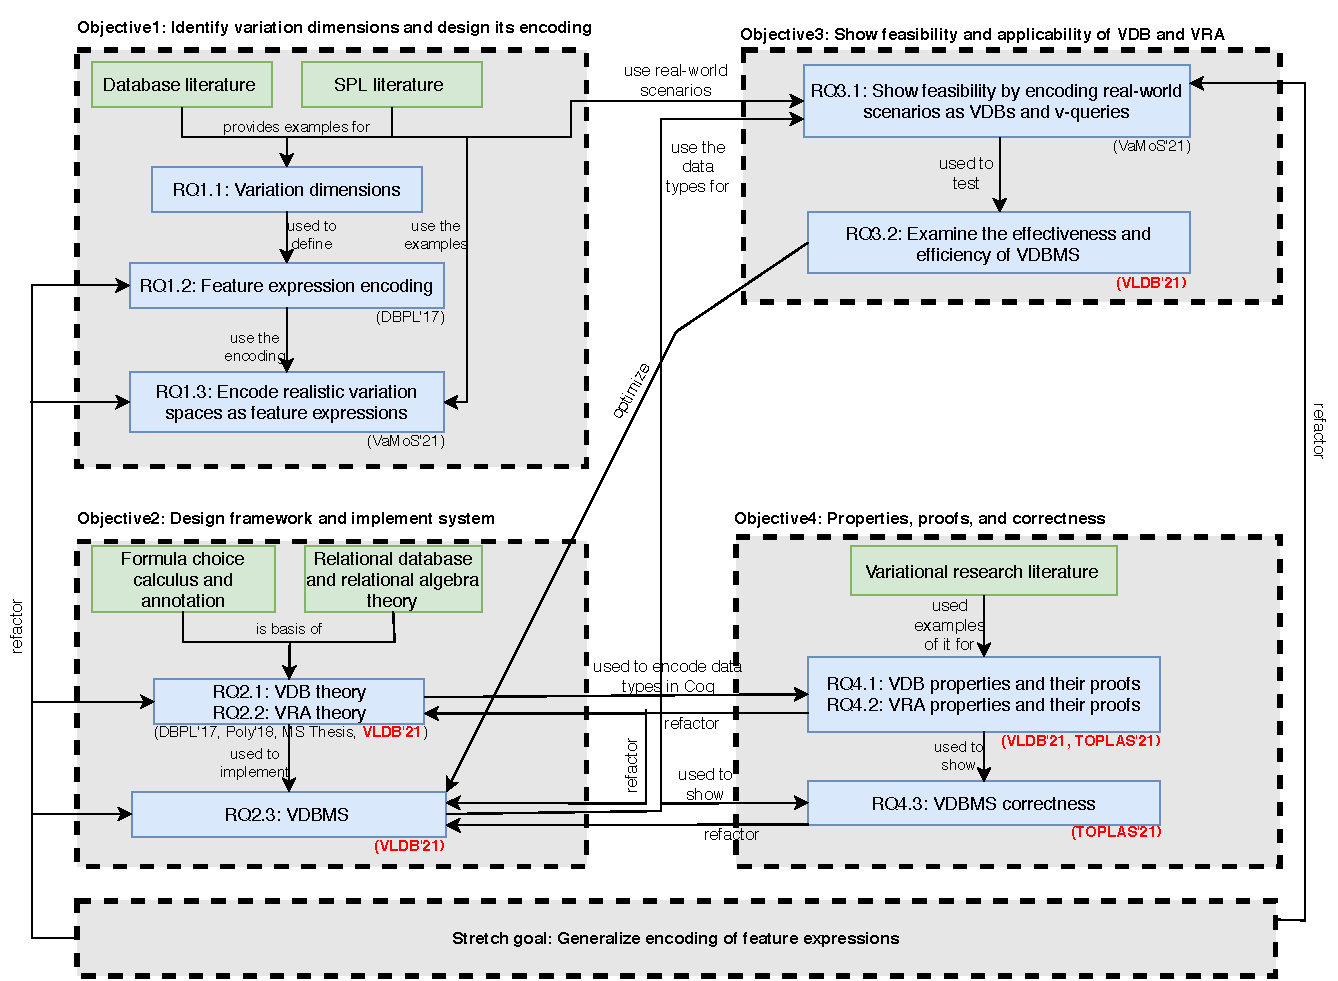
\includegraphics[scale = 0.75] {figs/conn3.pdf}
\caption{The connection between objectives and research questions.
The bolden publications in red are the ones that haven't been submitted yet.}
\label{fig:conn}
\end{figure}

\begin{table}[H]
\label{tab:timeline}
\caption{Summary of projected and completed dates for each of the proposed research questions.}
\centering
\begin{tabular}{|c|c|c|c|}
\hline
Research Question & Target conference & Projected Date & Status\\
\hline
1.1 & \poly & N/A & Complete\\
\hline
1.2 & \dbpl & N/A & Complete\\
\hline
1.3 &  \vamos &N/A & Complete\\
\hline
2.1 & \poly, \dbpl, \vldb &N/A & Complete\\
\hline
2.2 & \poly, \dbpl, \vldb &N/A & Complete\\
\hline
2.3 & \vldb & Early 2021 & In progress\\
\hline
3.1 & \vamos &N/A & Complete\\
\hline
3.2 & \vldb &Early 2021 & In progress\\
\hline
4.1 & \vamos &N/A & Complete\\
\hline
4.2 & \vldb, \toplas & Mid 2021 & In progress\\
\hline
4.3 & \toplas & Mid 2021 & Not started\\
\hline
\end{tabular}
\end{table}


\section{Related Work}
\label{sec:rw}

\subsection{Variational Research}
\label{sec:var-res}

\subsection{Forms of Variation in Relational Databases}
\label{sec:var-in-db}

\textbf{Database Evolution:}

\textbf{Data Integration:}

\textbf{Versioning a Database:}



\section{Conclusion}
\label{sec:con}

Informed by different kinds of variation appearing in databases, we hypothesize that considering 
variation as an orthogonal concern to databases provides benefits to researchers, database administrators, and developers.
To investigate this hypothesis, we planed the following:

\begin{itemize}
\item Activity 1: We have studied various kinds of variation in databases and based on them
we have provided a framework that considers variation as an orthogonal concern of databases~\cite{ATW17dbpl,ATW18poly}.
\item Activity 2: We have used the framework to represent realistic scenarios of variation in databases,
showing the applicability of our framework~\cite{ALW21vamos}.
\item Activity 3: We are implementing and refactoring VDBMS, a database management system for our
framework.
\item Activity 4: We will mechanically prove the properties of our framework.
\end{itemize}

\noindent
The result of these activities will provide the following contributions:

\begin{itemize}
\item The first work to establish a theoretical framework for variational databases that considers variation as an orthogonal concern to databases. (Activity 1 and 4)
\item The first database management system that allows developers and database administrators to interact with variational databases. (Activity 1, 2, and 3)
\item Realistic case studies of variation in databases that can be used in future research on variational data. (Activity 2)
\end{itemize}

The database community has researched different kinds of variation in databases extensively without 
acknowledging that they are instances of the same problem. On the other
hand, the SPL community has realized the need for encoding variation in the data model, however,
they do not go beyond the data model. Our work on RQ1.1 and RQ1.3~\cite{ALW21vamos} has
shown that different instances of variation in databases could interact with each other, thus, 
having a generic encoding of variation in databases is beneficial. 



\newpage
\bibliographystyle{plainnat}
%\bibliographystyle{ACM-Reference-Format}
\bibliography{bib/eric,bib/martin,bib/vdbms,bib/change,bib/vds,bib/fp,bib/error-reporting,bib/misc,bib/dblp2_short,bib/variational,bib/db}

% \newpage
\appendix

\end{document}
